\chapter{Conceitos fundamentais}\label{CAP_CONCEITOS_FUNDAMENTAIS}

%Isto será removido após a revisão
Seguem as críticas da qualificação sobre a seção ``Conceitos fundamentais'':
\begin{enumerate}
\item \textcolor{red}{Explicar como foram organizadas as coleções de workflows.}
\item \textcolor{blue}{Vírgulas.}
\item \textcolor{red}{Definir o termo \emph{itemset} na descrição do algoritmo Apriori.}
\item \textcolor{red}{A frase: ``termos raros são mais informativos que os termos comuns de uma ontologia'' foi criticada. De acordo com o Norton isso pode não ser verdade para sinônimos raros ou termos novos. Acho que uma solução seria achar uma referência para isso.}
\item \textcolor{red}{Colocar o termo ``Apriori'' em itálico.}
\item \textcolor{blue}{A seção métricas de validação ficou confusa, o Norton não entendeu se removiamos atividades do conjunto de teste ou validação.}
\item \textcolor{blue}{Na seção ``Sistemas Gerenciadores de Workflow Científico'' devo adicionar um exemplo completo e explicativo sobre workflow científico.}
\item \textcolor{blue}{A Figura 1(Exemplo do Kepler estava com baixa qualidade) vou colocar várias figuras com alta qualidade.}
\item \textcolor{blue}{A técnica ``community-based'' precisa ter a ordem invertida para ficar mais clara sua relação com o filtro colaborativo.}
\item \textcolor{blue}{Usar todos os termos em apenas um idioma: ``Colaborative filter'' e ``Filtro colaborativo''.}
\item \textcolor{blue}{As equações das várias métricas de distância precisam ter referências.}
\item \textcolor{blue}{Definir o termo ``Shim''.}
\item \textcolor{blue}{Detalhar mais as diversas partes de uma ontologia: i) conceitos; ii) relações; etc.}
\item \textcolor{red}{Achar os autores originais que criaram as técnicas e citar estes.}
\item \textcolor{blue}{Explicar em mais detalhes a ontologia de workflows proposta por bergman e GIL. Eu removi ela, foi usada para composição e não tem nada de bioinformática}
\item \textcolor{blue}{O termo: `` baseada'' trocar por `` partir de''.}
\item \textcolor{blue}{O termo: ``base de dados de workflows científicos'' trocar por `` banco de dados de workflows científicos''.}
\item \textcolor{blue}{Evitar frases grandes.}
\item \textcolor{blue}{Explicar em detalhes o que cada figura representa ao invés de apenas citar.}
\item \textcolor{blue}{A seção métricas de validação deveria revisar os conceitos das métricas ao invés de explicar como serão utilizadas.}
\item \textcolor{blue}{Adicionar figuras explicando a estratégia de testes.}
\end{enumerate}

\newpage
%Isto será removido após a revisão


Este capítulo define os conceitos necessários para compreender a proposta deste mestrado, as cinco primeiras seções definem os conceitos da área de domínio, sistemas de recomendação, ontologias e métricas de validação. Os três últimos capítulos descrevem conceitos relativos a técnicas de recomendação da literatura correlata, classificadores e regressores.

Primeiramente são definidos os sistemas gerenciadores de \emph{workf\mbox{}lows} científ\mbox{}icos e suas características principais (seção \ref{SEC_SISTEMA_GERENCIADOR_WORKFLOW}). As duas seções seguintes (\ref{SEC_SISTEMAS_RECOMENDACAO} e \ref{SEC_RECOMENDACAO_WORKFLOW_CIENTIFICO}) detalham os tipos mais comuns de sistemas de recomendação (genéricos) e desafios para construir um sistema de recomendação de atividades em \emph{workf\mbox{}lows} científ\mbox{}icos. A próxima seção (\ref{SEC_ONTOLOGIA}) define o que é uma ontologia, suas características, formas de uso e definição de termos. A seção imediata (\ref{SEC_METRICAS_VALIDACAO}) descreve quais métricas foram utilizadas para comparar as técnicas propostas com as da literatura correlata. 

A antepenúltima seção (\ref{SEC_RECOMENDACAO_BASE_WORKFLOWS}) define conceitos para recomendar atividades usando banco de dados de \emph{workf\mbox{}lows}. As últimas duas seções (\ref{SEC_RECOMENDACAO_CLASSIFICACAO} e \ref{SEC_RECOMENDACAO_REGRESSAO}) descrevem em detalhes os classificadores e regressores utilizados para recomendar atividades.


\section{Sistemas gerenciadores de \emph{workf\mbox{}lows} científ\mbox{}icos}\label{SEC_SISTEMA_GERENCIADOR_WORKFLOW}
Sistemas gerenciadores de \emph{workflows} científicos (SGWC) são infraestruturas de \emph{software} que permitem a construção, reutilização e captura de proveniência experimentos científicos representados na forma de \emph{workflows} \cite{McPhillips2009}. Os quais possibilitam modelar e executar soluções computacionais para problemas científicos, combinando dados e operações sobre dados em estruturas configuráveis formadas por atividades \cite{Garijo2014}.

As funcionalidades típicas de um SGWC (neste exemplo o Kepler~\cite{kepler2014}) são apresentadas em quatro regiões da Figura~\ref{figura_SGWC_Kepler_exemplo_de_workflow}. A primeira área (\textbf{A}), oferece uma lista de atividades para serem usadas na construção do \emph{workf\mbox{}lows}. A segunda região (\textbf{B}), apresenta os parâmetros de entrada/saída da atividade \textbf{2}. O terceiro espaço (\textbf{C}) permite arrastar atividades e conectá-las, este espaço gráfico é responsável por criar o experimento computacional. A última região (\textbf{D}) apresenta os conectores das atividades (setas pretas e brancas), controle de execução do \emph{workflows} (seta azul e sinal de pause) e as ferramentas de ampliar ou reduzir a área \textbf{C} (lupas).
\begin{figure}[!htb]
    \centering  
    \caption[Sistema gerenciador de \emph{workf\mbox{}low} científ\mbox{}ico Kepler]{Sistema gerenciador de \emph{workf\mbox{}lows} científ\mbox{}icos Kepler.}
    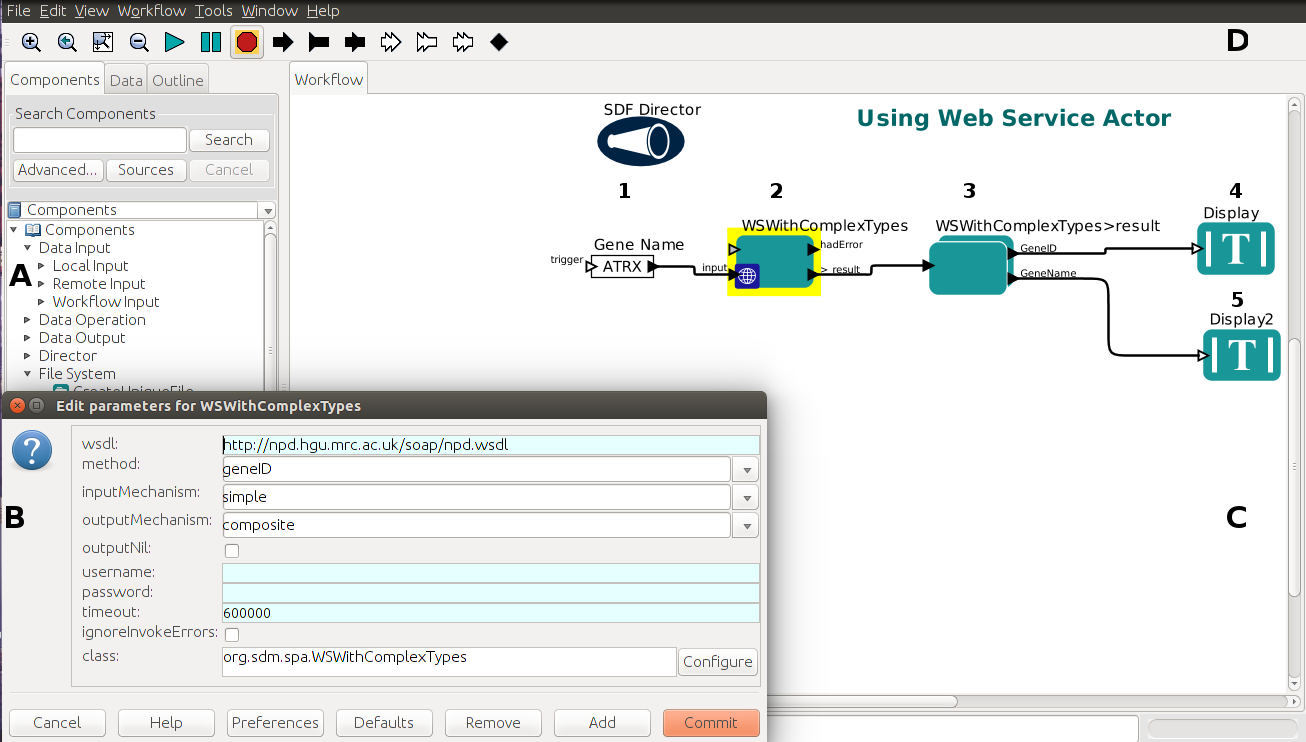
\includegraphics[width=13cm,height=7cm]{./secoes/conceitosFundamentais/pics/img/webService.png}    
	\label{figura_SGWC_Kepler_exemplo_de_workflow}
	\source{Exemplo de \emph{workf\mbox{}low} fornecido pelo sistema Kepler~\cite{kepler2014}.}
\end{figure}

Dentro da área \textbf{C} há um \emph{workf\mbox{}low}, que representa um experimento computacional, o qual recebe o nome de um genee retorna duas informações: i) nome do gene; e ii) identificador na base de dados. Para compreender o processo de construção deste experimento primeiro serão descritas as funcionalidades de cada atividade e em seguida como funciona o fluxo de dados entre estas.

O objetivo das atividades é efetuar algum tipo de processamento nos dados (ou usá-los para pesquisa), como os métodos/funções das linguagens de programação, na Figura \ref{figura_SGWC_Kepler_exemplo_de_workflow} a atividade número \(\mathbf{1}\) recebe o nome do gene que será pesquisado. A número \(\mathbf{2}\) é o cliente do serviço web e recebe como parâmetros: i) o \emph{wsdl} do serviço; ii) o nome do método a ser utilizado; iii) o tipo de retorno do serviço; e iv) as entradas e saídas do método. A número \(\mathbf{3}\) separa as saídas obtidas da pesquisa e envia-as para as atividades \(\mathbf{4}\) e \(\mathbf{5}\) que exibem o resultado na tela.

O fluxo de dados entre atividades pode ocorrer de várias formas, conhecidas por \emph{Model of Computation} (MoC) \cite{Ludascher2006}, workflows científicos em bioinformática usam duas formas de MoC. \emph{Dataflow}, que realiza transformações sobre os dados, analisa/visualiza-os e elabora simulações e \emph{control flow} mais utilizado em \emph{workflows} de negócio, enfatiza eventos, fluxogramas e sequências de atividades. Os workflows de bioinformática usam esses dois MoC de forma híbrida nos experimentos, na Figura \ref{figura_SGWC_Kepler_exemplo_de_workflow} é usado o diretor SDF do Kepler (MoC \emph{dataflow}).

\subsection{Construção de \emph{workf\mbox{}lows} científ\mbox{}icos}
A construção de workflows científicos ocorre pela conexão de diversas atividades, como exibido na Figura \ref{figura_SGWC_Kepler_exemplo_de_workflow}, as quais podem ser rotuladas de acordo com sua estrutura em três classes de atividades. A primeira é conhecida por \emph{atividade simples} que contém apenas uma atividade  \cite{Garijo2012} como na Figura \ref{figura_atividade_simples} com suas entradas (um inteiro e uma \emph{string}) no lado direito, as saídas no lado esquerdo (três inteiros) e internamente o processamento dos dados.
\begin{figure}[!htb]
    \centering  
    \caption{Exemplo de atividade simples.}
    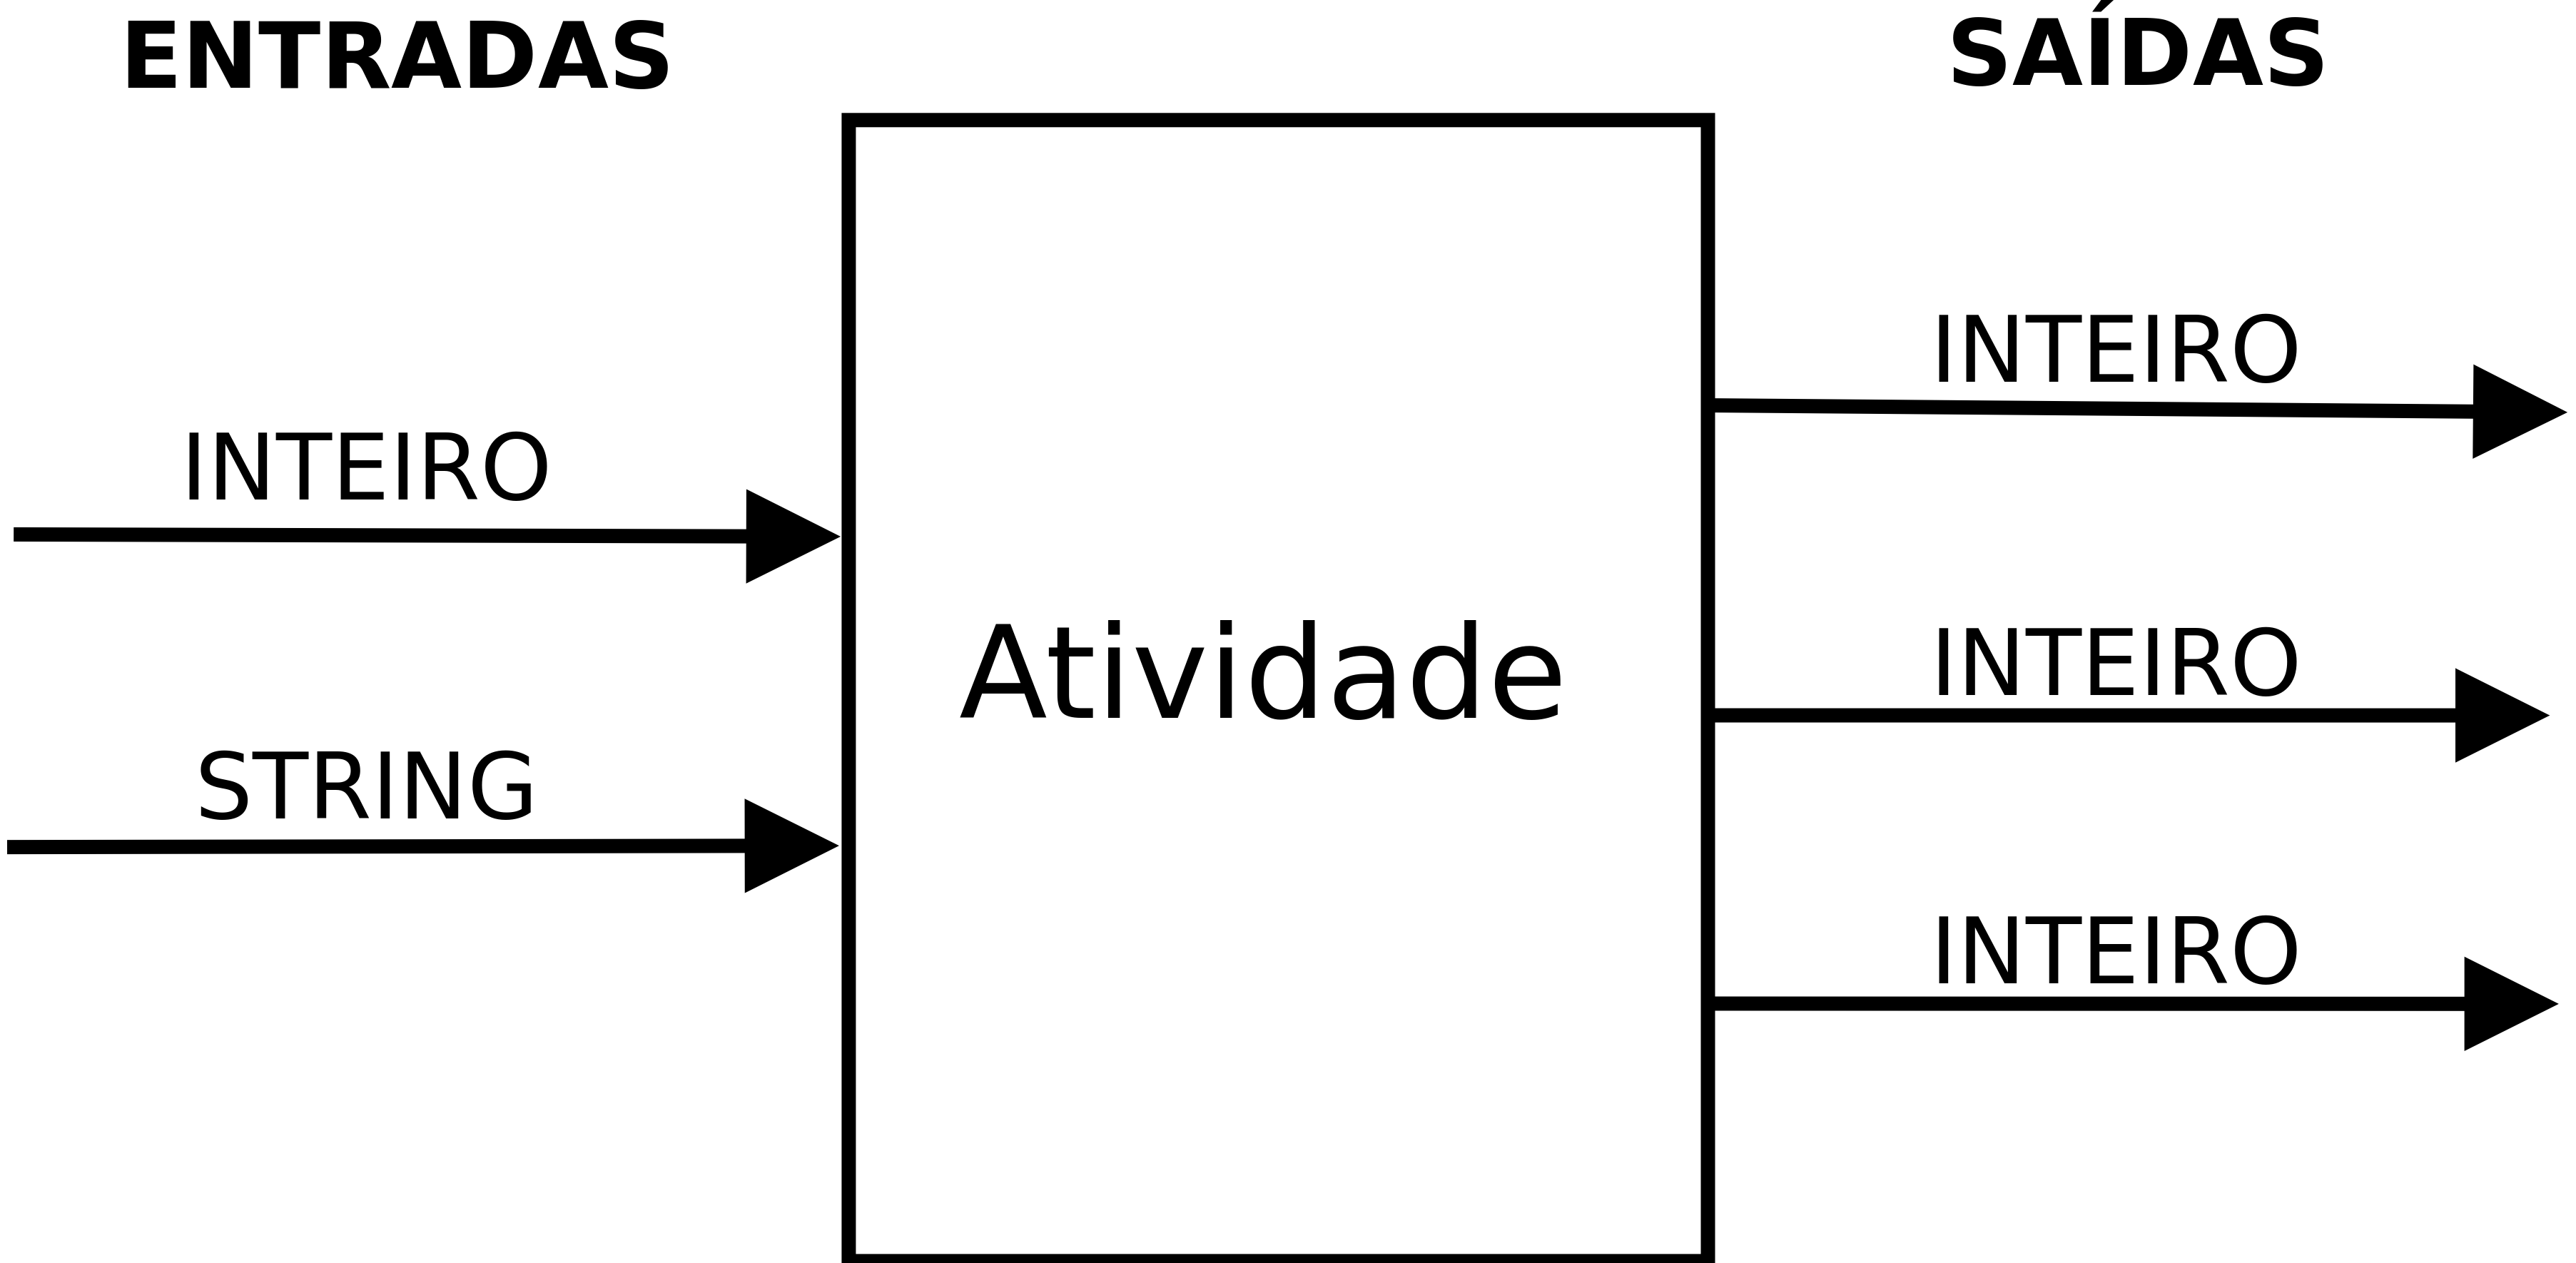
\includegraphics[width=7cm,height=4cm]{./secoes/conceitosFundamentais/pics/img/Atividade.png}    
	\label{figura_atividade_simples}
	\source{\varAutorData.}
\end{figure}

O segundo tipo de atividade é denominado \emph{Shim}, tem por objetivo adapatar diferentes tipos de dados, a qual é exibida na Figura \ref{figura_atividade_shim} \emph{a}. Onde a \emph{atividade} \(1\) tem como saída um \emph{id} do tipo \emph{long} e a atividade \(2\) tem como entrada um \emph{id} do tipo inteiro, como consequência ambas são incompatíveis. As atividades do tipo \emph{Shim} efetuam conversões de tipos de dados permitindo a conexão entre atividades incompatíveis como na \ref{figura_atividade_shim} \emph{b} \cite{Lin2009}.
\begin{figure}[!htb]
    \centering  
    \caption{Exemplo de atividade do tipo \emph{Shim}.}
    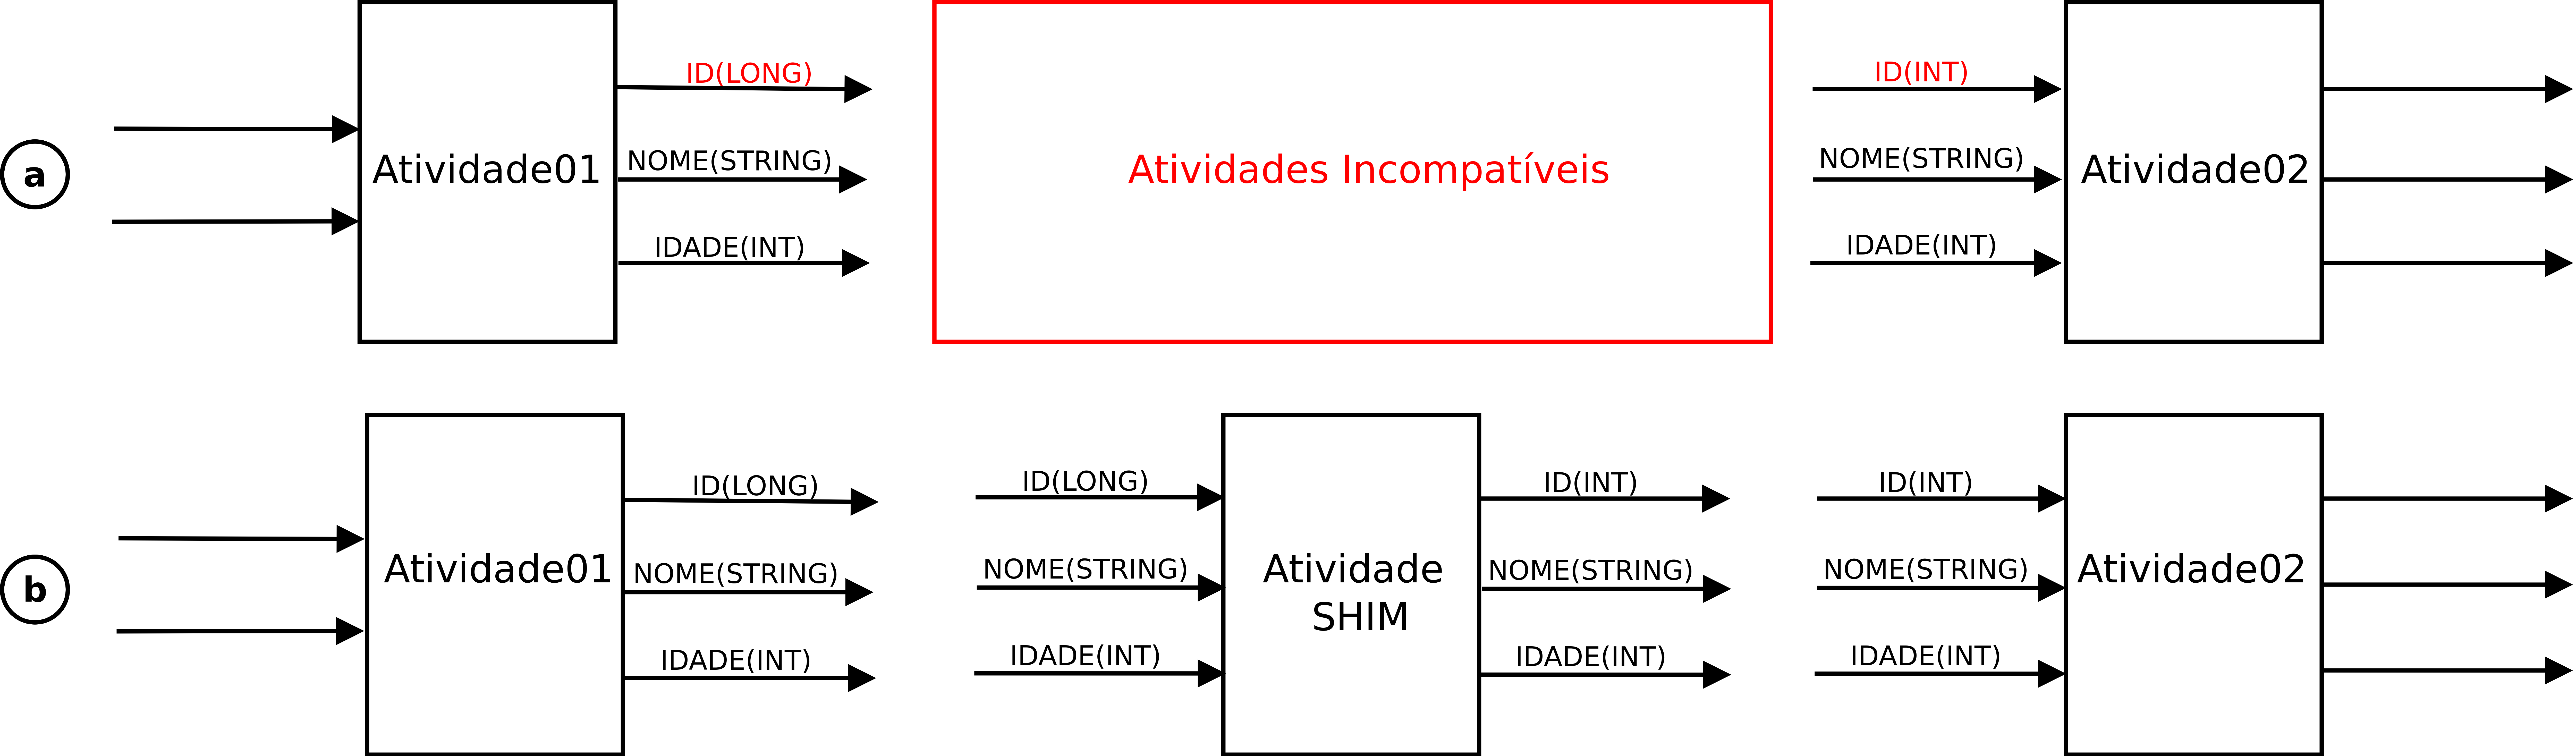
\includegraphics[width=10cm,height=5cm]{./secoes/conceitosFundamentais/pics/img/Shim.png}    
	\label{figura_atividade_shim}
	\source{\varAutorData.}
\end{figure}

O terceiro tipo é denominado \emph{subworkflow}, que é uma atividade constituída por um workflow interno (conjunto de outras atividades), exibido na Figura \ref{figura_atividade_subworkflow} \cite{medeiros_woodss_2005}. Neste caso o processamento da atividade é efetuado por um workflow completo suas entradas e saídas (em verde na figura) devem conter no mínimo as entradas e saídas do workflow interno.
\begin{figure}[!htb]
    \centering  
    \caption{Exemplo de atividade do tipo \emph{subworkflow}.}
    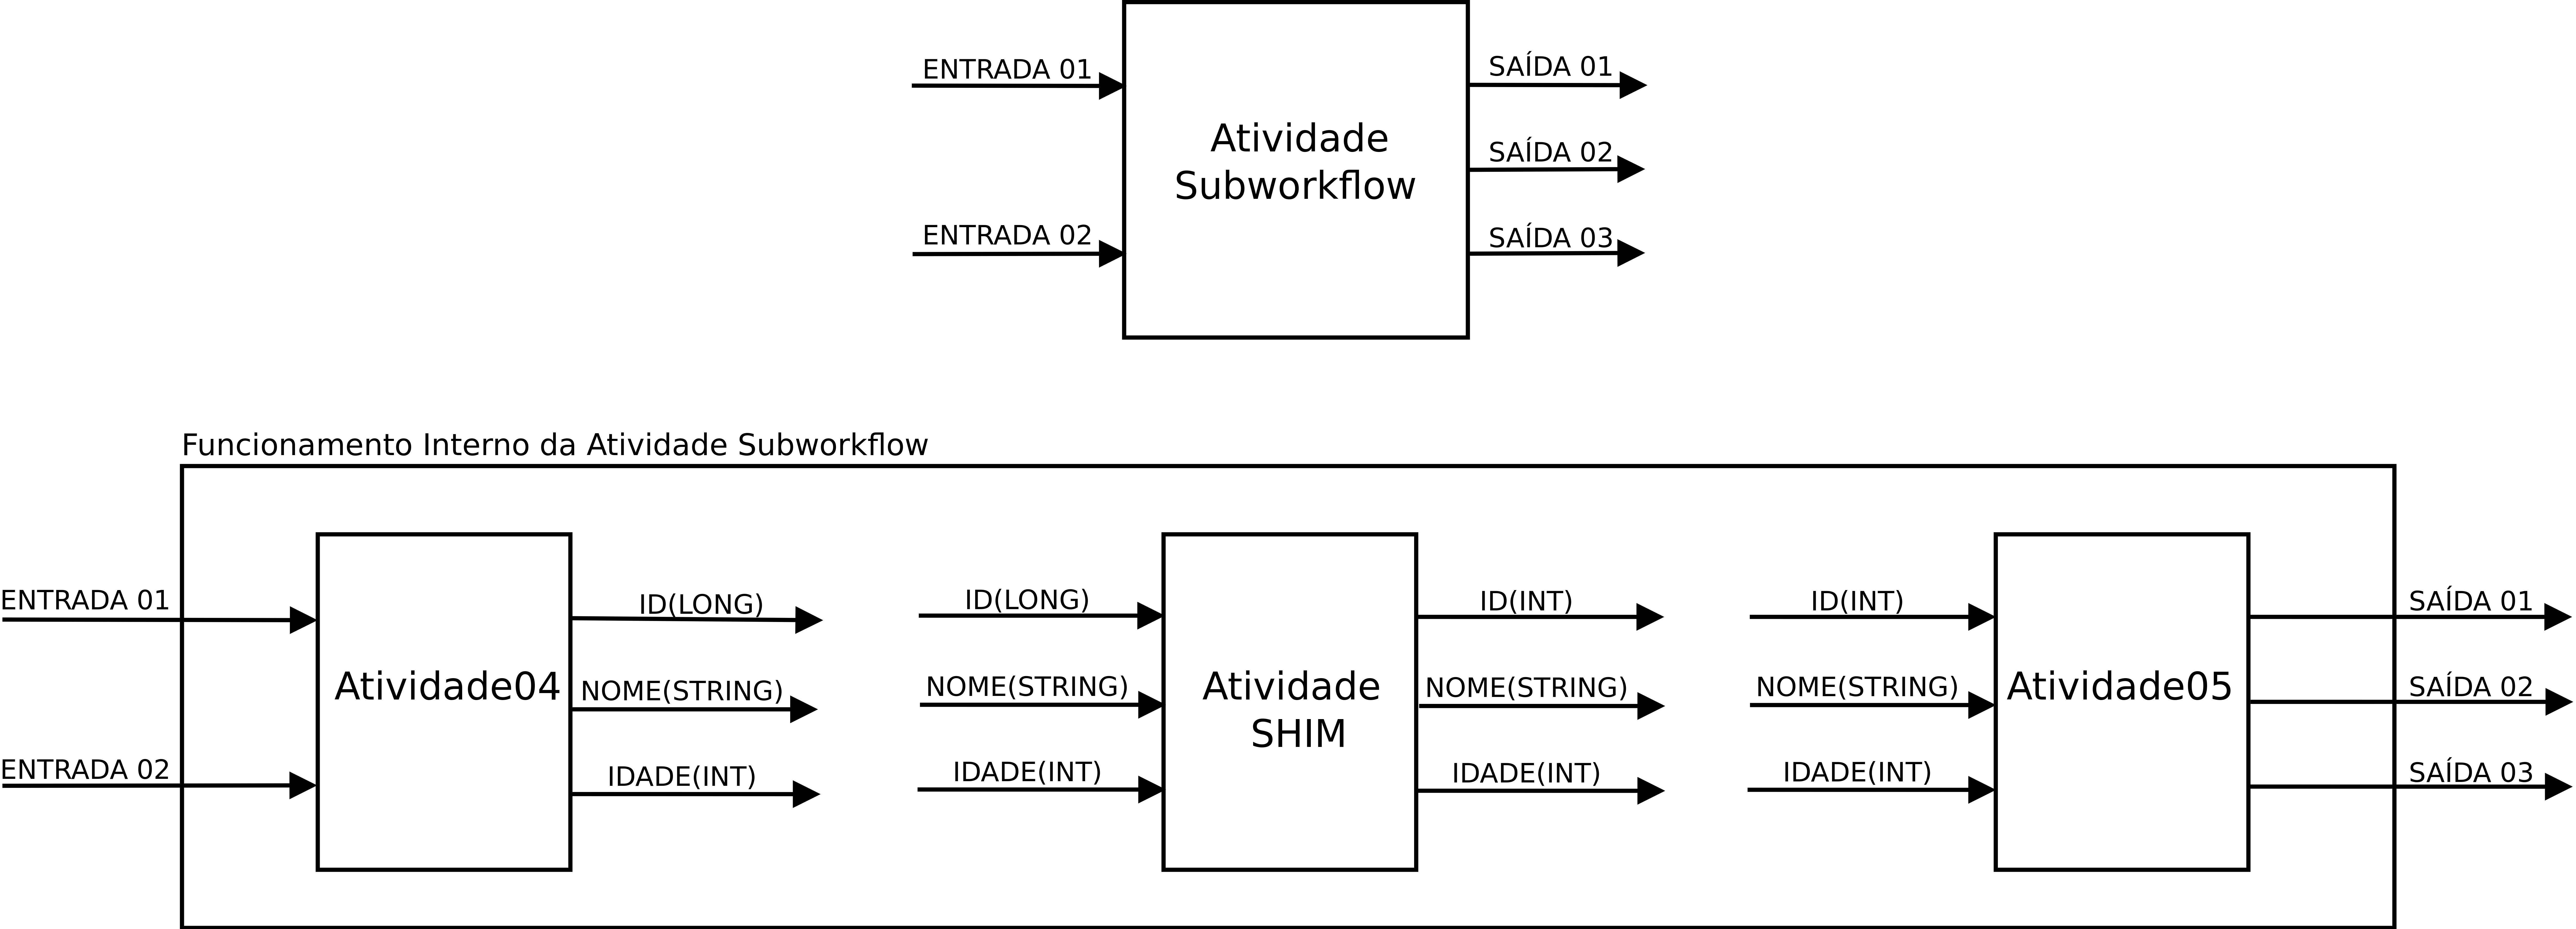
\includegraphics[width=15cm,height=7cm]{./secoes/conceitosFundamentais/pics/img/Subworkflow.png}    
	\label{figura_atividade_subworkflow}
	\source{\varAutorData.}
\end{figure}
Os diferentes tipos de estruturas de atividades faz com que o processamento interno de cada tipo possa ser realizado de diversas formas. A mais comuns é usar um serviço web ou código fonte interno, porém no caso de subworkflows é comum usar um processamento misto. 

Durante a construção do workflow (conexão dos diferentes tipos de atividades) alguns SGWC armazenam as informações relativas a modelagem e execução dos workflows, estas informações são conhecidas como proveniência. Segundo \citeonline{Lim2010} há dois tipos de proveniência: i) \emph{prospective provenance} que modela a especificação de um \emph{workflow}, funcionando como uma abstração/receita do mesmo e pode ser capturada durante a construção; e ii) \emph{retrospective provenance} que modela as execuções dos \emph{workflows}, quais tarefas foram executadas e quais transformações sobre os dados ocorreram, esse tipo de proveniência pode ser capturado durante a execução do \emph{workflow}.

Para auxiliar na construção de workflows foram propostas técnicas para compor automaticamente ou recomendar atividades. A primeira consiste em definir o problema a ser modelado e o sistema gerenciador conecta automaticamente as atividades construindo \emph{workflows} para o usuário, essa técnica é recomendada para usuários que não conhecem detalhes específicos do processo e/ou não desejam se envolver nas especificidades de como o \emph{workflow} irá resolver o problema modelado. A segunda ocorre durante a construção manual das atividades e o sistema gerenciador sugere ao usuário algumas atividades que podem ser úteis para o \emph{workflow} em construção. 

A sugestão de atividades geralmente é baseada em medidas de similaridade (ver seção \ref{SEC_SISTEMAS_RECOMENDACAO}) ou buscando-se atividades em \emph{workflows} parecidos com o que está sendo desenvolvido ou buscando-se atividades usadas por usuários com o mesmo perfil do usuário atual. A técnica de recomendação é indicada para usuários mais experientes que desejam ter participação ativa na construção do \emph{workflow}.


\section{Sistemas de recomendação}\label{SEC_SISTEMAS_RECOMENDACAO}
Sistemas de recomendação têm como objetivo recomendar itens que sejam interessantes aos usuários, formalizando: seja \(C\) o conjunto de todos os usuários, \(S\) o conjunto de todos os itens que podem ser recomendados, \(u\) a função de utilidade que metrifica o quanto um item \(s\) é útil para um determinado usuário \(c\), \(u:C \times S\rightarrow R\) onde \(R\) é um conjunto totalmente ordenado. Para cada usuário \(c \in C \) queremos escolher \(s^{'} \in S \) que maximize a função de utilidade 
\begin{align}
\forall c \in C,  \quad s_{c}^{'} =  \operatorname*{arg\,max}_{s \in S} u(c,s) \label{formalizar_recomendacao}
\end{align}

Em sistemas de recomendação a função utilidade \(u\) não está definida para todo o espaço \(C \times S\), isso força os sistemas de recomendação a extrapolar o espaço conhecido \cite{Adomavicius2005}.

Para solucionar esse problema foram propostas diferentes técnicas para recomendar itens, as quais \citeonline{Paiva2013} classificam em seis grupos. A primeira, chamada \emph{filtro baseado em conteúdo}, recomenda itens similares a outros selecionados anteriormente pelo próprio usuário, suas limitações são: i) análise limitada do conteúdo do item que será recomendado, geralmente há falta de descrição semântica do item; ii) superespecialização quando o usuário recebe recomendações similares demais as suas escolhas; e iii) novos usuários precisam avaliar um número mínimo de itens antes que o sistema possa recomendar itens para ele.

A segunda, denominada \emph{filtro colaborativo}, recomenda itens que já foram selecionados por outros usuários \emph{similares}, tem como limitações: i) o problema de novos usuários (como identificar com quem eles são similares?); ii) novos itens somente serão recomendados ao passo que forem sendo avaliados por usuários; iii) dados esparsos, alguns poucos usuários costumam avaliar muitos itens e a maioria avalia poucos itens tornando a matriz de utilidade (usuários \(\times\) itens) esparsa, pois o número de avaliações feitas tende a ser muito menor do que o número de sugestões a serem realizadas. Dessa forma, itens raros (que foram avaliados por poucos) dificilmente serão recomendados.

A terceira, são as estratégias híbridas, combina características das técnicas existentes tentando minimizar suas limitações.

A quarta, conhecida por \emph{filtro baseado na comunidade}, a recomendação é realizada de acordo com a preferência dos colegas e amigos do usuário ao invés de preferências de desconhecidos, é um tipo de especialização do filtro colaborativo herdando suas características. Em outras palavras, é baseada em informações da rede social (comunidade) do usuário.

A quinta, chamada \emph{demográfica}, utiliza atributos como região, idade, idioma para recomendar, surgiu para tentar minimizar o problema de esparsidade e é uma especialização do filtro colaborativo considerando que usuários com mesmos dados demográficos podem ser considerados similares.

A sexta, \emph{baseado em conhecimento}, recomenda itens de acordo com o domínio de aplicação, a função de similaridade estima quanto a descrição do problema é similar a solução recomendada. Tem como limitação a necessidade de descrições semânticas (usando, por exemplo, ontologias) sobre o domínio, usuário e o problema.

As técnicas de recomendação citadas necessitam de uma métrica de similaridade para determinar o quanto dois itens/usuários/conceitos são próximos. \citeonline{ZhongLi2009} definem uma função de similaridade genérica \(s\) onde o valor \(s(x,x^{'})\) é alto quando \(x\) e \(x^{'}\) são exemplos parecidos/similares/próximos, caso contrário, possuem um valor baixo. Essa função é simétrica logo \(s(x,x^{'}) = s(x^{'},x), \forall x,x^{'} \in X\) e de uma forma geral tem seu valor normalizado \(0 \leq s(x,x^{'}) \leq 1 \quad \forall x,x^{'} \in X\).

De acordo com \citeonline{ZhongLi2009} distâncias são conhecidas por dissimilaridades, um caso invertido de similaridade onde \(s(x,x^{'})\) é baixo quando \(x\) e \(x^{'}\) são exemplos parecidos ou similares, caso contrário, possuem um valor alto. Uma métrica de similaridade muito utilizada é a distância Euclidiana \cite{Deza2009} calculada por
\begin{align}
d(x,y) = \sqrt{  \sum\limits_{i=1}^{n} |x_{i} - y_{i}|^{2} } \label{dist_euclidiana}
\end{align}
ou a distância de Manhatan \cite{Deza2009} calculada por
\begin{align}
d(x, y) = \sum\limits_{i=1}^{N} |x_{i} - y_{i}|\label{dist_manhattan}
\end{align}
uma similaridade muito conhecida é a da correlação de Pearson \cite{Deza2009} calculada por
\begin{align}
sim(x,y) &= \frac{\sum\limits_{i=1}^{n} (x_{i}-\bar{x})(y_{i} - \bar{y})}
{\sqrt{ \left( \sum\limits_{j=1}^{n}(x_{j}-\bar{x}) \right) ^{2} \left( \sum\limits_{j=1}^{n}(y_{j}-\bar{y})\right)^{2}} } \label{similaridade_pearson}
\end{align}
A distância de Levenshtein \cite{Deza2009} dada por
\begin{align}
d_{L}(x,y) = min\{d_{H}(x^{*}, y^{*})\} \label{dist_Levenshtein}
\end{align}
onde \(x^{*}, y^{*}\) são strings de tamanho \(k, k \leq max(m, n)\). Esta distância representa o número mínimo de alterações para tornar duas \emph{strings} iguais.

\section{Recomendação em \emph{workflows} científicos}\label{SEC_RECOMENDACAO_WORKFLOW_CIENTIFICO}
Construir um sistema de recomendação para \emph{workflows} científicos envolve duas principais tarefas. A primeira é recomendar itens que satisfaçam o usuário (como descrito na equação \eqref{formalizar_recomendacao}). A segunda é resolver problemas específicos da recomendação atividades para \emph{workflows} científicos que são: i) restrições de dependência entre entrada e saída de atividades; ii) dependência semântica entre atividades; e iii) ordem das atividades.

A dependência entre entrada e saída de atividades implica que o tipo de dado (inteiro, \emph{string}, \emph{boolean}) das saídas da atividade anterior devem ser compatíveis com os tipos de dados das entradas da atividade a ser recomendada. Suponha que a atividade \emph{A} tem como saída dois inteiros e uma \emph{string}, dessa forma qualquer outra atividade \emph{B}, a ser recomendada para completar o \emph{workflow} que contém \emph{A} deve ter como entrada dados compatíveis com estes três tipos (ou com um subconjunto deles) ou será necessária a utilização de uma atividade do tipo \emph{Shim}.

Conectar duas atividades por meio de compatibilidade de entrada e saída ou indiretamente, com uso de atividades \emph{Shim} (como na Figura \ref{figura_atividade_shim}) não garante que o \emph{workflow} execute ou que o problema do usuário seja solucionado. Isto ocorre em função da possível incompatibilidade semântica entre atividades como na Figura \ref{figura_Incompatibilidade_Semantica}, 
onde as duas atividades são compatíveis sintáticamente, as entradas e saídas das atividades tem os mesmos tipos de dados, porém a string da atividade \(1\) é o caminho de um arquivo enquanto que a string da atividade \(2\) é uma conexão com base de dados.
\begin{figure}[!htb]
    \centering  
    \caption{Exemplo de incompatibilidade semântica entre atividades.}
    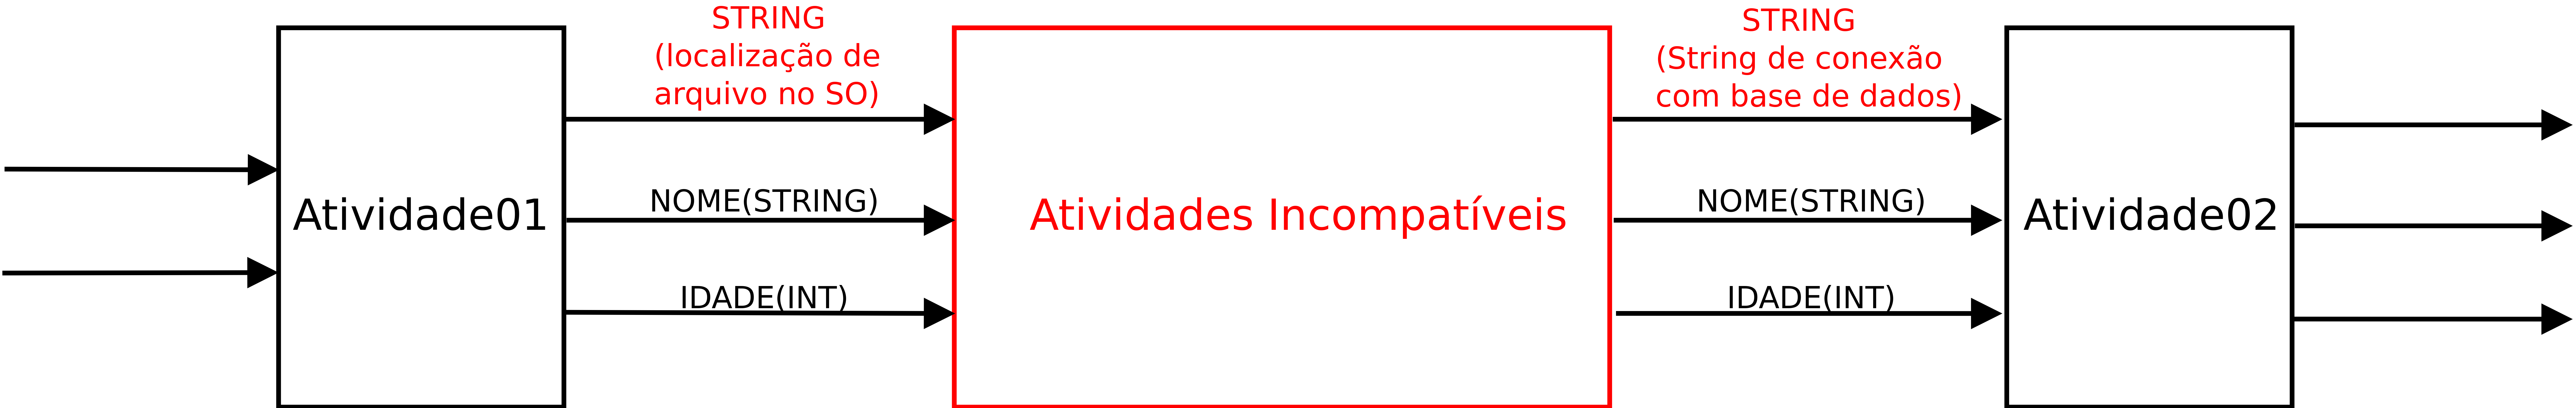
\includegraphics[width=13cm,height=4cm]{./secoes/conceitosFundamentais/pics/img/IncompatibilidadeSemantica.png}    
	\label{figura_Incompatibilidade_Semantica}
	\source{\varAutorData.}
\end{figure}

Além das dependências é necessário conectar as atividades na ordem correta ao contrário de sistemas de recomendação de filmes, onde  pode-se recomendar itens em qualquer ordem sem afetar o resultado final da recomendação, nessa área a ordem das atividades é relevante. Por exemplo, dadas duas atividades: uma que consulte um banco de dados e outra que atualize a informação consultada pela primeira à ordem de execução destas atividades trará diferentes resultados.

Essas características motivaram a criação de técnicas específicas para recomendar atividades em \emph{workflows} científicos, como as citadas no capítulo (\ref{CAP_CORRELATOS}).

%, as quais consideram  validação sintática (entrada e saída de atividades), frequência de uso de atividades, comparação de subgrafos, proveniência de dados, uso de semântica e \emph{itemsets} frequentes.

\section{Ontologias}\label{SEC_ONTOLOGIA}
Ontologia é um modelo de representação de conhecimento utilizado para descrever conceitos de um domínio e suas relações, provendo um vocabulário compartilhado para estes. Os conceitos são os substantivos de um determinado domínio de conhecimento e as relações representam as possíveis interações/hierarquias entre esses conceitos~\cite{Umamaheswari2012}.

Os elementos básicos, mas não obrigatórios, de uma ontologia são quatro. O Primeiro são os conceitos, que são organizados em uma taxonomia e representam a conceitualização de um domínio, e são representados pelos retângulos na Figura \ref{figura_ontologia}. Segundo são as relações, representadas pelas setas da Figura \ref{figura_ontologia}, são as interações entre os conceitos de um determinado domínio. Terceiro são os axiomas que são usados para modelar sentenças. E o último são as instâncias, que representam os elementos específicos, em outras palavras os próprios dados \cite{ALMEIDA2003}. 
\begin{figure}[!htb]
    \centering   
    \caption{Exemplo de ontologia.}
    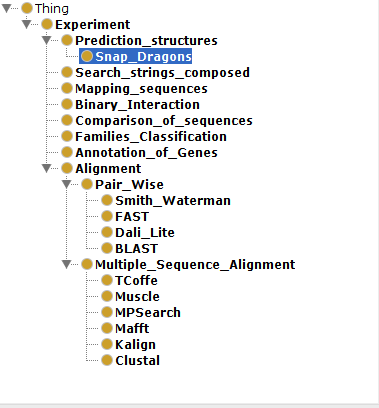
\includegraphics[width=7cm, height=5cm]{./secoes/conceitosFundamentais/pics/img/Ontologia.png}
    \source{Adaptado de \citeonline{Umamaheswari2012}.}
	\label{figura_ontologia}
\end{figure}

Há várias propostas na literatura sobre como classificar ontologias \citeonline{ALMEIDA2003} sumarizam estas propostas na Tabela \ref{tabela_classificacao_ontologias}. Foram encontradas cinco critérios para classificação de ontologia o primeiro é baseado na função desta. A segunda é em relação ao grau de formalismo da linguagem usada, a terceira é em relação a sua aplicação, a quarta é em relação a estrutura (mais genérica ou específica) e a última é em relação ao conteúdo da ontologia.
\bgroup
\def\arraystretch{2}
\begin{table}[htbp]
\tiny
\centering
\caption{Possíveis classificações de ontologias de acordo com a literatura correlata.}
\begin{tabular}{lll}  \hline
\multicolumn{1}{c}{\textbf{Abordagem}} & \multicolumn{1}{c}{\textbf{Classificação}} &  \multicolumn{1}{c}{\textbf{Descrição}} \\  \hline
%Linha 1
\multirow{3}{*}{\parbox{3cm}{Classificação por \emph{Função} proposta por \citeonline{Mizoguchi1995}}} 			& Domínio       		& Fornecem vocabulário sobre conceitos e seus relacionamentos. \\
				                   						& Tarefa        		& Provê vocabulário sistematizado para diferentes domínios.\\
				                   						& Gerais         		& Vocabulário relacionado a eventos, espaço, casualidade.  \\
\hline 
%Linha 2
\multirow{4}{*}{\parbox{3cm}{Classificação por \emph{Grau de formalismo} proposta por  \citeonline{Uschold96ontologies}}} 	& Informal       		& Linguagem natural  \\ [0.1cm] 
										                & Seminformal        	& Linguagem natural restrita.     			 \\ 
										                & Semiformal         	& Linguagem artificial definida formalmente. \\ 
										                & Formal             	& Semântica formal, teoremas e provas.       \\ 
						                
\hline
%Linha 3
\multirow{3}{*}{\parbox{3cm}{Classificação por \emph{Aplicação} proposta por \citeonline{Jasper99aframework}}} 	& Autoria neutra        & Aplicativo escrito para um sistema e usado em outros.         \\ [0.1cm]
									                    & Especificação        	& Criada para a manutenção e desenvolvimento de sistemas.   \\  
									                    & Acesso comum          & Torna o vocabulário inteligível quando este é ininteligível.\\
\hline
%Linha 4
\multirow{3}{*}{\parbox{2.5cm}{Classificação por \emph{Estrutura} proposta por  \citeonline{haav2001context}}} & Alto nível       & Descrevem conceitos gerais não relacionados ao domínio.         \\ 
	                   						& Domínio          		& Descrevem conceitos gerais relacionados ao domínio. \\ 
	                   						& Tarefa           		& Descrevem atividades com escopo inferior aos conceitos de domínio.  \\ 
\hline  
%Linha 5
\multirow{7}{*}{\parbox{3cm}{Classificação por \emph{Conteúdo} proposta por  \citeonline{vanHeijst1997}}} 			& Terminológica     	    & especificam termos usados para representar um domínio.        \\ 
									                    & Informação   		        & Estruturas de registros de bases de dados.         \\ 
									                    & \parbox{2.5cm}{Modelagem de conhecimento} & Especificam conceitualização do conhecimento.         \\
									                    & Aplicação             	& Definições para modelar o conhecimento uma aplicação   \\
									                    & Domínio             		& Conceitualizações específicas de um domínio.  \\ 
									                    & Genérica             		& Conceitualizações genéricas usadas em vários domínios.  \\
									                    & Representação             & Conceitualismo usados para representação do conhecimento.         \\    \hline
\end{tabular}

\label{tabela_classificacao_ontologias}
\source{Adaptado de \citeonline{ALMEIDA2003}.}
\end{table}
\egroup

Para utilizar ontologias em sistemas de recomendação é necessário definir uma métrica de similaridade entre ontologias ou entre conceitos de uma mesma ontologia, a qual, segundo \citeonline{Sanchez2012}, pode ser calculada por três principais abordagens i) contagem por arestas; ii) características da ontologia; e iii) conteúdo da informação. A contagem de arestas utiliza a representação em grafos de ontologias onde cada conceito é representado por um nó e as relações entre os conceitos (por exemplo, relações taxonômicas) são representadas por arestas, essa abordagem calcula o caminho mínimo de arestas entre dois conceitos. Suas principais limitações são não considerar outros possíveis caminhos ou medidas de similaridade (entre conceitos) e utilizar o mesmo peso para todas as arestas.

A abordagem baseada em características das ontologias, utiliza a diferença entre as propriedades em comum dos conceitos e as propriedades diferentes para calcular a similaridade. As propriedades citadas são, por exemplo, os sinônimos ou definições textuais que os conceitos contenham (nas não é mandatório que os conceitos das ontologias contenham essas propriedades). As limitações desta abordagem são exigir que a ontologia tenha propriedades além da taxonomia e a dificuldade de se identificar os pesos corretos a serem atribuídos para cada propriedade \cite{Sanchez2012}.

A abordagem baseada em conteúdo da informação presente nas ontologias calcula a similaridade baseada na coocorrência de termos entre duas ontologias. Por exemplo, utilizando a equação \(IC(x) = -\log_2 P(x)\) que calcula o \(\log_2\) negativo da probabilidade de ocorrência de \(x\), dessa forma, termos raros são considerados mais informativos que os comuns. Sua limitação é que necessita de uma grande e refinada estrutura ontológica/taxonômica para conseguir discriminar diferentes conceitos \citeonline{Sanchez2012}.

\section{Estratégia de validação dos sistemas de recomendação} \label{SEC_METRICAS_VALIDACAO}
Será usado um \emph{\(10\)-fold cross validation}, descrito na Figura \ref{figura_10_fold_cross_validation}, onde
cada fold  usa \(10\%\) dos workflows para testes e \(90\%\) destes treinamento. O qual consiste em apresentar o conjunto de dados rotulados (fica explícito qual atividade foi removida) para os diversos sistemas de recomendação que devem aprender a recomendar com estes exemplos. O teste apresenta os \(10\%\) de workflows, sem informar os rótulos (a atividade removida), para os sistemas de recomendação que já foram treinados. Ao término das dez execuções são calculadas as médias das métricas: i) \emph{Sucess at rank k}(\(S@k\)); ii) \emph{Reciprocal Rank} (RR); e iii) \emph{Reciprocal Rank} (RR).
\begin{figure}[!htb]
    \centering   
    \caption{Exemplo de validação cruzada em dez \emph{folds}.}
    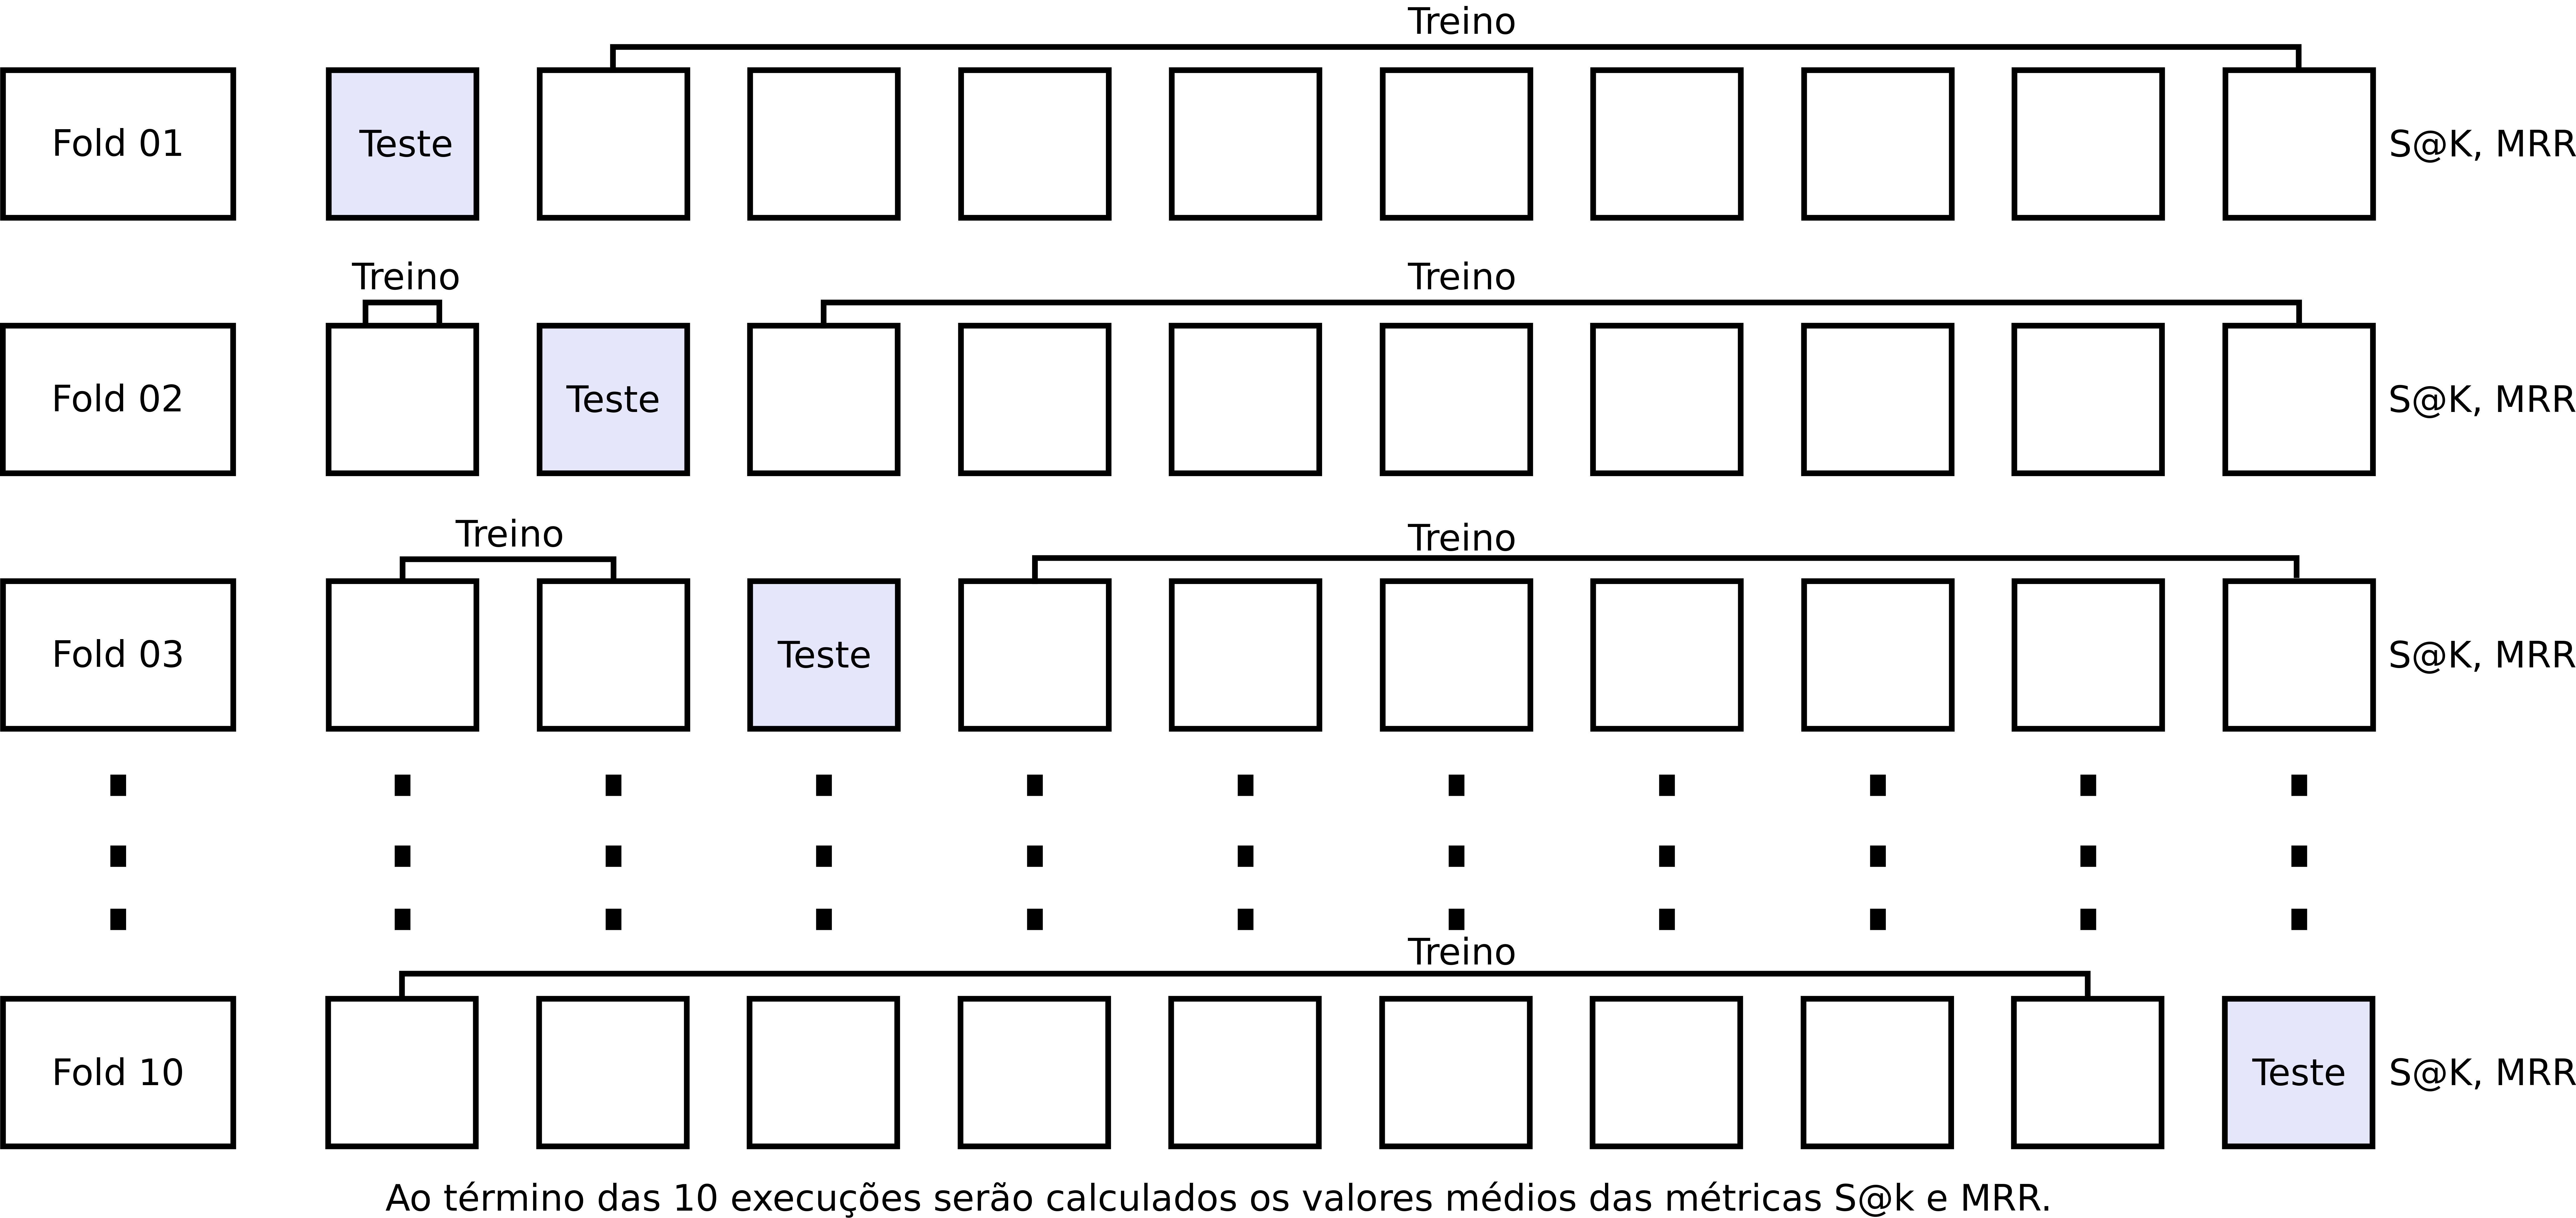
\includegraphics[width=14cm, height=9cm]{./secoes/conceitosFundamentais/pics/img/10FOLDCROSS.png}
    \source{Adaptado de \citeonline{HanKamber2011}.}
	\label{figura_10_fold_cross_validation}
\end{figure}

A métrica \(S@k\) cálcula a probabilidade de um item estar localizado entre as \(k\) primeiras posições da lista de atividades recomendadas, seus valores residem entre zero e um. Os resultados dessa métrica são cumulativos para valores crescentes de \(k\), o que ocorre pois uma atividade que está entre as cinco primeiras posições da lista e consequentemente encontra-se entre as dez primeiras posições. No limite a atividade sempre estará entre as \(L\) primeiras posições, onde \(L\) é o tamanho total da lista de recomendações. Logo é considerado um bom resultado, grandes valores de probabilidade para o menor valor possível de \(k\), ou seja \(S@1 = 1\) é o melhor resultado possível indicando que todas as atividades se encontram na primeira posição das listas recomendadas.

A métrica \(RR\) é o inverso da posição onde o item relevante se encontra na lista de recomendações, seus possíveis valores residem entre zero e um. Quanto maior o valor dessa métrica melhor é o resultado pois uma atividade na primeira posição indica um sistema de recomendação eficiente. Ao retirar a média do \emph{RR} para todas as recomendações obtemos o índice \(MRR\) cujo funcionamento é análogo ao do \emph{RR}

O cálculo dessas métricas é detalhado por \citeonline{Harvey2010} com as equações \eqref{equ_rr}, \eqref{equ_mrr} e \eqref{equ_s@k} dadas por
\begin{align}
RR & = \frac{1}{n_{i}}													\label{equ_rr}\\
MRR &= \frac{1}{N} \sum\limits_{i=1}^{N} \left( \frac{1}{n_{i}} \right) \label{equ_mrr}\\
S@k &= \frac{1}{N} \sum\limits_{i=1}^{N} I(n_{i} \leq k) 				\label{equ_s@k}
\end{align}
onde \(N\) é o número de listas recomendadas, \(n_{i}\) é a posição do item desejado na lista de recomendações \(i\), \(k\) é uma posição da lista determinada como parâmetro de entrada da equação \eqref{equ_s@k} e a função \emph{I}, indica se a atividade \(n_{i}\) ocorre em uma posição menor que o parâmetro de entrada \(k\), e é dada por
\begin{align}
I   &= \begin{cases} \label{equ_indicativa}
			1 \textrm{ se } y_{i} \leq k \\
			0 \textrm{ cc }
	    \end{cases}
\end{align}

Para exemplificar o uso destas métricas será utilizado um workflow fictício representado na Figura \ref{figura_atividades_removidas} que teve quatro atividades removidas (\textbf{B}, \textbf{C}, \textbf{A} e \textbf{Z}) uma a uma gerando quatro casos que necessitam e recomendações (\(\mathbf{1}, \mathbf{2}, \mathbf{3}\) e \(\mathbf{4}\)). Os quais foram usados como entradas para quatro sistemas de recomendação distintos. Cada sistema produziu quatro listas de recomendação, uma para cada caso da Figura \ref{figura_atividades_removidas}, rotulados com a mesma númeração, logo a Lista\(01\) é a recomendação correspondente do caso \(1\) e assim sucessivamente.
\begin{figure}[!htb]
    \centering   
    \caption{Geração de quatro casos de recomendação de atividades.}
    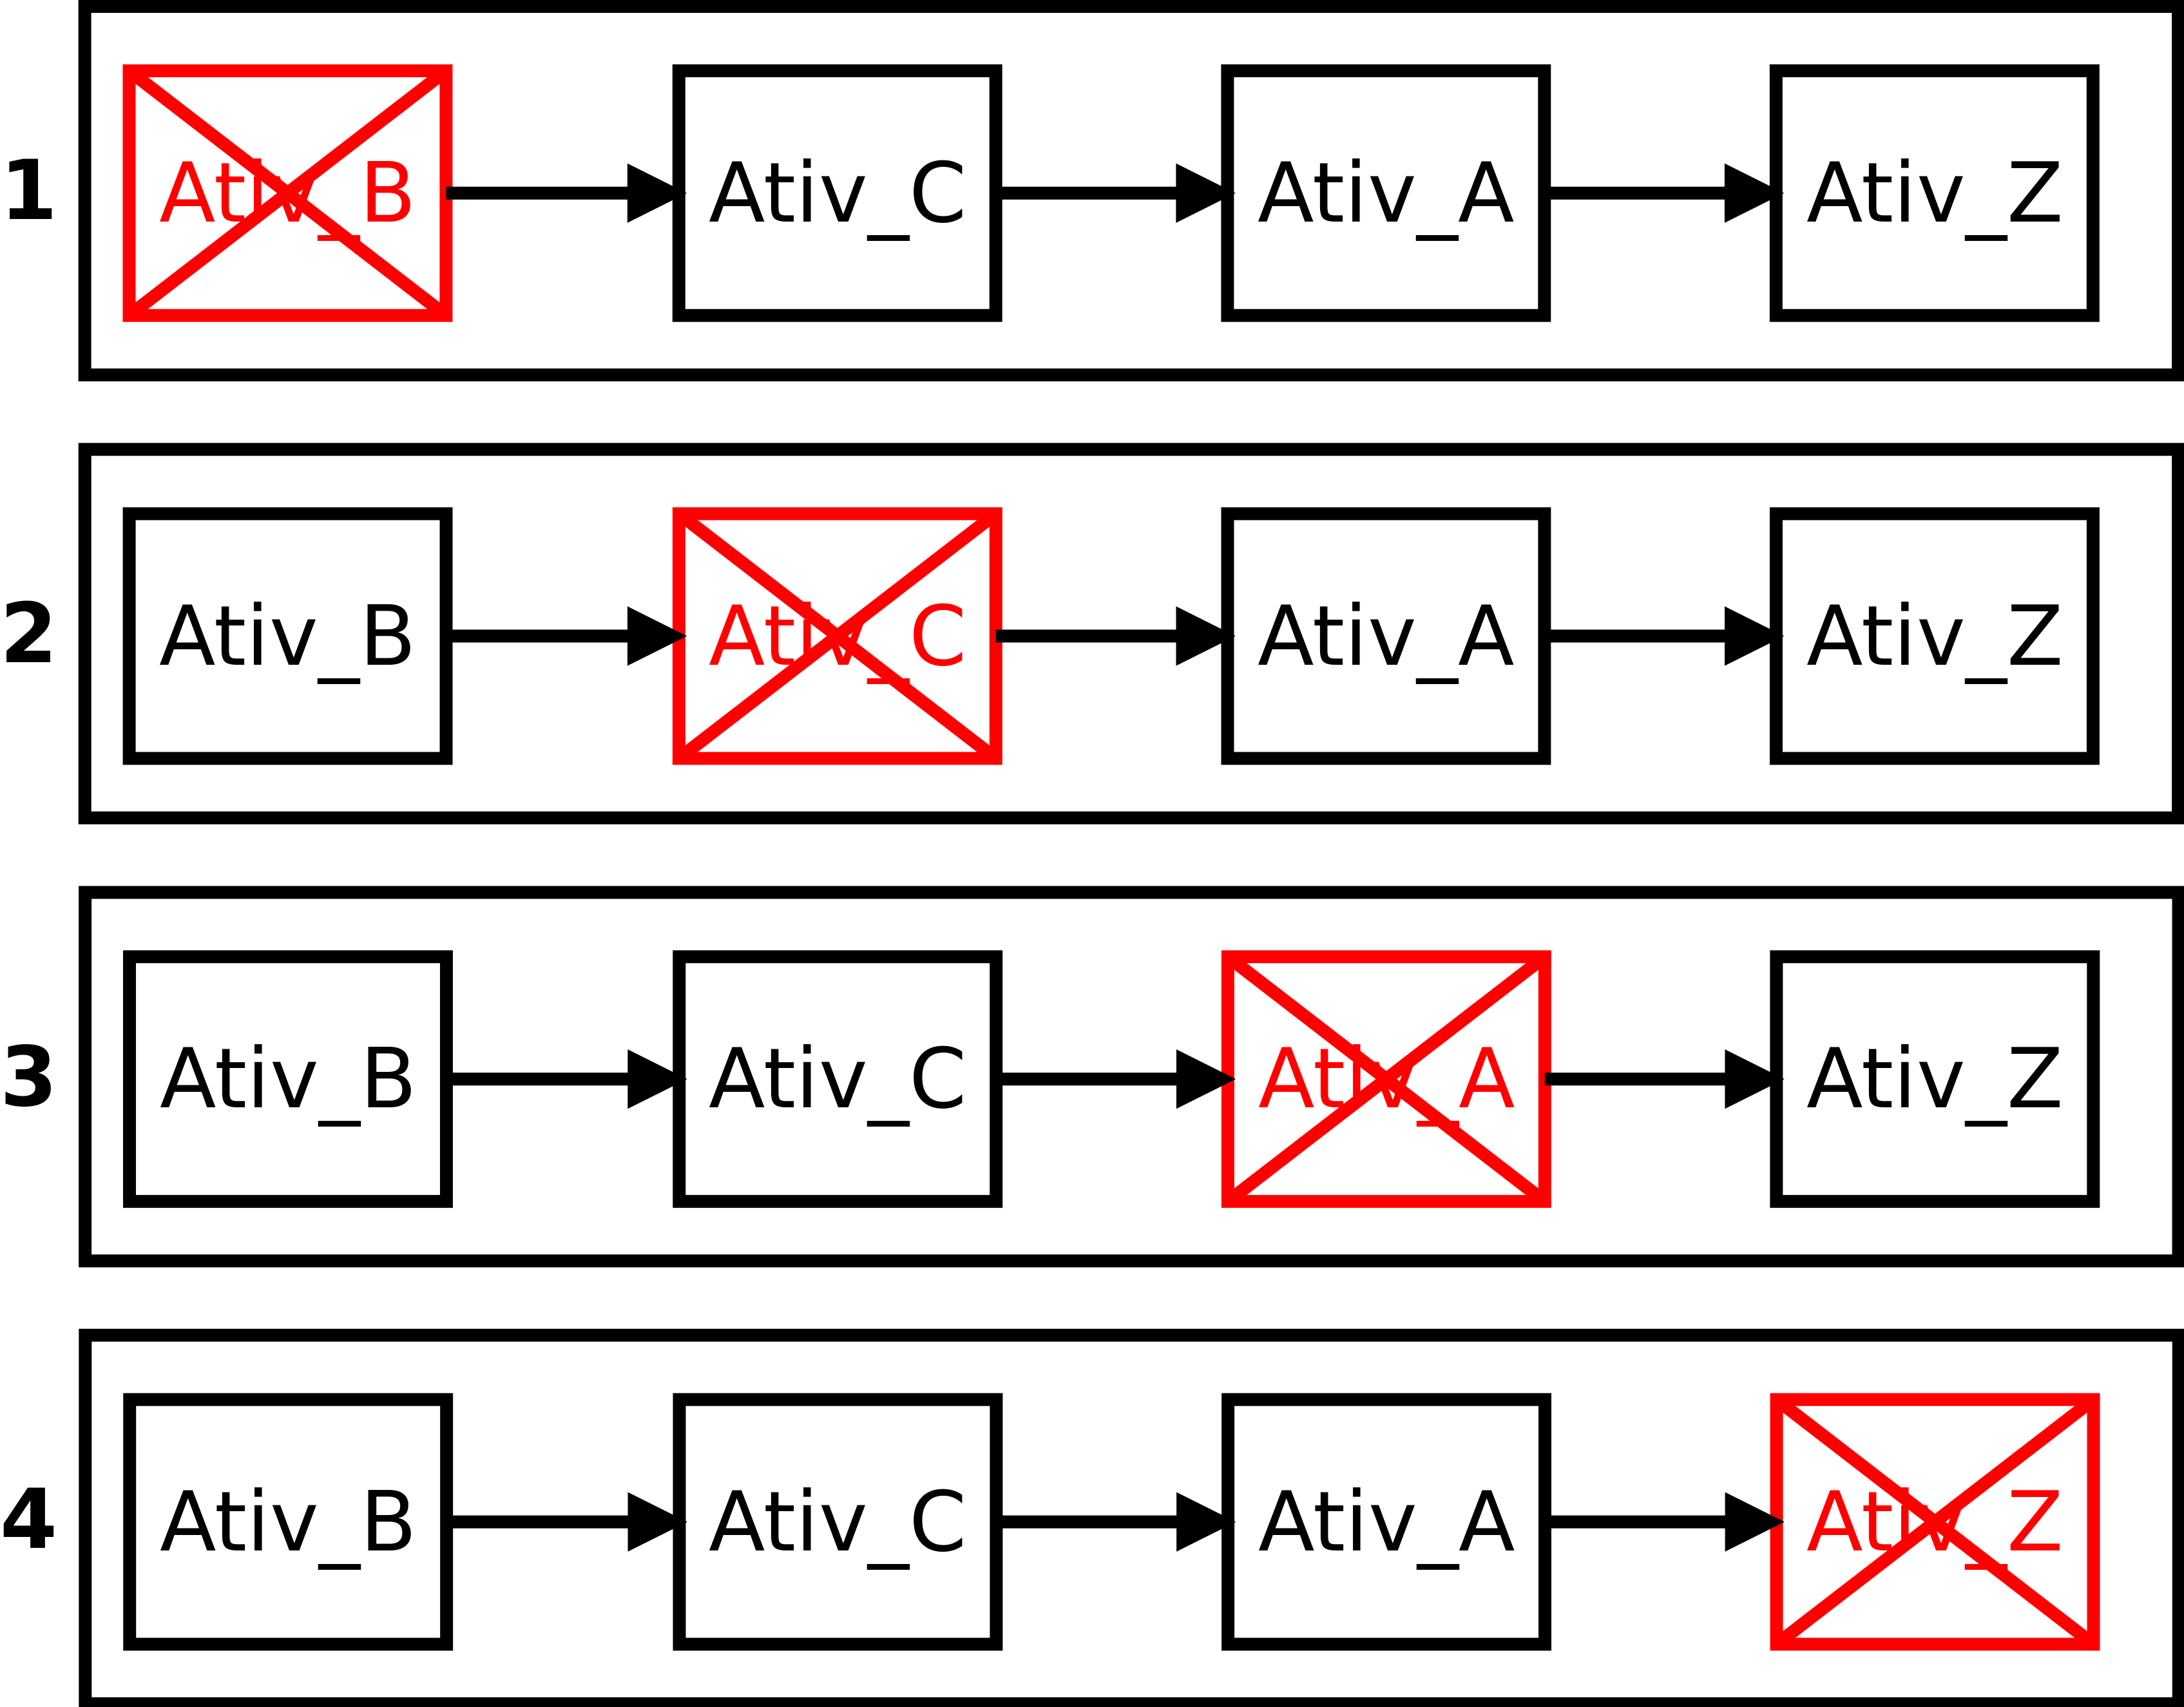
\includegraphics[width=10cm, height=5cm]{./secoes/conceitosFundamentais/pics/img/atividadeRemovida.png}
    \source{\varAutorData.}
	\label{figura_atividades_removidas}
\end{figure}

As Tabelas \ref{TABELAO:SISTEMA_RECOMENDACAO_01}, \ref{TABELAO:SISTEMA_RECOMENDACAO_02}, \ref{TABELAO:SISTEMA_RECOMENDACAO_03} e \ref{TABELAO:SISTEMA_RECOMENDACAO_04} apresentam os resultados dos quatro sistemas de recomendação. Cada item em negrito das listas representa a atividade que foi removida do workflow (que é o item considerado correto), ver Figura \ref{figura_atividades_removidas}, sua posição é determinada na coluna \emph{Rank}.
\begin{table}[!htbp]
\tiny
 \caption{Exemplo de recomendações de atividades usando quatro sistemas de recomendação.}
   \begin{subtable}{.5\linewidth}
    	\centering
   		\begin{tabular}{cllll} \hline 
   		\textbf{Rank} & \textbf{Lista} \(\mathbf{01}\) & \textbf{Lista} \(\mathbf{02}\) & \textbf{Lista} \(\mathbf{03}\) & \textbf{Lista} \(\mathbf{04}\) \\ \hline 
   		1                & Ativ\_A	     		& Ativ\_H    			& Ativ\_Z   		& Ativ\_I    		\\
   		2                & \textbf{Ativ\_B}		& Ativ\_B   			& Ativ\_E   		& Ativ\_C 			\\
   		3                & Ativ\_C    			& Ativ\_I    			& \textbf{Ativ\_A}  & Ativ\_Z  			\\
   		4                & Ativ\_D   			& Ativ\_X    			& Ativ\_X    		& Ativ\_B			\\
   		5                & Ativ\_E   			& Ativ\_A			 	& Ativ\_C    		& Ativ\_S			\\
   		6                & Ativ\_F   			& Ativ\_D    			& Ativ\_D    		& Ativ\_N			\\
   		7                & Ativ\_G   			& \textbf{Ativ\_C}  	& Ativ\_Q    		& Ativ\_K			\\
   		8                & Ativ\_H   			& Ativ\_Z    			& Ativ\_B   		& \textbf{Ativ\_Z}	\\
   		9                & Ativ\_I    			& Ativ\_P   			& Ativ\_F   		& Ativ\_H			\\
   		10               & Ativ\_Z   			& Ativ\_F    			& Ativ\_K    		& Ativ\_A			\\ \hline
   		\end{tabular}
   		\caption{Sistema de recomendação \(01\).}   
   		\label{TABELAO:SISTEMA_RECOMENDACAO_01}		
   \end{subtable}%
   \begin{subtable}{.5\linewidth}
   		\centering
   		\begin{tabular}{cllll} \hline 
   		\textbf{Rank} & \textbf{Lista} \(\mathbf{01}\) & \textbf{Lista} \(\mathbf{02}\) & \textbf{Lista} \(\mathbf{03}\) & \textbf{Lista} \(\mathbf{04}\) \\ \hline 
   		1                & Ativ\_A	     		& \textbf{Ativ\_C}		& \textbf{Ativ\_A}	& Ativ\_I                    \\
   		2                & \textbf{Ativ\_B} 	& Ativ\_B   			& Ativ\_E   		& Ativ\_C 	                 \\
   		3                & Ativ\_C    			& Ativ\_I    			& Ativ\_Z			& Ativ\_A                    \\
   		4                & Ativ\_D   			& Ativ\_X    			& Ativ\_X    		& \textbf{Ativ\_Z}           \\
   		5                & Ativ\_E			   	& Ativ\_A			  	& Ativ\_C    		& Ativ\_S	                 \\
   		6                & Ativ\_F   			& Ativ\_D    			& Ativ\_D    		& Ativ\_N                    \\
   		7                & Ativ\_G   			& Ativ\_H    			& Ativ\_Q    		& Ativ\_K	                 \\
   		8                & Ativ\_H   			& Ativ\_Z    			& Ativ\_B   		& Ativ\_U	                 \\
   		9                & Ativ\_I    			& Ativ\_P   			& Ativ\_F   		& Ativ\_H	                 \\
   		10               & Ativ\_Z   			& Ativ\_F    			& Ativ\_K    		& Ativ\_X	           \\ \hline
   		\end{tabular}
   		 \caption{Sistema de recomendação \(02\).}
   		 \label{TABELAO:SISTEMA_RECOMENDACAO_02}
   \end{subtable}
   \\ \\ \hfill 
   \begin{subtable}{.5\linewidth}
      		\centering
      		\begin{tabular}{cllll} \hline 
      		\textbf{Rank} & \textbf{Lista} \(\mathbf{01}\) & \textbf{Lista} \(\mathbf{02}\) & \textbf{Lista} \(\mathbf{03}\) & \textbf{Lista} \(\mathbf{04}\) \\ \hline 
      		1                & Ativ\_A			    & Ativ\_H    			& Ativ\_F   		& Ativ\_I                    \\
      		2                & Ativ\_G    			& Ativ\_B   			& Ativ\_E   		& Ativ\_C 	                 \\
      		3                & Ativ\_C    			& Ativ\_I    			& Ativ\_Z			& Ativ\_A                    \\
      		4                & Ativ\_D   			& Ativ\_X    			& Ativ\_X    		& Ativ\_B	                 \\
      		5                & Ativ\_E   			& Ativ\_A	  			& Ativ\_C    		& Ativ\_S	                 \\
      		6                & Ativ\_F   			& Ativ\_D    			& Ativ\_D    		& Ativ\_N                    \\
      		7                & \textbf{Ativ\_B}		& Ativ\_Q				& Ativ\_Q    		& \textbf{Ativ\_Z}           \\
      		8                & Ativ\_H   			& Ativ\_Z    			& Ativ\_B   		& Ativ\_U	                 \\
      		9                & Ativ\_I    			& Ativ\_P   			& \textbf{Ativ\_A}	& Ativ\_H	                 \\
      		10               & Ativ\_Z   			& \textbf{Ativ\_C}		& Ativ\_K    		& Ativ\_X           \\ \hline
      		\end{tabular}
      	\caption{Sistema de recomendação \(03\).}
      	\label{TABELAO:SISTEMA_RECOMENDACAO_03}
      \end{subtable}%
      \begin{subtable}{.5\linewidth}
         		\centering
         		\begin{tabular}{cllll} \hline 
         		\textbf{Rank} & \textbf{Lista} \(\mathbf{01}\) & \textbf{Lista} \(\mathbf{02}\) & \textbf{Lista} \(\mathbf{03}\) & \textbf{Lista} \(\mathbf{04}\) \\ \hline 
         		1                & Ativ\_A			    & Ativ\_H    			& Ativ\_Z   		& \textbf{Ativ\_Z}           \\
         		2                & Ativ\_Z    			& \textbf{Ativ\_C}		& Ativ\_E   		& Ativ\_C 	                 \\
         		3                & Ativ\_C    			& Ativ\_I    			& Ativ\_Z			& Ativ\_A                    \\
         		4                & Ativ\_D   			& Ativ\_X    			& Ativ\_X    		& Ativ\_B	                 \\
         		5                & Ativ\_E   			& Ativ\_A			  	& Ativ\_C    		& Ativ\_X 	         		 \\
         		6                & Ativ\_F   			& Ativ\_D    			& Ativ\_D    		& Ativ\_N                    \\
         		7                & Ativ\_G   			& Ativ\_C    			& Ativ\_Q    		& Ativ\_K	                 \\
         		8                & Ativ\_H   			& Ativ\_Z    			& Ativ\_B   		& Ativ\_U	                 \\
         		9                & Ativ\_I    			& Ativ\_P   			& \textbf{Ativ\_A}	& Ativ\_H	                 \\
         		10               & \textbf{Ativ\_B}  	& Ativ\_F    			& Ativ\_K    		& Ativ\_S		     \\ \hline
         		\end{tabular}
         	\caption{Sistema de recomendação \(04\).}
      		\label{TABELAO:SISTEMA_RECOMENDACAO_04}
         \end{subtable}
\label{TABELAO}
\source{\varAutorData.}
\end{table}
O sistema de recomendação \(01\), cujos resultados se encontram na Tabela \ref{TABELAO:SISTEMA_RECOMENDACAO_01}, apresenta os seguintes resultados de \(S@k\)
\begin{align}
S@1 &= \frac{1}{4}  \Big( (I_{L_{1}} = 0) + (I_{L_{2}} = 0) + (I_{L_{3}} = 0) + (I_{L_{4}} = 0) \Big)	=	0		\\
S@3 &= \frac{1}{4}  \Big( (I_{L_{1}} = 1) + (I_{L_{2}} = 0) + (I_{L_{3}} = 1) + (I_{L_{4}} = 0) \Big)	=	0.5		\\
S@5 &= \frac{1}{4}  \Big( (I_{L_{1}} = 1) + (I_{L_{2}} = 0) + (I_{L_{3}} = 1) + (I_{L_{4}} = 0) \Big)	=	0.5		\\
S@7 &= \frac{1}{4}  \Big( (I_{L_{1}} = 1) + (I_{L_{2}} = 1) + (I_{L_{3}} = 1) + (I_{L_{4}} = 0) \Big)	=	0.75	\\
S@10 &= \frac{1}{4} \Big( (I_{L_{1}} = 1) + (I_{L_{2}} = 1) + (I_{L_{3}} = 1) + (I_{L_{4}} = 1) \Big) 	=	1		
\end{align}
onde \(I_{L_{1}}\) é o resultado da função indicadora \eqref{equ_indicativa}. Para as métricas \(RR\) e \(MRR\) este recomendador apresentou os seguintes resultados
\begin{align}
RR_{L_{1}} &= \frac{1}{2}		\\
RR_{L_{2}} &= \frac{1}{7}		\\
RR_{L_{3}} &= \frac{1}{3}		\\
RR_{L_{4}} &= \frac{1}{8}		
\end{align}
e cuja média é dada por 
\begin{align}
MRR &= \frac{1}{4} \left( \frac{1}{2} + \frac{1}{7} + \frac{1}{3} + \frac{1}{8} \right) = 0.275297
\end{align}

O sistema de recomendação \(02\), cujos resultados se encontram na Tabela \ref{TABELAO:SISTEMA_RECOMENDACAO_02}, apresenta os seguintes resultados de \(S@k\)
\begin{align}
S@1 &= \frac{1}{4}  \Big( (I_{L_{1}} = 0) + (I_{L_{2}} = 1) + (I_{L_{3}} = 1) + (I_{L_{4}} = 0) \Big) =	0.5		\\
S@3 &= \frac{1}{4}  \Big( (I_{L_{1}} = 1) + (I_{L_{2}} = 1) + (I_{L_{3}} = 1) + (I_{L_{4}} = 0) \Big) =	0.75	\\
S@5 &= \frac{1}{4}  \Big( (I_{L_{1}} = 1) + (I_{L_{2}} = 1) + (I_{L_{3}} = 1) + (I_{L_{4}} = 1) \Big) =	1		\\
S@7 &= \frac{1}{4}  \Big( (I_{L_{1}} = 1) + (I_{L_{2}} = 1) + (I_{L_{3}} = 1) + (I_{L_{4}} = 1) \Big) =	1		\\
S@10 &= \frac{1}{4} \Big( (I_{L_{1}} = 1) + (I_{L_{2}} = 1) + (I_{L_{3}} = 1) + (I_{L_{4}} = 1) \Big) =	1		
\end{align}
e os seguintes resultado de \(MRR\)
\begin{align}
RR_{L_{1}} &= \frac{1}{2}		\\
RR_{L_{2}} &= \frac{1}{1}		\\
RR_{L_{3}} &= \frac{1}{1}		\\
RR_{L_{4}} &= \frac{1}{4}		
\end{align}
e cuja média é dada por 
\begin{align}
MRR &= \frac{1}{4} \left( \frac{1}{2} + \frac{1}{1} + \frac{1}{1} + \frac{1}{4} \right) = 0.687500
\end{align}

O sistema de recomendação \(03\), cujos resultados se encontram na Tabela \ref{TABELAO:SISTEMA_RECOMENDACAO_03}, apresenta os seguintes resultados de \(S@k\)
\begin{align}
S@1 &= \frac{1}{4}  \Big( (I_{L_{1}} = 0) + (I_{L_{2}} = 0) + (I_{L_{3}} = 0) + (I_{L_{4}} = 0) \Big) =	0		\\
S@3 &= \frac{1}{4}  \Big( (I_{L_{1}} = 0) + (I_{L_{2}} = 0) + (I_{L_{3}} = 0) + (I_{L_{4}} = 0) \Big) =	0		\\
S@5 &= \frac{1}{4}  \Big( (I_{L_{1}} = 0) + (I_{L_{2}} = 0) + (I_{L_{3}} = 0) + (I_{L_{4}} = 0) \Big) =	0		\\
S@7 &= \frac{1}{4}  \Big( (I_{L_{1}} = 1) + (I_{L_{2}} = 0) + (I_{L_{3}} = 0) + (I_{L_{4}} = 1) \Big) =	0.5		\\
S@10 &= \frac{1}{4} \Big( (I_{L_{1}} = 1) + (I_{L_{2}} = 1) + (I_{L_{3}} = 1) + (I_{L_{4}} = 1) \Big) =	1		
\end{align}
e os seguintes resultados de \(RR\)
\begin{align}
RR_{L_{1}} &= \frac{1}{7}		\\
RR_{L_{2}} &= \frac{1}{10}		\\
RR_{L_{3}} &= \frac{1}{9}		\\
RR_{L_{4}} &= \frac{1}{7}		
\end{align}
cuja média é dada por
\begin{align}
MRR &= \frac{1}{4} \left( \frac{1}{7} + \frac{1}{10} + \frac{1}{9} + \frac{1}{7} \right) = 0.124206
\end{align}

O sistema de recomendação \(04\), cujos resultados se encontram na Tabela \ref{TABELAO:SISTEMA_RECOMENDACAO_04}, apresenta os seguintes resultados de \(S@k\)
\begin{align}
S@1 &= \frac{1}{4}  \Big( (I_{L_{1}} = 0) + (I_{L_{2}} = 0) + (I_{L_{3}} = 0) + (I_{L_{4}} = 1) \Big)  =	0.25 \\
S@3 &= \frac{1}{4}  \Big( (I_{L_{1}} = 0) + (I_{L_{2}} = 1) + (I_{L_{3}} = 0) + (I_{L_{4}} = 1) \Big)	 =	0.5	 \\
S@5 &= \frac{1}{4}  \Big( (I_{L_{1}} = 0) + (I_{L_{2}} = 1) + (I_{L_{3}} = 0) + (I_{L_{4}} = 1) \Big)	 =	0.5	 \\
S@7 &= \frac{1}{4}  \Big( (I_{L_{1}} = 0) + (I_{L_{2}} = 1) + (I_{L_{3}} = 0) + (I_{L_{4}} = 1) \Big)	 =	0.5	 \\
S@10 &= \frac{1}{4} \Big( (I_{L_{1}} = 1) + (I_{L_{2}} = 1) + (I_{L_{3}} = 1) + (I_{L_{4}} = 1) \Big) =	1		
\end{align}
e os seguintes resultado de \(RR\)
\begin{align}
RR_{L_{1}} &= \frac{1}{10}		\\
RR_{L_{2}} &= \frac{1}{2}		\\
RR_{L_{3}} &= \frac{1}{9}		\\
RR_{L_{4}} &= \frac{1}{1}		
\end{align}
e cuja média é dada por 
\begin{align}
MRR &= \frac{1}{4} \left( \frac{1}{10} + \frac{1}{2} + \frac{1}{9} + \frac{1}{1} \right) = 0.427777
\end{align}
Ao comparar os quatro sistemas é possível constatar que o melhor é o número \(02\) pois apresenta o maior valor de \(MRR = 0.687500\) e os maiores valores observados de \(S@1 = 0.5\) e \(S@3 = 0.75\).

\section{Recomendação a partir de banco de dados de \emph{workflows}}\label{SEC_RECOMENDACAO_BASE_WORKFLOWS}
Uma estratégia para se recomendar atividades em um \emph{workflow} é a baseada nas suas atividades existentes. Neste tipo de estratégia, com base nas atividades existentes no \emph{workflow} atual (em construção) procura-se por atividades que foram úteis a \emph{workflows} existentes. Para isto, algum critério de proximidade entre \emph{workflows} ou entre atividades costuma ser utilizado. Nas próximas subseções algumas abordagens que usam banco de dados de \emph{workflows} são apresentadas.

\subsection{Recomendação a partir da última atividade}
Uma maneira de se recomendar atividades com base num banco de \emph{workflows} é sugerir ao usuário as atividades que costumam ser mais frequentemente utilizadas após a última atividade inserida pelo usuário. Esta estratégia assume que a sequência de atividades costuma ser conservada entre diferentes \emph{workflows}.

\subsection{Recomendação a partir de \emph{itemsets}}\label{AAPRIORI}
O algoritmo \emph{Apriori} \cite{Agrawal1994} pesquisa por \emph{itemsets} frequentes, que são aqueles que apresentem um suporte mínimo, em uma base de transações para tal usa uma estratégia de três fases iterativas. A primeira é a geração de itemsets candidatos de tamanho \(k\) usando os itemsets de tamanho \(k-1\), de acordo com a propriedade Apriori para aumentar as chances de gerar \emph{itemsets} frequentes devem ser criados apenas \emph{itemsets} que contenham \(k-2\) items em comum. A segunda fase é a poda, onde são pesquisados \emph{itemsets} que contenham subitemsets não frequentes, os quais são removídos do conjunto de \emph{itemsets} candidatos. A última fase é o cálculo de suporte, na qual cada candidato tem seu suporte calculado varrendo-se a base de dados uma vez, os que contenham suporte menor que o mínimo são removidos. 

Um caso especial desse algoritmo é a criação do \emph{itemset} para \(k = 1\), aqueles que contém apenas um item no conjunto. Dessa forma, não podem ser criados a partir de um conjunto de tamanho inferior como no caso geral apresentado anteriormente. Neste caso são criados todos os possíveis conjuntos unitários em seguida a base de dados é usada para calcular seus suportes, por fim são removidos os que não contém suporte mínimo \cite{HanKamber2011}.
\begin{table}[!htbp]
 \caption{Bases de dados disponíveis para o gerente do supermercado.}
   \begin{subtable}{.5\linewidth}
    	\centering
   		\begin{tabular}{ll} \hline 
   		\textbf{Produto} & \textbf{id}	\\ \hline 
   		Pão              & 1	   		\\
   		Leite            & 2			\\
   		Açucar           & 3   			\\
   		Papel Higiênico  & 4   			\\
   		Manteiga         & 5   			\\
   		Fralda           & 6   			\\
   		Cerveja          & 7   			\\
   		Refrigerante     & 8  			\\
   		Iogurte          & 9   			\\
   		Suco	         & 10			\\ \hline
   		\end{tabular}
   		\caption{Produtos da base de dados.}   
   		\label{TABAPRIORI:PRODUTOSMERCADO}		
   \end{subtable}%
   \begin{subtable}{.5\linewidth}
   		\centering
   		\begin{tabular}{cllll} \hline 
   		\textbf{TID} & \textbf{Items comprados}		\\ \hline 
   		101                & \{1, 3, 5\}			\\
   		102                & \{2, 1, 3, 7, 5\}	 	\\
   		103                & \{4, 9, 2, 1\}    		\\
   		104                & \{5, 2, 1, 3, 9\}   	\\
   		105                & \{1, 8, 6, 4, 3, 5\}	\\
   		106                & \{9, 2, 8\}  			\\ \hline
   		\end{tabular}
   		 \caption{Compras efetuadas no supermercado.}
   		 \label{TABAPRIORI:ITEMSETS}
   \end{subtable}
\label{TABAPRIORI}
\vspace{0.1cm}
\source{Adaptado de \citeonline{HanKamber2011}.}
\end{table}

Algumas definições essenciais para compreender o algoritmo são; i) \emph{itemsets}; ii) \emph{k-itemset}; iii) regra de associção; iv) suporte; e iv) confiança. Cada conjunto de items comprados da Tabela \ref{TABAPRIORI:ITEMSETS} é denominado \emph{itemset} \cite{HanKamber2011}. Um \emph{itemset} com \(k\) elementos é chamado de \emph{k-itemset}. Uma regra de associação é uma relação entre \emph{itemsets} e tem o formato \(A \rightarrow B\). Cada regra de associação tem um suporte dado por
\begin{align}
sup(A \rightarrow B) =  P(A \cup B)
\end{align}
e uma confiança calculada como
\begin{align}
conf(A \rightarrow B) =  \frac{sup(A \rightarrow B)}{sup(A)}
\end{align}
Uma regra de associação \(r\) é considerada interessante caso \(sup(r) > \alpha\) e \(conf(r) > \beta\). A propriedade \emph{Apriori} diz que para que um \emph{itemset} seja considerado frequente todos os \emph{itemsets} contidos nele também devem ser frequentes \cite{HanKamber2011}. 

\subsection{Agrupamento hierárquico}\label{HHIERARQUICO}
Outra forma de se utilizar um banco de \emph{workflows} para recomendar atividades é por meio do uso de agrupamentos, em que \emph{workflows} \emph{similares} são agrupados em um mesmo conjunto. Esta estratégia pode ser utilizada para recomendar uma atividade, por exemplo, por meio da identificação de a qual grupo o \emph{workflow} em desenvolvimento pertence e recomendando-se a atividade mais frequente desse grupo que ainda não exista nesse \emph{workflow}.
\begin{figure}[!htb]
    \centering  
    \caption{Estratégias de agrupamento hierárquico divisivo e aglomerativo.}
    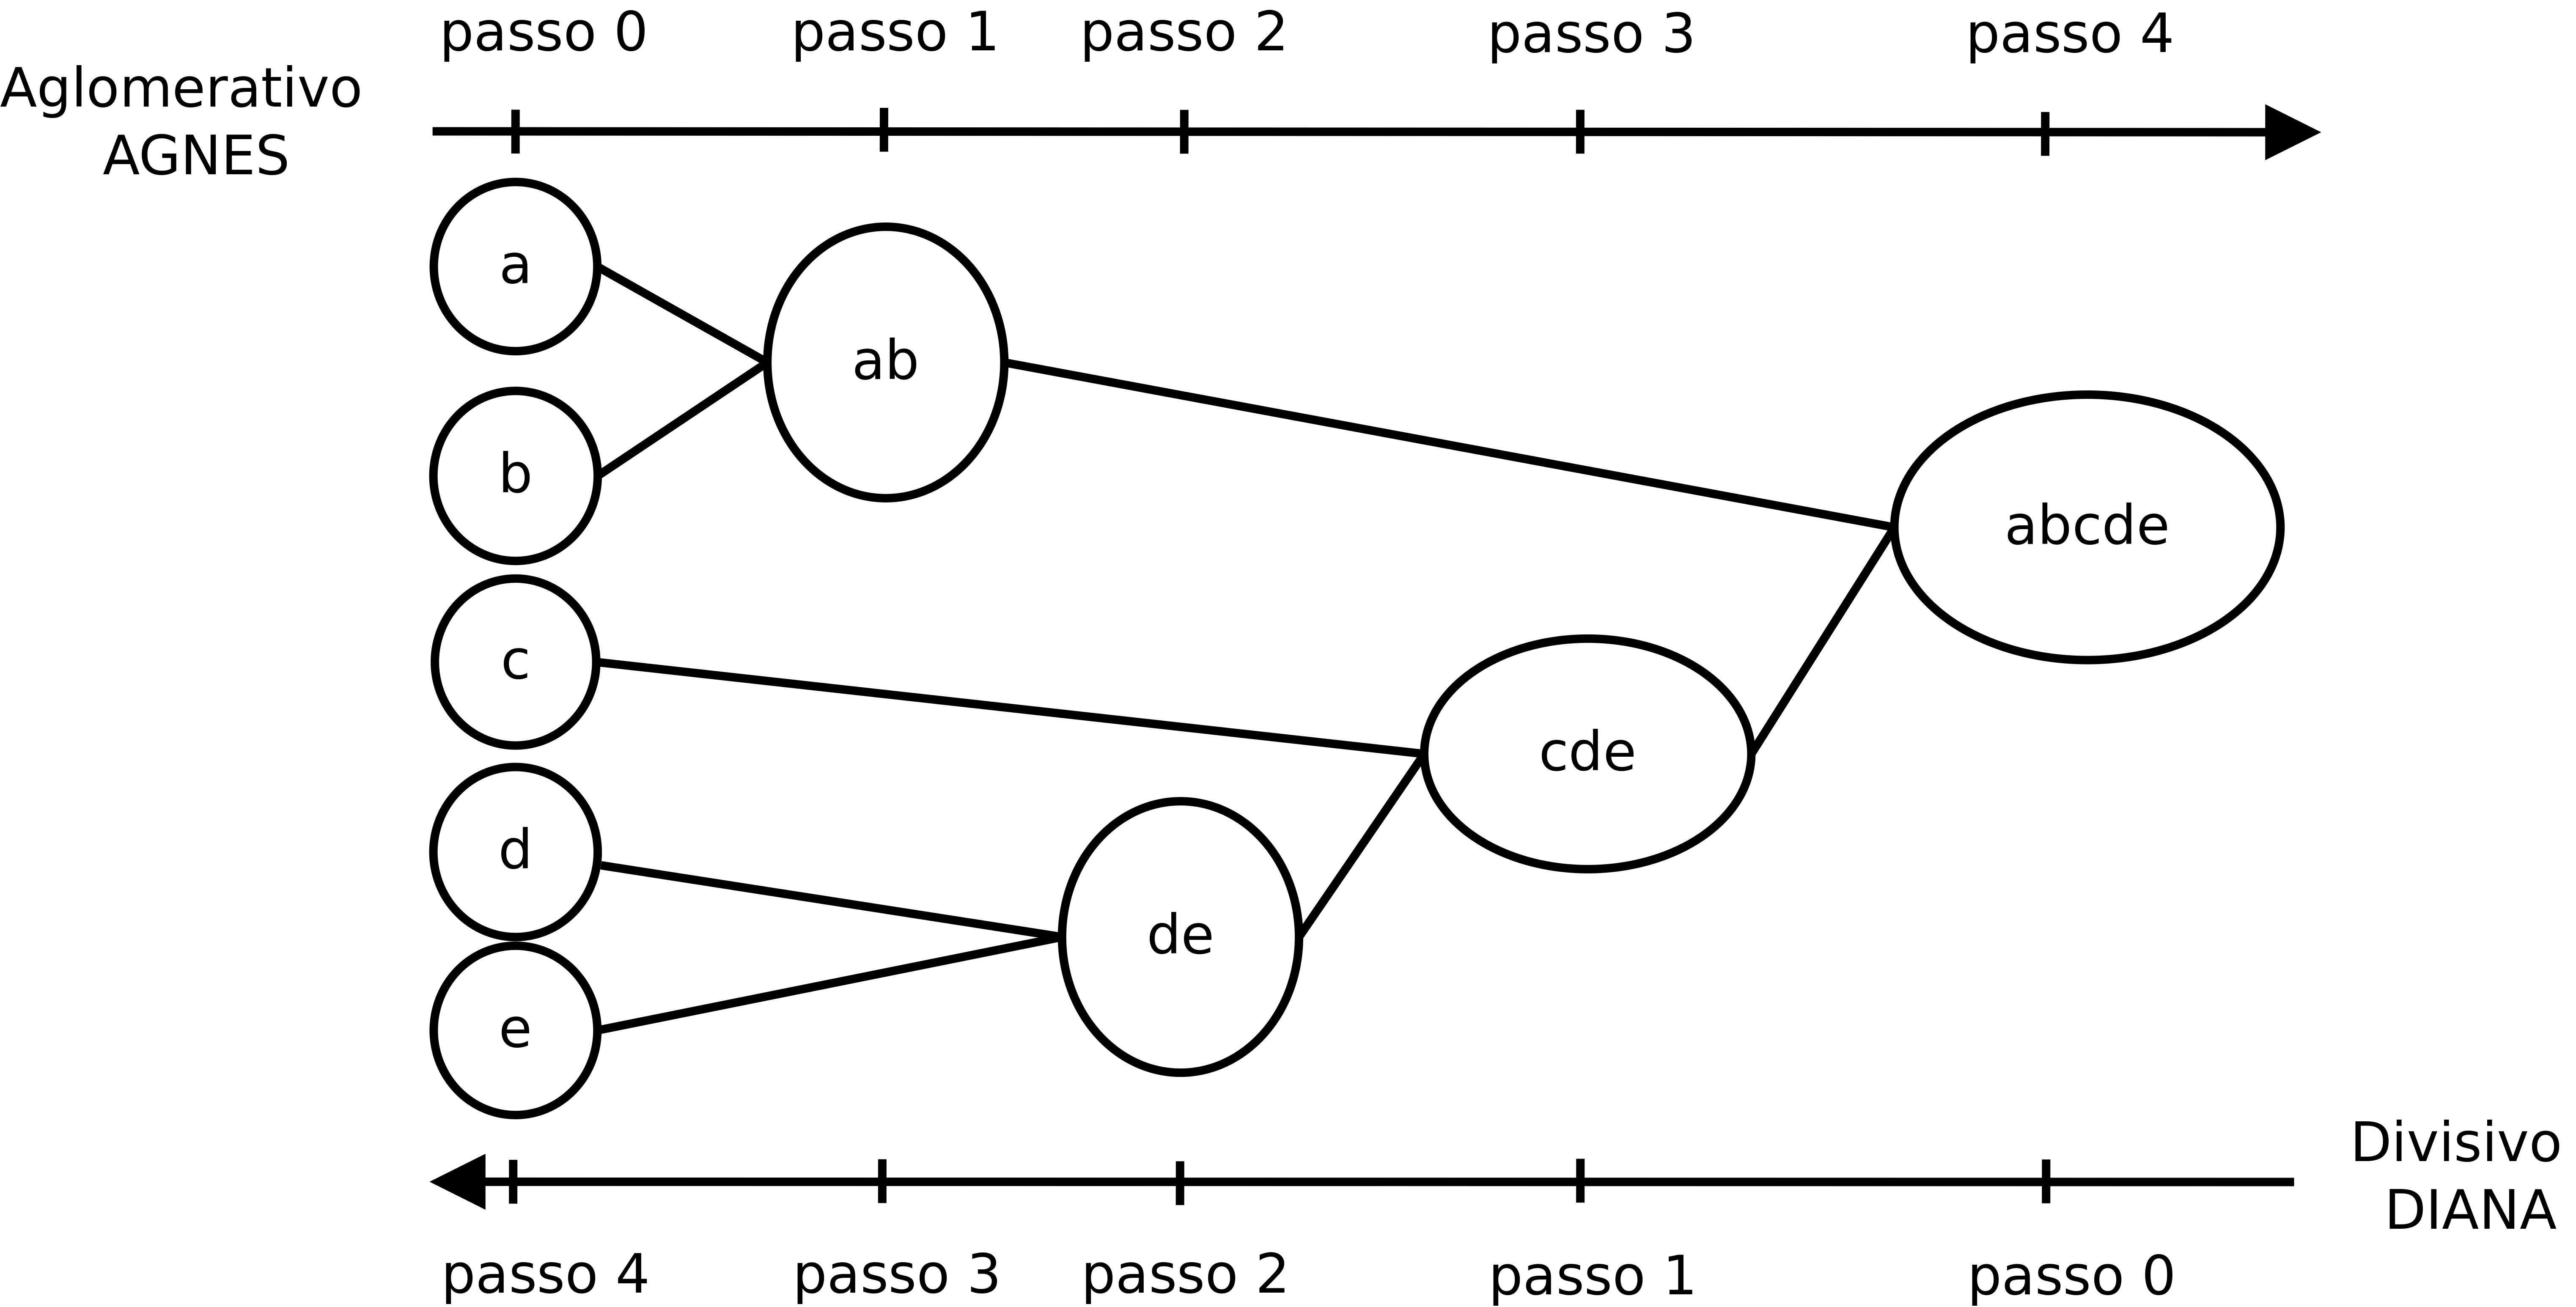
\includegraphics[width=13cm, height=7cm]{./secoes/conceitosFundamentais/pics/img/AGNES_DIANA.png}
     \source{Adaptado de \citeonline{HanKamber2011}.}
	\label{figura_exemplo_clusters}
\end{figure}

Existem diferentes formas de se agrupar dados, uma delas é o agrupamento agrupamento hierárquico. Algoritmos de agrupamento hierárquico agrupam dados em hierarquias ou árvores de agrupamentos \cite{HanKamber2011}, há duas abordagens para isto e ambas são exibidas na Figura \ref{figura_exemplo_clusters}. As divisivas, que iniciam com apenas um agrupamento contendo todos os dados e no decorrer do tempo subdivide-os até que cada agrupamento contenha apenas um dado como exibido no algoritmo DIANA \citeonline{Kaufman1990} apud \citeonline{HanKamber2011}. A outra abordagem é a aglomerativa, que inicia com vários agrupamentos, com apenas um dado cada e, com o decorrer do tempo, os agrupamentos são unidos até que exista apenas um cluster com todos os dados como o algoritmo AGNES na Figura \ref{figura_exemplo_clusters}.

%Não consegui acessar o artigo: Kaufman1990 :*(
O algoritmo \emph{AGlomerative NESting} (\emph{AGNES}) proposto por \citeonline{Kaufman1990} apud \citeonline{HanKamber2011} usa uma abordagem aglomerativa que atribuí um dado para cada agrupamento e em cada iteração aglomera dois agrupamentos segundo um critério a ser definido por exemplo, distância Euclidiana (ver seção \ref{SEC_SISTEMAS_RECOMENDACAO}).

Outro algoritmo hierárquico e aglomerativo, que consegue tratar dados categóricos, é o \emph{RObust Clustering using linKs} (ROCK) proposto por \citeonline {Sudipto2000}. Este algoritmo utiliza os conceitos de \emph{pontos vizinhos}, aqueles que são próximos segundo uma função de similaridade (\(sim(p_{i}, p_{j})\)), com um limiar \(\theta\) de similaridade mínima para ser considerado vizinho, e \emph{link} que é o número de vizinhos comuns entre pontos.

A cada iteração o algoritmo seleciona os melhores agrupamentos para união segundo a métrica de qualidade
\begin{align}
g(C_{i}, C_{j}) = \frac{link[C_{i}, C_{j}]}{(n_{i}+n_{j})^{1+2f(\theta)}-(n_{i})^{1+2f(\theta)}-(n_{j})^{1+2f(\theta)}}
\end{align}
onde \(n_{i}\) e \(n_{j}\) representam, respectivamente, o tamanho dos agrupamentos \(C_{i}\) e \(C_{j}\); \(link[C_{i}, C_{j}]\) corresponde ao número de vizinhos que os agrupamentos possuem em comum; e \(f(\theta)\) deve ser escolhida tal que \(n_{i}^{f(\theta)} \approx |C_{i}|\) e \(|C_{i}|\) número de objetos dentro do cluster \(i\).

O algoritmo seleciona uma amostra aleatória da base de dados, calcula o \emph{link} para os pares de pontos dessa amostra, no primeiro momento cada ponto representa um agrupamento, a cada iteração dois agrupamentos com maior qualidade são fundidos, até que exista apenas um, que contém todos os dados.

\section{Recomendação por classificação}\label{SEC_RECOMENDACAO_CLASSIFICACAO}
Segundo \citeonline{HanKamber2011} classificar itens computacionamente é construir um modelo que permita predizer suas classes discretas. O qual é construído em duas etapas a primeira é o treinamento, onde o classificador está aprendendo com um conjunto de itens rotulados. A segunda é a fase de testes, onde o classificador utiliza as regras aprendidas na fase anterior para classificar dados sem rótulo.

\subsection{KNN}
Na fase de treinamento este algoritmo determina quais são as classes de cada instância, usando alguma métrica de similaridade,  em seguida são apresentados os dados de teste. Cada instância de teste são localizados seus vizinhos mais próximos em seguida a instância é atribuída a classe do maior número de vizinhos (\(k\)) \cite{HanKamber2011}. Para exemplificar o funcionamento serão utilizados os dados da Tabela \ref{TAB_DADOS_EXEMPLO_KNN} como conjunto de treinamento.  
\begin{table}[h]
\center
\caption{Conjunto de treinamento (rotulado).}
\label{TAB_DADOS_EXEMPLO_KNN}
	
	\begin{tabular}{l c c c}
	\hline
		\textbf{alimento} & \textbf{doçura} & \textbf{crocância}  & \textbf{rótulo}   \\ \hline		
			uva 		& \(8\) & \(5\) & fruta  			\\ \hline
			feij{\~a}o  & \(3\) & \(7\) & vegetal 			\\ \hline
			castanha	& \(3\) & \(6\) & prote{\'i}na  	\\ \hline
			laranja 	& \(7\) & \(3\) & fruta  			\\ \hline	
	\end{tabular}
	\vspace{0.1cm}
	\source{Adaptado de \citeonline{MachineLearningwithR2013}.}
\end{table}

Será apresentado uma nova instância para o algoritmo KNN treinado com os dados da Tabela \ref{TAB_DADOS_EXEMPLO_KNN}, o Tomate que tem os atributos: i) doçura \( = 6\); e ii) crocância \( = 4\)). O algoritmo calcula as distâncias entre a instância \emph{tomate} e todos os dados de treinamento, como mostra a Figura \ref{FIGURA_KNN}, obtendo
\begin{align}
d(\mbox{uva},\mbox{tomate}) &= \sqrt{(6-8)^{2}+(4-5)^{2}} = 2.2		\\
d(\mbox{feijao},\mbox{tomate}) &= \sqrt{(6-3)^{2}+(4-7)^{2}} = 4.2	\\
d(\mbox{castanha},\mbox{tomate}) &= \sqrt{(6-3)^{2}+(4-6)^{2}} = 3.6	\\
d(\mbox{laranja},\mbox{tomate}) &= \sqrt{(6-7)^{2}+(4-3)^{2}} = 1.4									
\end{align}

Determinar a classe da instância \emph{tomate} depende do número \(k\) de vizinhos escolhidos pelo usuário e pelas distâncias calculadas. Utilizando \(k = 1\), a instância seria classificada como fruta, pois o único vizinho (laranja) pertence a este rótulo. Usando \(k = 3\), a instância terá três vizinhos: i) laranja; ii) uva; e iii) feijão; totalizando duas frutas e um vegetal consequentemente o tomate seria classificado como fruta novamente.
\begin{figure}[H]
	\centering
 	  \caption{Exemplo de classificação usando o algoritmo KNN.}
		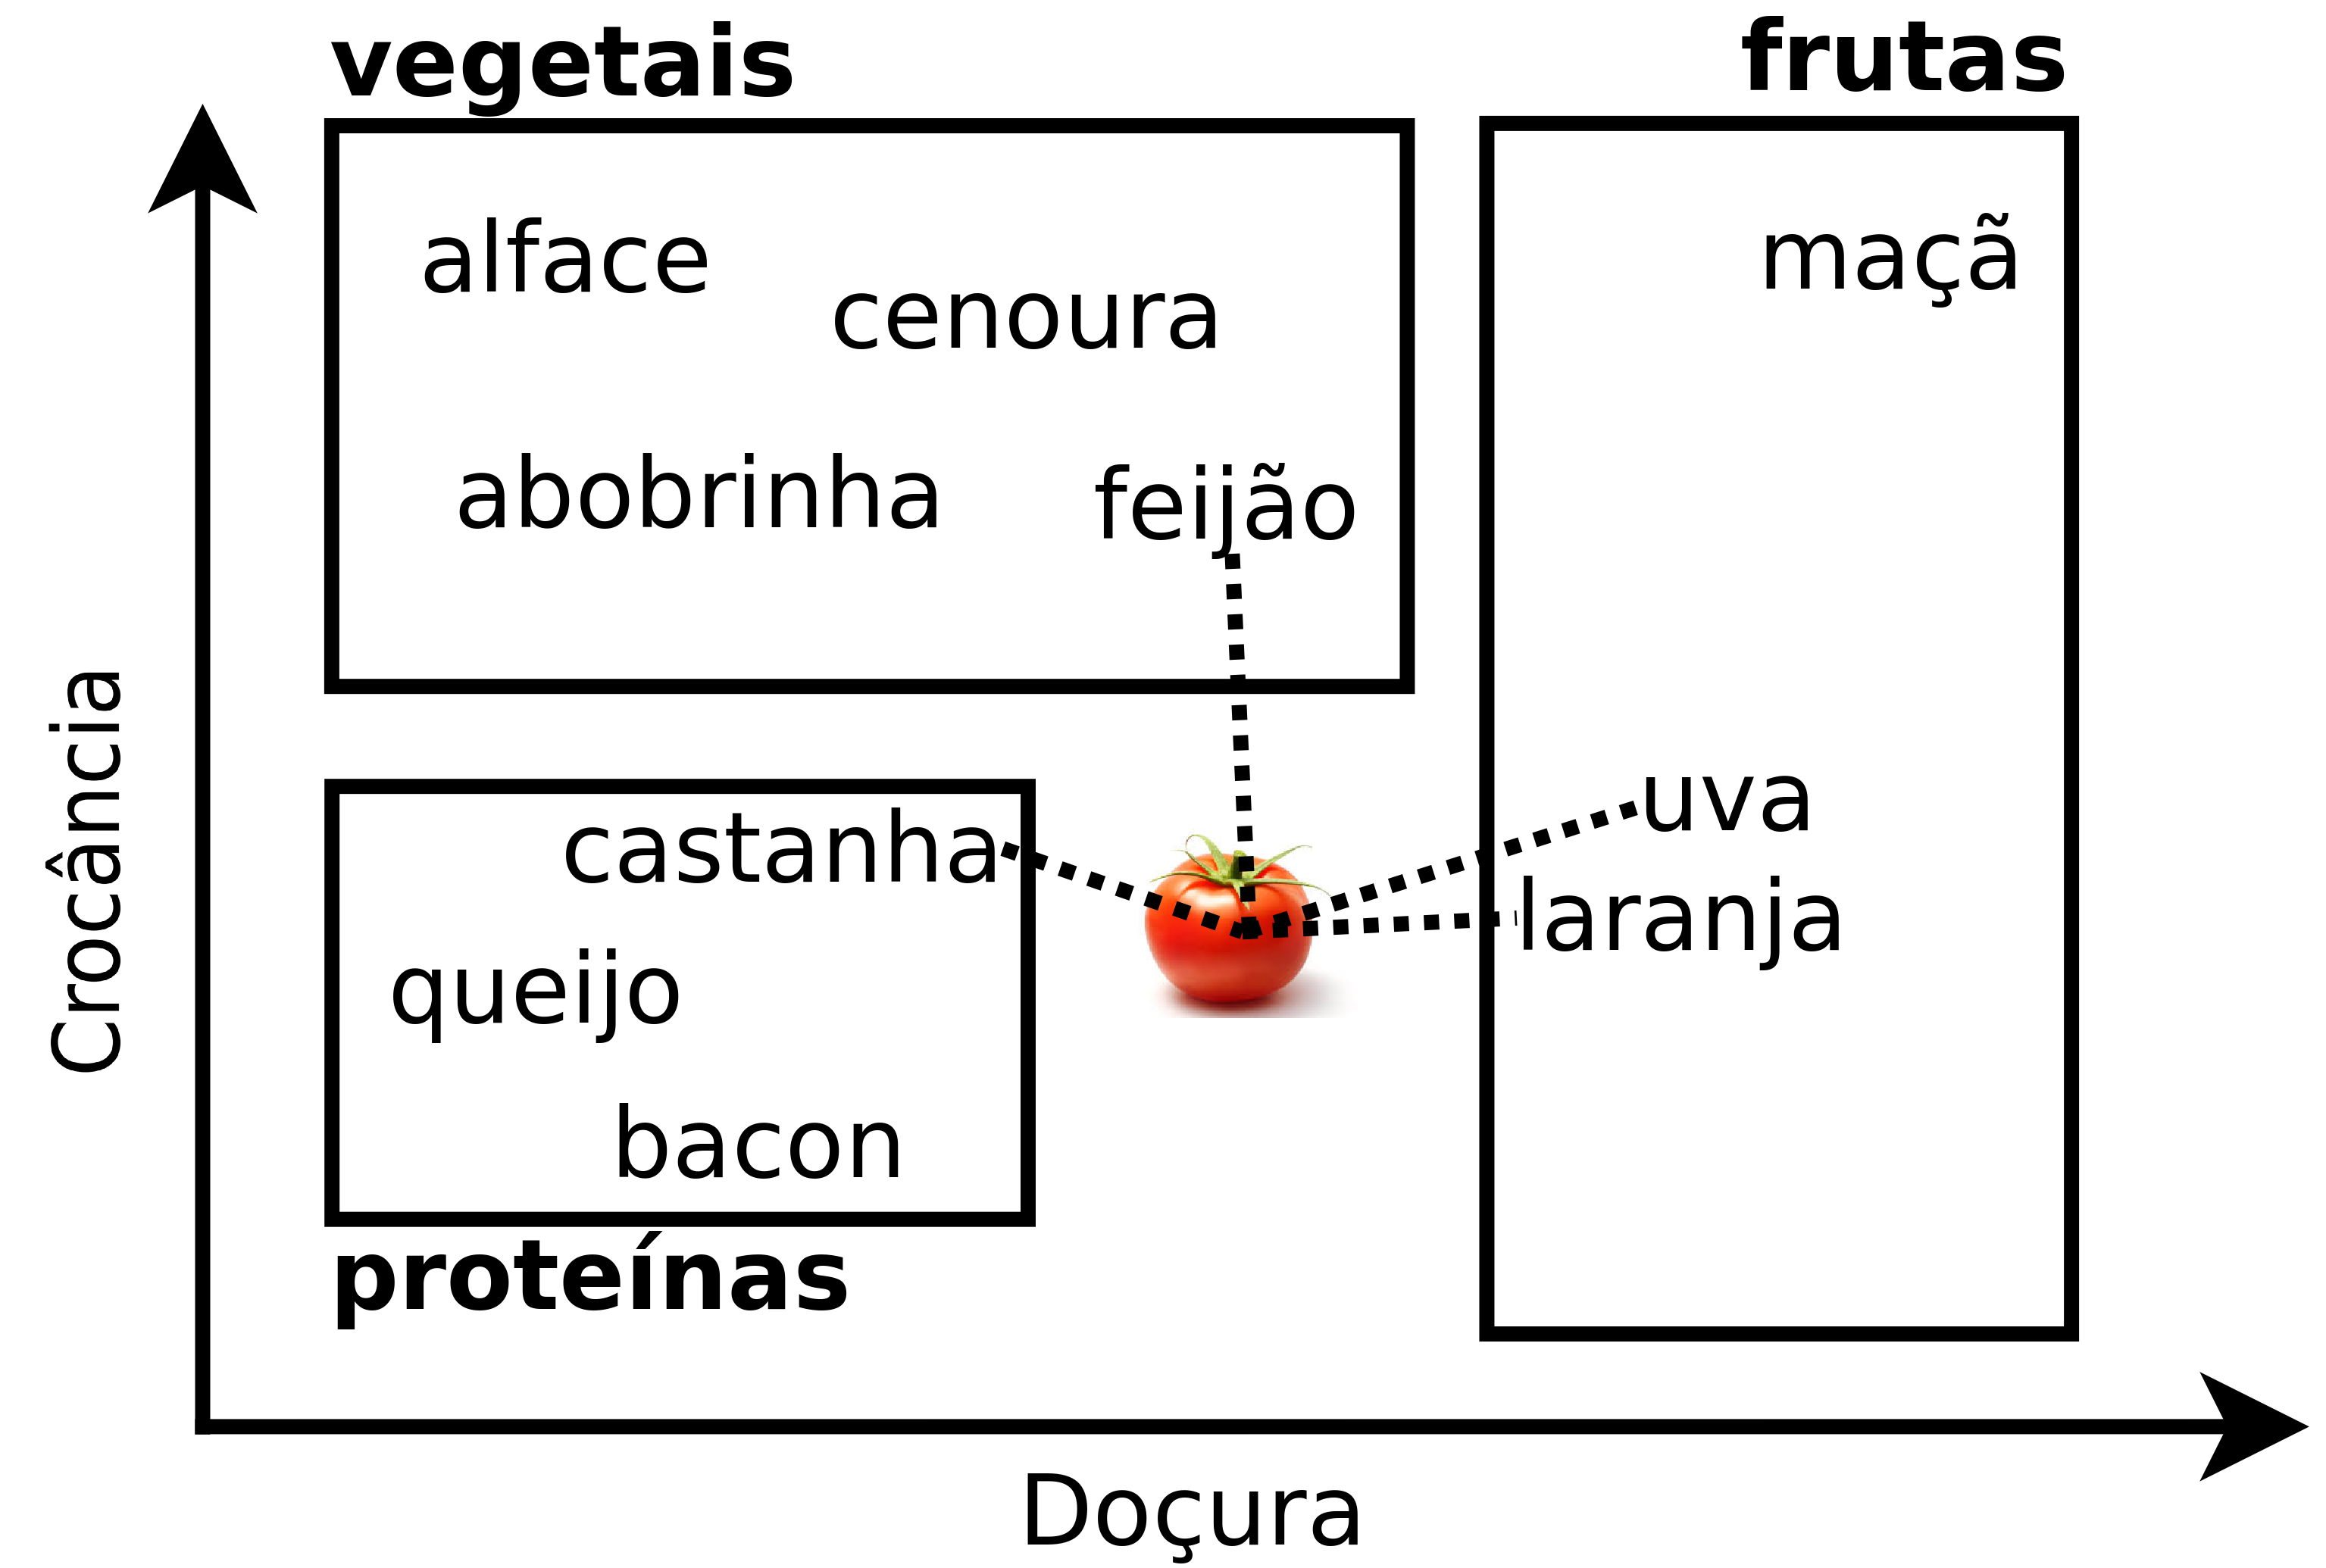
\includegraphics[width=11cm, height=6cm]{./secoes/conceitosFundamentais/pics/img/Tomate.png}
	\label{FIGURA_KNN}
  \source{Adaptado de \citeonline{MachineLearningwithR2013}.}
\end{figure}

Escolher um número de vizinhos usados para classificar (\(k\)) muito alto, causa uma redução no impacto de ruídos porém pode viesar o classificador tornando-o imcapaz de identificar padrões significativos. Em contrapartida, utilizar um valor  muito baixo, como \(k = 1\), pode tornar o algoritmo sensível demais e classificar os dados de acordo com ruídos.

Uma possível abordagem para encontrar um bom valor de \(k\) é testar o conjunto de dados para diversos valores e comparar as diferentes performances de classificação.

\subsection{Árvores de classificação e regressão - classificador e regressor}
Técnicas baseadas em árvores de decisão usam uma estrutura em árvore para tomar decisões, esta estrutura é constituída por um nó \emph{raiz}, diversos nós de \emph{decisão} e os nós \emph{folha}, como descritos na Figura \ref{FIGURA_ARVORE_DECISAO}. 

O aprendizado das árvores é feito utilizando o conjunto de treinamento, no qual é selecionado o atributo que maximiza algum critério de divisão (ver equações \eqref{EQ_Ganho_Ganho_Informacao} e \eqref{EQ_Gini_03}) responsável por particionar o conjunto. Este atributo pode se tornar um nó de \emph{decisão}, no caso das instâncias da partição criada por esta divisão conterem rótulos diferentes, ou um nó \emph{folha}, no caso das instâncias da partição criada por esta divisão conterem o mesmo rótulo \cite{HanKamber2011}.
\begin{figure}[H]
	\centering
 	  \caption{Estrutura de árvore de decisão.}
		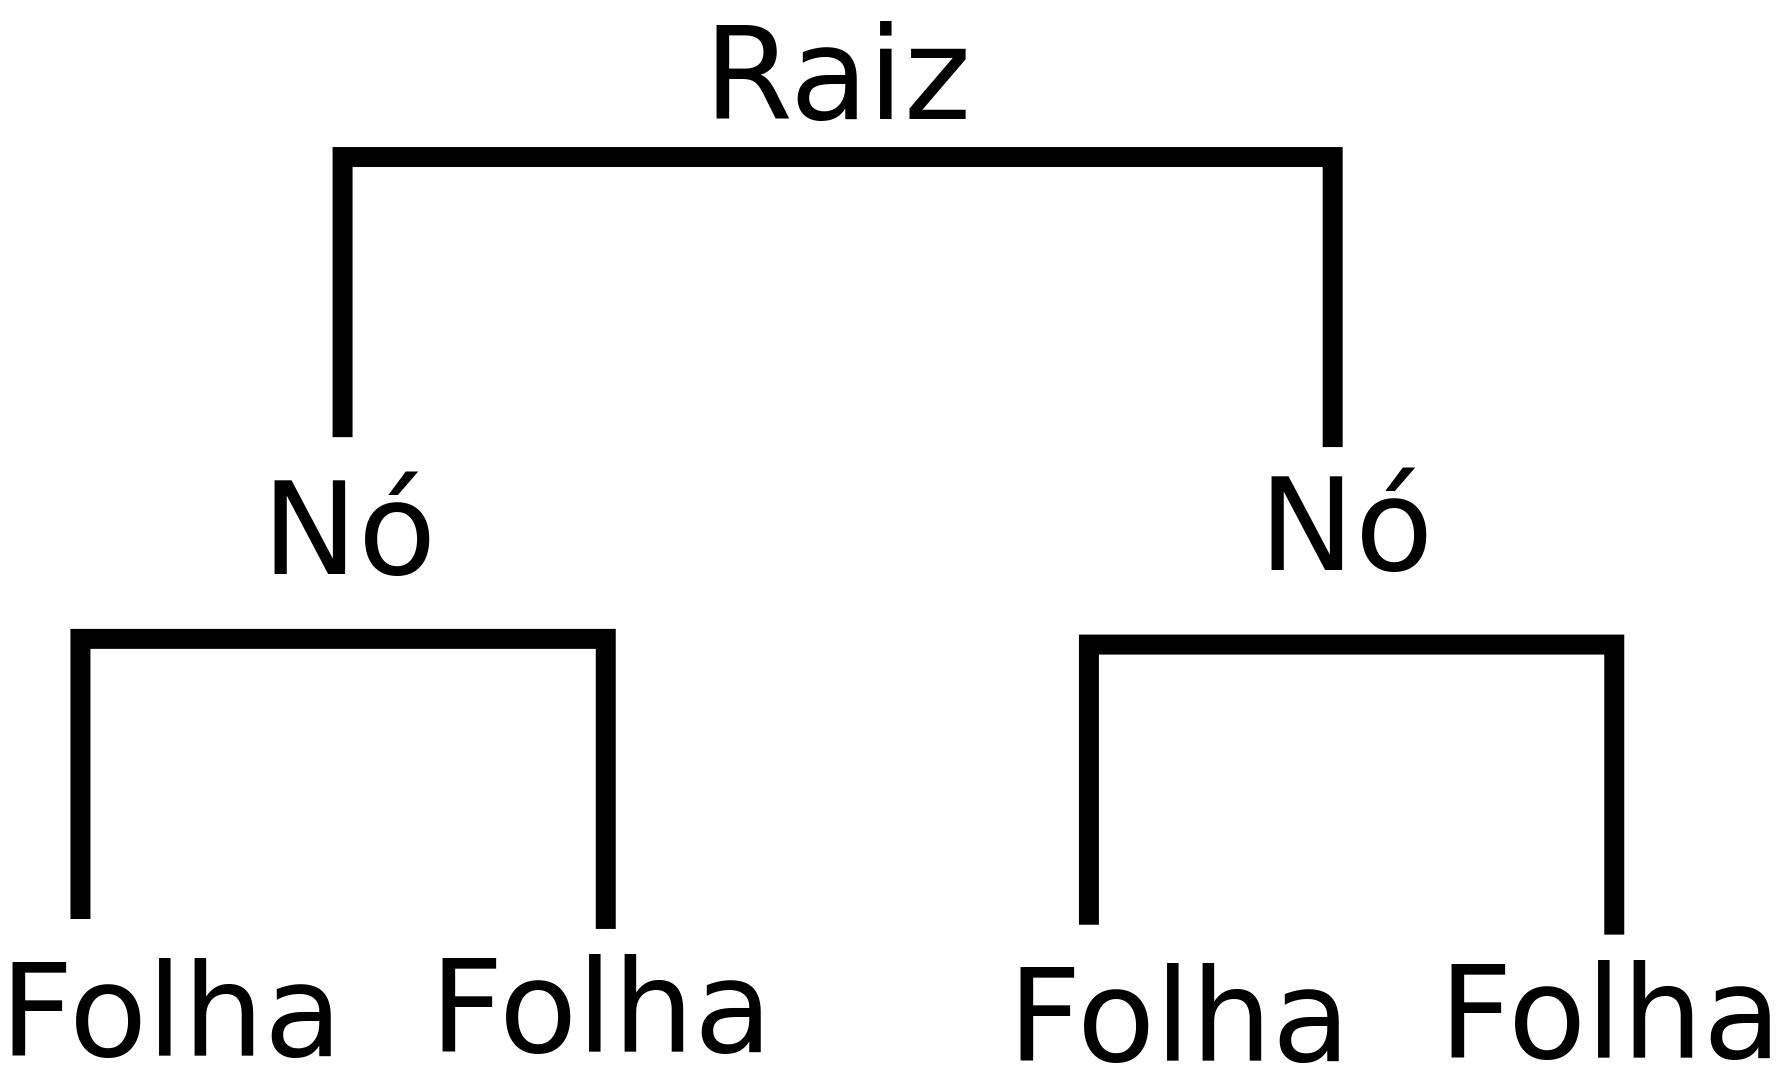
\includegraphics[width=5cm, height=4cm]{./secoes/conceitosFundamentais/pics/img/Arvore.png}
	\label{FIGURA_ARVORE_DECISAO}
  \source{Adaptado de \citeonline{Williams2011}.}
\end{figure}

O algoritmo CART proposto por \citeonline{Breiman1984} utiliza uma abordagem top-down que constrói a árvore recursivamente selecionando o melhor atributo baseado no índice de Gini (ver equação \eqref{EQ_Gini_03}) a cada iteração. O crescimento da árvore termina quando não há mais possibilidade de crescimento, o próximo passso é a poda que constrói \(k\) árvores de decisão onde \(T_{1}\) é identica a \(T_{0}\) com excessão de um ramo que se transformou em folha e \(T_{k}\) é apenas uma folha. É selecionada a melhor árvore com base no menor erro de classificação \cite{Breiman1984}. 

Alguns critérios de divisão muito utilizados para classificação em árvores de decisão são: i) entropia (da área da Física); e ii) o ganho de informação, conceito que deriva da teoria da informação. A entropia, metrifica o grau de incerteza em um conjunto, por exemplo um conjunto de dados com apenas um valor observado de classe tem entropia é zero. Outro conjunto que metade dos valores residem em uma classe e a outra metade em outra terá entropia máxima, o cálculo de entropia \cite{HanKamber2011} é descrito pelas seguintes equações
\begin{align}
Entropy(D) &= - \sum\limits_{i=1}^{m}p_{i}\log_{2}(p_{i})\label{EQ_Entropia_Ganho_Informacao} \\
Info_{A} &= \sum\limits_{i=1}^{N_{C}}\frac{D_{i}}{D}Entropy(D_{i})\label{EQ_Informacao_AtributoA_Ganho_Informacao}\\
Ganho(A) &= Info(D) - Info_{A}(D)\label{EQ_Ganho_Ganho_Informacao}
\end{align}
onde \(p_{i}\) é a probabilidade da classe \(C_{i}\) em \(D\) e \(Ganho(A)\) calcula o ganho de informação utilizando o atributo \(A\). Esse cálculo é aplicado em todos os atributos, é escolhido o que obtiver maior ganho de informação.

Outro critério que pode ser adotado para divisão é o índice de Gini \cite{HanKamber2011}, que mede a impureza de um conjunto de dados, o número de instâncias encontradas na partição que não pertencem a mesma classe, é calculada por:
\begin{align}
Gini(D) &= 1 - \sum\limits_{i=1}^{m}(p_{i})^{2}\label{EQ_Gini_01} \\
Gini_{A}(D) &= \sum\limits_{i=1}^{N_{C}}\frac{D_{i}}{D}Gi(niD_{i})\label{EQ_Gini_02} \\
\Delta Gini(A) &= Gini(D) - Gini_{A}(D)\label{EQ_Gini_03}
\end{align}
O atributo escolhido para teste lógico é aquele maximiza o \(\Delta Gini(A)\), em outras palavras, reduz a impureza do conjunto. Esses critérios são usados para particionar os conjuntos de dados de forma recorrente até que se atinja um critério de parada, determinado pelo algoritmo. 

Para tarefas de regresão o algoritmo tem algumas diferenças. A primeira é usar como métrica de impureza a soma residual ao quadrado (SRQ), definida por
\begin{align}
\operatorname*{arg\,min}_{x_{j} \leq x_{j}^{R}} \qquad [P_{l}Var(Y_{l}) + P_{r}Var(Y_{r})]
\end{align}
cujo objetivo desse problema é minimizar a soma da probabilidade da variância dos nós filhos gerados após uma divisão. Outra diferença é que cada nó \emph{folha} será preenchido pela média dos valores das instâncias de treinamento atribuídos naquela folha. E por fim, supõe uma relação linear entre a variável resposta e os preditores. Outros aspectos como construção, poda e treinamento são idênticos a árvores de classificação \cite{Connor2007}.


\subsection{Naive Bayes}
Classificadores baseados em técnicas Bayesianas utilizam os dados treinados para calcular a probabilidade observada de cada classe de acordo com suas características. Esses classificadores são melhor aplicados em problemas onde a informação de vários atributos pode ser considerada simultaneamente para gerar uma estimativa de probabilidades de saídas.

O algoritmo \emph{Naive Bayes} é uma técnica Bayesiana, que é uma aplicação do teorema de Bayes adaptado para classificação, que assume as condições ingênuas sobre os dados: i) independência de características; e ii) que todas as características são igualmente importantes. No mundo real essas condições são falhas mas ainda assim o algoritmo possuí um desempenho satisfatório \cite{HanKamber2011}.

Para explicar o funcionamento da classificação por Naive Bayes será usado um exemplo adaptado de \citeonline{MachineLearningwithR2013}. O objetivo deste é construir um classificador binário de emails em: i) spam ; e ii) não spam; para tal são calculadas as probabilidades de ser spam e de não ser spam, usando o conjunto de dados de treinamento, e o email é classificado de acordo com a maior probabilidade. 

O classificador verifica se o email contém as seguintes palavras \emph{viagra} (\(W_{1}\)), \emph{dinheiro} (\(W_{2}\)), \emph{cancelar assinatura} (\(W_{3}\)) e \emph{comestíveis} (\(W_{4}\)) e aplica o teorema de Bayes. Suponha que o classificador deva rotular a mensagem \(M_{1}\) que contém as palavras: \emph{Viagra} e \emph{cancelar assinatura}, para tal usa-se a equação
\begin{align}
P(Spam|W_{1} \cap \neg W_{2} \cap \neg W_{3} \cap W_{4}) = \frac{(W_{1} \cap \neg W_{2} \cap \neg W_{3} \cap W_{4})P(Spam)}{(W_{1} \cap \neg W_{2} \cap \neg W_{3} \cap W_{4})} \label{aplicandoBayesEmail}
\end{align}
Os valores usados para cálculo das probabilidades são obtidos pelo conjunto de treinamento (rotulado) usado para treinar o algoritmo. Dado que a equação \eqref{aplicandoBayesEmail} é computacionalmente custosa o algoritmo Naive Bayes simplifica a sua complexidade computacional assumindo a independência de eventos de mesma classe, dada por
\begin{align}
P(A \cap B) = P(A)P(B)
\end{align}
o que permite simplificar (a complexidade computacional) da equação \eqref{aplicandoBayesEmail}, dada esta simplificação a probabilidade de um email ser classificado como \emph{spam} é dada por
\begin{align}
EvSpam &= Spam|W_{1} \cap \neg W_{2} \cap \neg W_{3} \cap W_{4} \\
P(EvSpam) &= \frac{P(W_{1}|Spam) P(\neg W_{2}|Spam) }{P(W_{1}) P(\neg W_{2})} \frac{P(\neg W_{3}|Spam) P(W_{4}|Spam) P(Spam)}{P(\neg W_{3}) P(W_{4})} \label{ProbabilidadeSpamBayes}
\end{align}
aplicando-se a fórmula simplificada novamente, obten-se a probabilidade do email ser classificado como \emph{não spam}, a qual é dada por
\begin{align}
\overline{EvSpam} &= \overline{Spam}|W_{1} \cap \neg W_{2} \cap \neg W_{3} \cap W_{4} \\
P(\overline{EvSpam}) &= \frac{P(W_{1}|\overline{Spam}) P(\neg W_{2}|\overline{Spam}) }{P(W_{1})  P(\neg W_{2})} \frac{P(\neg W_{3}|\overline{Spam}) P(W_{4}|\overline{Spam}) P(\overline{Spam})}{P(\neg W_{3}) P(W_{4})} \label{ProbabilidadeNaoSpamBayes}
\end{align}
Agora que foram definidas as probabilidade de uma mensagem ser spam (ou não spam), ver equações \eqref{ProbabilidadeSpamBayes} e \eqref{ProbabilidadeNaoSpamBayes}, serão utilizados os dados do conjunto de treinamento exibidos na Tabela \ref{tab_verossimilhancasExemploNaiveBayes} para calcular estas probabilidades e tomar uma decisão.
\bgroup
\def\arraystretch{1.5}
\begin{table}[!htp]
\centering
\caption{Verossimilhança do conjunto de treinamento.}
\begin{tabular}{|l|c|c|c|c|c|c|c|c|c|}
\hline
\multicolumn{1}{|c|}{} & \multicolumn{2}{c|}{$\mathbf{W_1}$} & \multicolumn{2}{c|}{$\mathbf{W_2}$} & \multicolumn{2}{c|}{$\mathbf{W_3}$} & \multicolumn{2}{c|}{$\mathbf{W_4}$} \\ \hline
Verossimilhança   &   Sim &   Não   &     Sim       &      Não      &     Sim       &       Sim &      Não      &      Sim                       \\ \hline

Spam   &   \(\frac{4}{20}\) &   \(\frac{16}{20}\)   &     \(\frac{10}{20}\)       &      \(\frac{10}{20}\)      &     \(\frac{0}{20}\)       &       \(\frac{20}{20}\)     &      \(\frac{12}{20}\)      &      \(\frac{8}{20}\)                       \\ \hline

Não Spam   &   \(\frac{1}{80}\) &   \(\frac{79}{80}\)   &     \(\frac{14}{80}\)       &      \(\frac{66}{80}\)      &     \(\frac{8}{80}\)       &       \(\frac{71}{80}\)     &      \(\frac{23}{80}\)      &      \(\frac{57}{80}\)                       \\ \hline
Total  &   \(\frac{5}{100}\) &   \(\frac{95}{100}\)   &     \(\frac{24}{100}\)       &      \(\frac{76}{100}\)      &     \(\frac{8}{100}\)       &       \(\frac{91}{100}\)     &      \(\frac{35}{100}\)      &      \(\frac{65}{100}\)                       \\ \hline
\end{tabular}
\vspace{0.1cm}
	\label{tab_verossimilhancasExemploNaiveBayes}
	\source{Adaptado de \citeonline{MachineLearningwithR2013}.}
\end{table}
\egroup

\noindent
Usando os dados da Tabela \ref{tab_verossimilhancasExemploNaiveBayes} e as equações \eqref{ProbabilidadeSpamBayes} e \eqref{ProbabilidadeNaoSpamBayes} obten-se
\begin{align}
& P(Spam|W_{1} \cap \neg W_{2} \cap \neg W_{3} \cap W_{4}) = \left(\frac{4}{20}\right) \left(\frac{10}{20}\right) \left(\frac{1}{20}\right) \left(\frac{12}{20}\right) \left(\frac{20}{100}\right) = 0.012 \\
& P(\overline{Spam}|W_{1} \cap \neg W_{2} \cap \neg W_{3} \cap W_{4}) = \left(\frac{1}{80}\right) \left(\frac{66}{80}\right) \left(\frac{71}{80}\right) \left(\frac{23}{80}\right) \left(\frac{80}{100}\right) = 0.002
\end{align}
A probabilidade de ser \emph{spam} é igual a verossimilhança de que a mensagem é \emph{spam} dividida pela probabilidade de ser \emph{spam} ou \emph{não spam}, logo obten-se
\begin{align}
P(Spam|W_{1} \cap \neg W_{2} \cap \neg W_{3} \cap W_{4}) = \frac{0.012}{0.012 + 0.002} = 0.857
\end{align}
De forma análoga para \emph{não spam} ten-se que
\begin{align}
P(\overline{Spam}|W_{1} \cap \neg W_{2} \cap \neg W_{3} \cap W_{4}) = \frac{0.002}{0.012 + 0.002} = 0.143 
\end{align}
Pode-se observar que a probabilidade da mensagem \(M_{1}\) ser \emph{spam} é maior que ser \emph{não spam}, logo será classificada como \emph{spam} pelo algoritmo Naive Bayes.

A teoria da probabilidade Bayesiana é a raiz para o cálculo de verossimilhança de um evento baseado em uma evidência, portanto serão revisados alguns conceitos básicos usados anteriormente. A probabilidade de um evento pode ser obtida pelos dados observados, dividindo o número de ocorrências de um evento pelo número total de dados. Dois eventos são ditos mutuamente exclusivos se eles não ocorrerem ao mesmo tempo. A Figura \ref{FIGURA_EVENTOS_MUTUAMENTE_EXCLUSIVOS} apresenta um exemplo de eventos mutuamente exclusivos.
\begin{figure}[H]
	\centering
 	  \caption{Eventos mutuamente exclusivos.}
		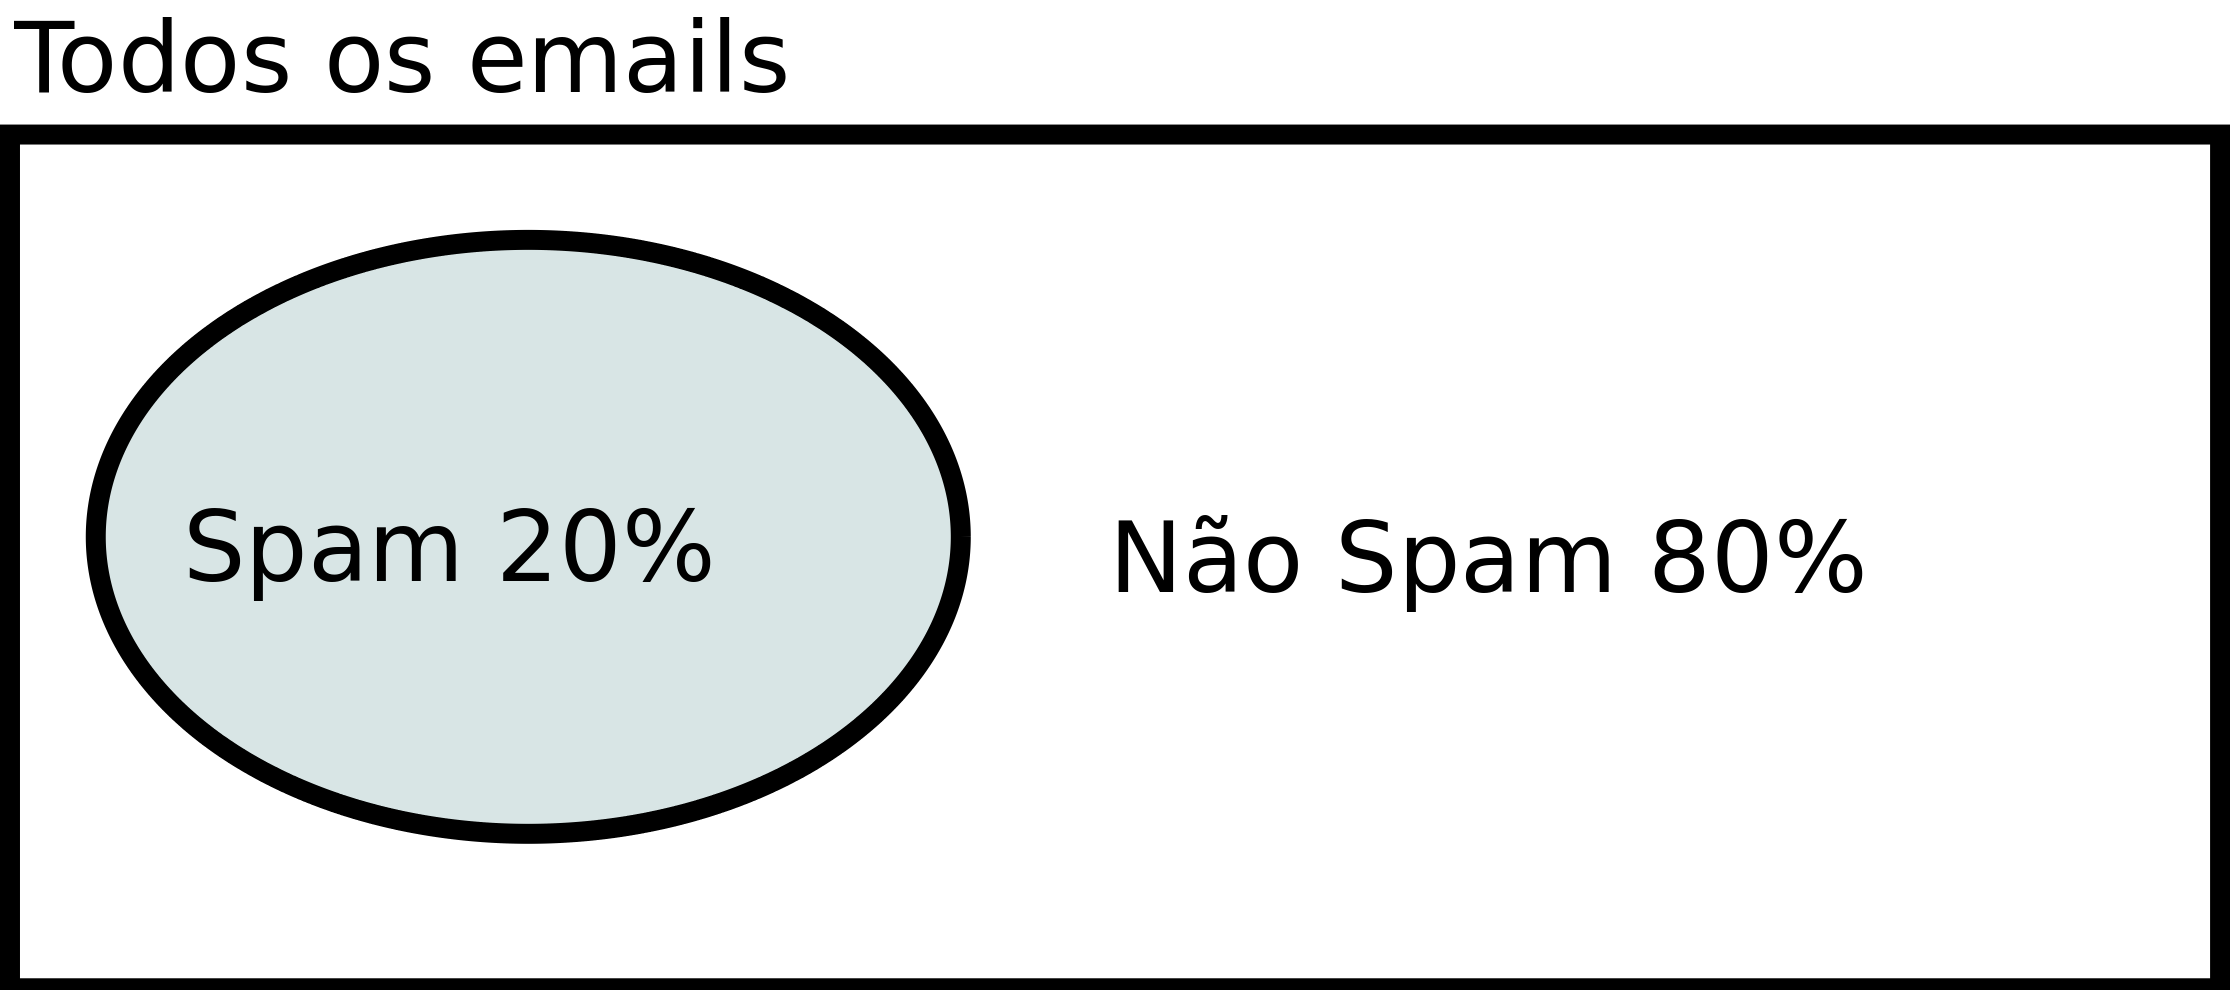
\includegraphics[width=7cm, height=4.5cm]{./secoes/conceitosFundamentais/pics/img/EventosMutuamenteExclusivos.png}
	\label{FIGURA_EVENTOS_MUTUAMENTE_EXCLUSIVOS}
  \source{Adaptado de \citeonline{MachineLearningwithR2013}.}
\end{figure}
Seja \(P(A)\) a probabilidade de um evento \(A\) ocorrer, e dados dois eventos mutuamente exclusivos \(A, B\) a seguinte relação é válida
\begin{align}
P(A) = 1 - P(B)
\end{align}

É comum estudar vários eventos não mutuamente exclusivos para a mesma saída, eventos que ocorrem em conjunto. Estes permitem que seja utilizado um evento para prever o outro. A Figura \ref{FIGURA_EVENTOS_NAO_MUTUAMENTE_EXCLUSIVOS} apresenta um exemplo de eventos não mutuamente exclusivos.
\begin{figure}[H]
	\centering
 	  \caption{Eventos não mutuamente exclusivos.}
		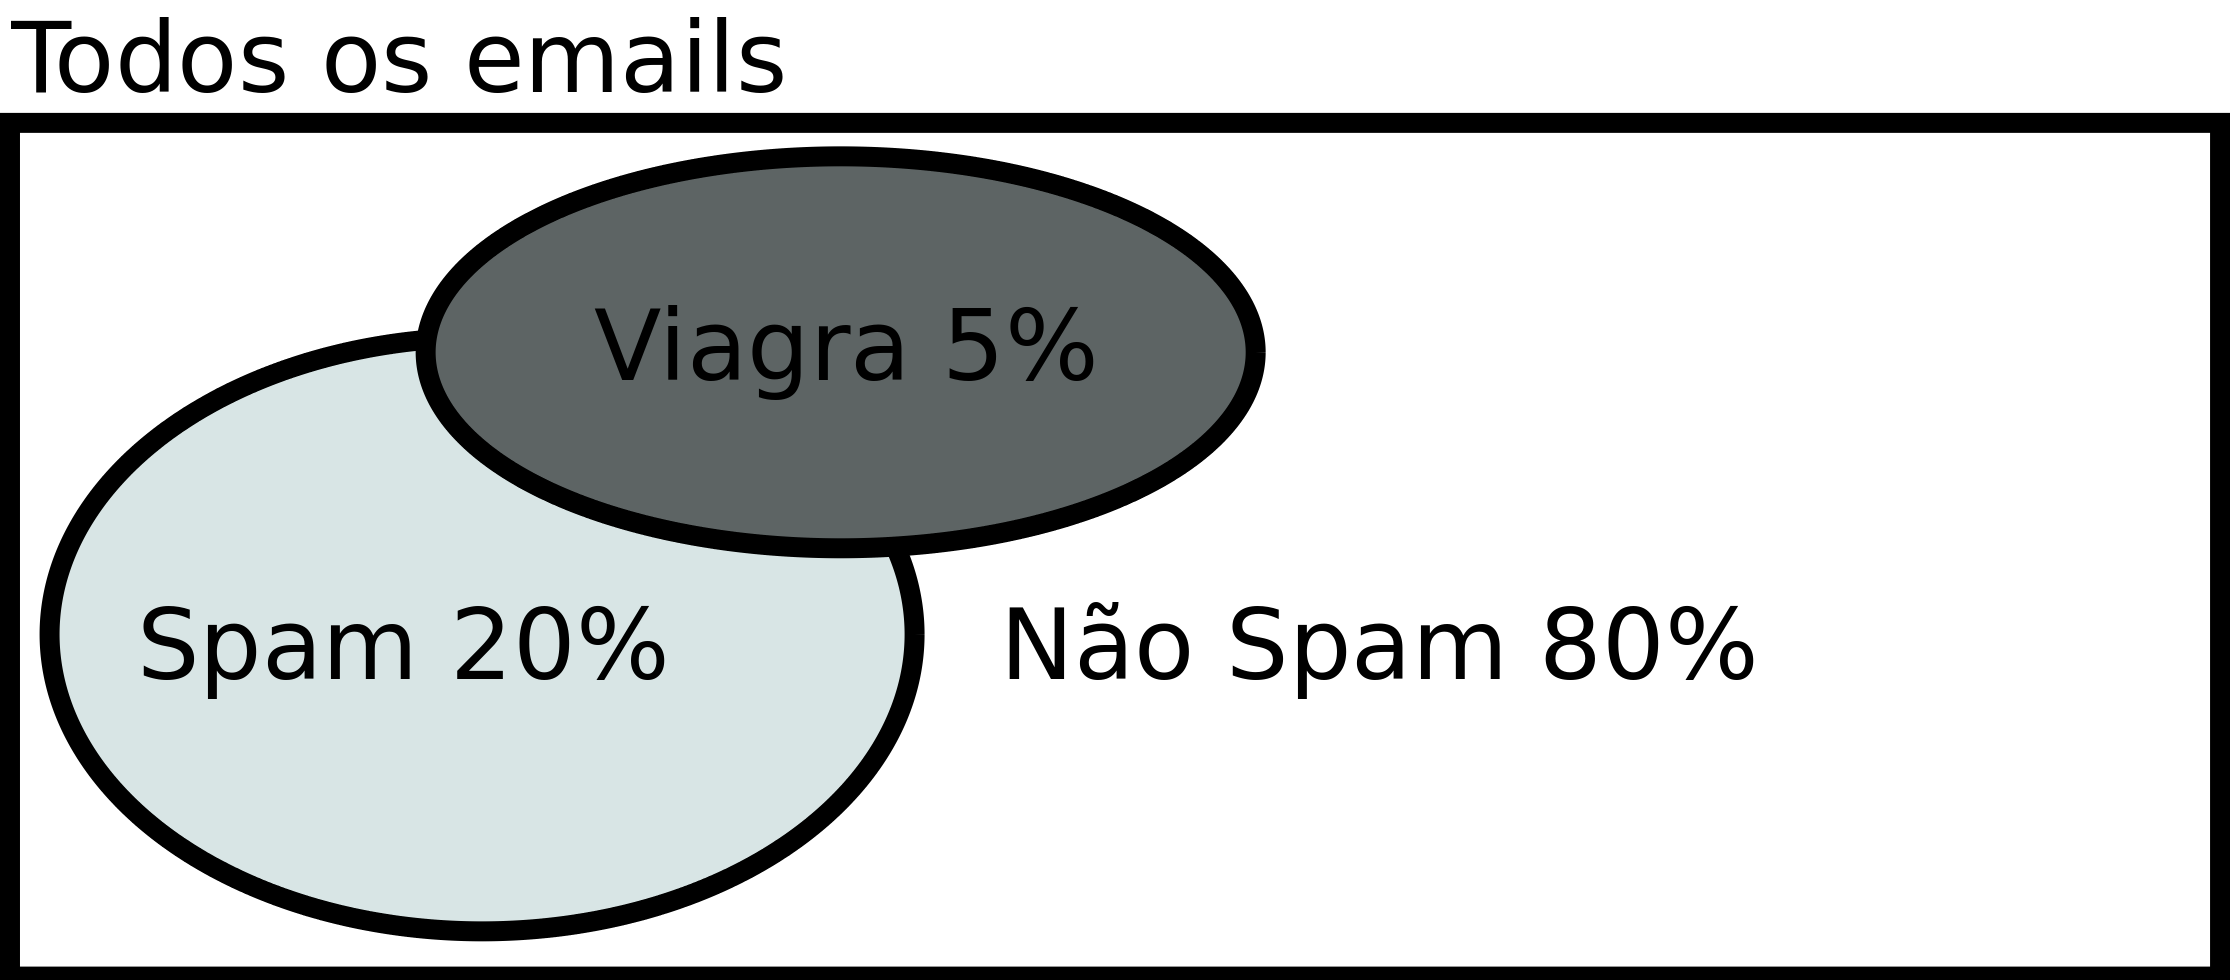
\includegraphics[width=7cm, height=4.5cm]{./secoes/conceitosFundamentais/pics/img/EventosNaoMutuamenteExclusivos.png}
	\label{FIGURA_EVENTOS_NAO_MUTUAMENTE_EXCLUSIVOS}
  \source{Adaptado de \citeonline{MachineLearningwithR2013}.}
\end{figure}
O evento viagra pode (ou não) ser um \emph{spam}, logo ele é conjunto mas nem todo o email com essa palavra é um \emph{spam}. É necessário calcular a probabilidade da intersecção dos eventos \emph{viagra} e \emph{spam} \(P(Spam \cap Viagra)\) que depende da probabilidade conjunta dos dois eventos (como a probabilidade de um evento está relacionada a outro).

Se todos os eventos forem independentes(não possuem relação [\(P(A \cap B) = P(A)P(B)\)]) é impossível prever um evento com dados de outro. No caso da não independência é válida a relação:
\begin{align}
P(A|B) =  \frac{P(B|A)P(A)}{P(B)} \Leftrightarrow \frac{P(A \cap B)}{P(B)} \label{BAYES}
\end{align}
Exemplificando para classificar um email como \emph{spam} ou \emph{não spam}, sem informações adicionais é possível alegar que há \(20\%\) de chance de ser um \emph{spam}, que é a probabilidade \emph{apriori}.

Agora suponha que você obteve mais informações e que a mensagem recebida contenha o termo \emph{Viagra}. A probabilidade desse termo ser utilizado em mensagens anteriores é chamado verossimilhança e a probabilidade do termo aparecer em qualquer mensagem é chamado verossimilhança marginal.

Aplicando o teorema de Bayes podemos calcular a probabilidade posteriori que metrifica a probabilidade de uma mensagem ser um \emph{spam}. Se a probabilidade for maior que \(50\%\) é mais parecido com spam.
\begin{align}
P(Spam|Viagra) =  \frac{\overbrace{P(Viagra|Spam)}^{\text{verossimilhança}} \overbrace{P(Spam)}^{\text{probabilidade apriori}}}{\underbrace{P(Viagra)}_{\text{verossimilhança marginal}}}
\end{align}
Para calcular esses componentes precisamos de uma tabela de frequência que armazena o número de ocorrências do termo \emph{Viagra} nos emails classificados como \emph{spam} e como \emph{não spam}(conjunto de treinamento), que será utilizada para construir uma tabela de verossimilhança.
\begin{table}[htbp]
	\centering
	\caption{Matriz de Frequência}
		\begin{tabular}{llll} \hline

		Frequência	& Contém Viagra	& Não Contém Viagra	& Total   \\ \hline
		Spam		& \(4\) 		& \(16\)			& \(20\)  \\ 
		Não Spam	& \(1\) 		& \(79\)			& \(80\)  \\ 
		Total		& \(5\) 		& \(95\)			& \(100\) \\ \hline
		
		\end{tabular}
	\label{tab:ExemploDeTabela1}
	\vspace{0.1cm}
  \source{Adaptado de \citeonline{MachineLearningwithR2013}.}
\end{table}
A Tabela \ref{tab:ExemploDeTabela1} permite construção da Tabela \ref{tab:ExemploDeTabela2} de verossimilhança dos dados de treinamento.
\bgroup
\def\arraystretch{1.5}
\begin{table}[htbp]
	\centering
	\caption{Matriz de Verossimilhança}
		\begin{tabular}{llll} \hline

		Frequência	& Contém Viagra		& Não Contém Viagra	& Total   \\ \hline
		Spam		& \(\frac{4}{20}\) 	& \(\frac{16}{20}\)	& \(20\)  \\ 
		Não Spam	& \(\frac{1}{80}\) 	& \(\frac{79}{80}\)	& \(80\)  \\ 
		Total		& \(\frac{5}{100}\) & \(\frac{95}{100}\)& \(100\) \\ \hline
		
		\end{tabular}
	\label{tab:ExemploDeTabela2}
	\vspace{0.1cm}
  \source{Adaptado de \citeonline{MachineLearningwithR2013}.}
\end{table}
\egroup
Utilizando a Tabela \ref{tab:ExemploDeTabela2} e a equação \eqref{BAYES} obtemos:
\begin{align}
\frac{P(Viagra|Spam)P(Spam)}{P(Viagra)} = \frac{\frac{4}{20} \frac{20}{100}}{\frac{1}{80}} = 3.2
\end{align}
que é uma probabilidade mais acurada que a baseada em independência.

\subsection{Rede Neural - classificador e regressor}
Redes neurais artificiais tem como inspiração o cérebro humano, seus neurônios e suas conexões. A computação tenta reproduzir este modelo de cérebro como uma relação de entradas e saídas ponderadas que são definidas por vários nós de processamento. Os quais são responsáveis por calcular a soma de entradas ponderadas e repassá-las para a função de ativação. Esta determina se um sinal será enviado (ou não) para o neurônio seguinte \cite{Haykin2007}.
\begin{figure}[H]
	\centering
 	\caption{Exemplo de neurônio.}
	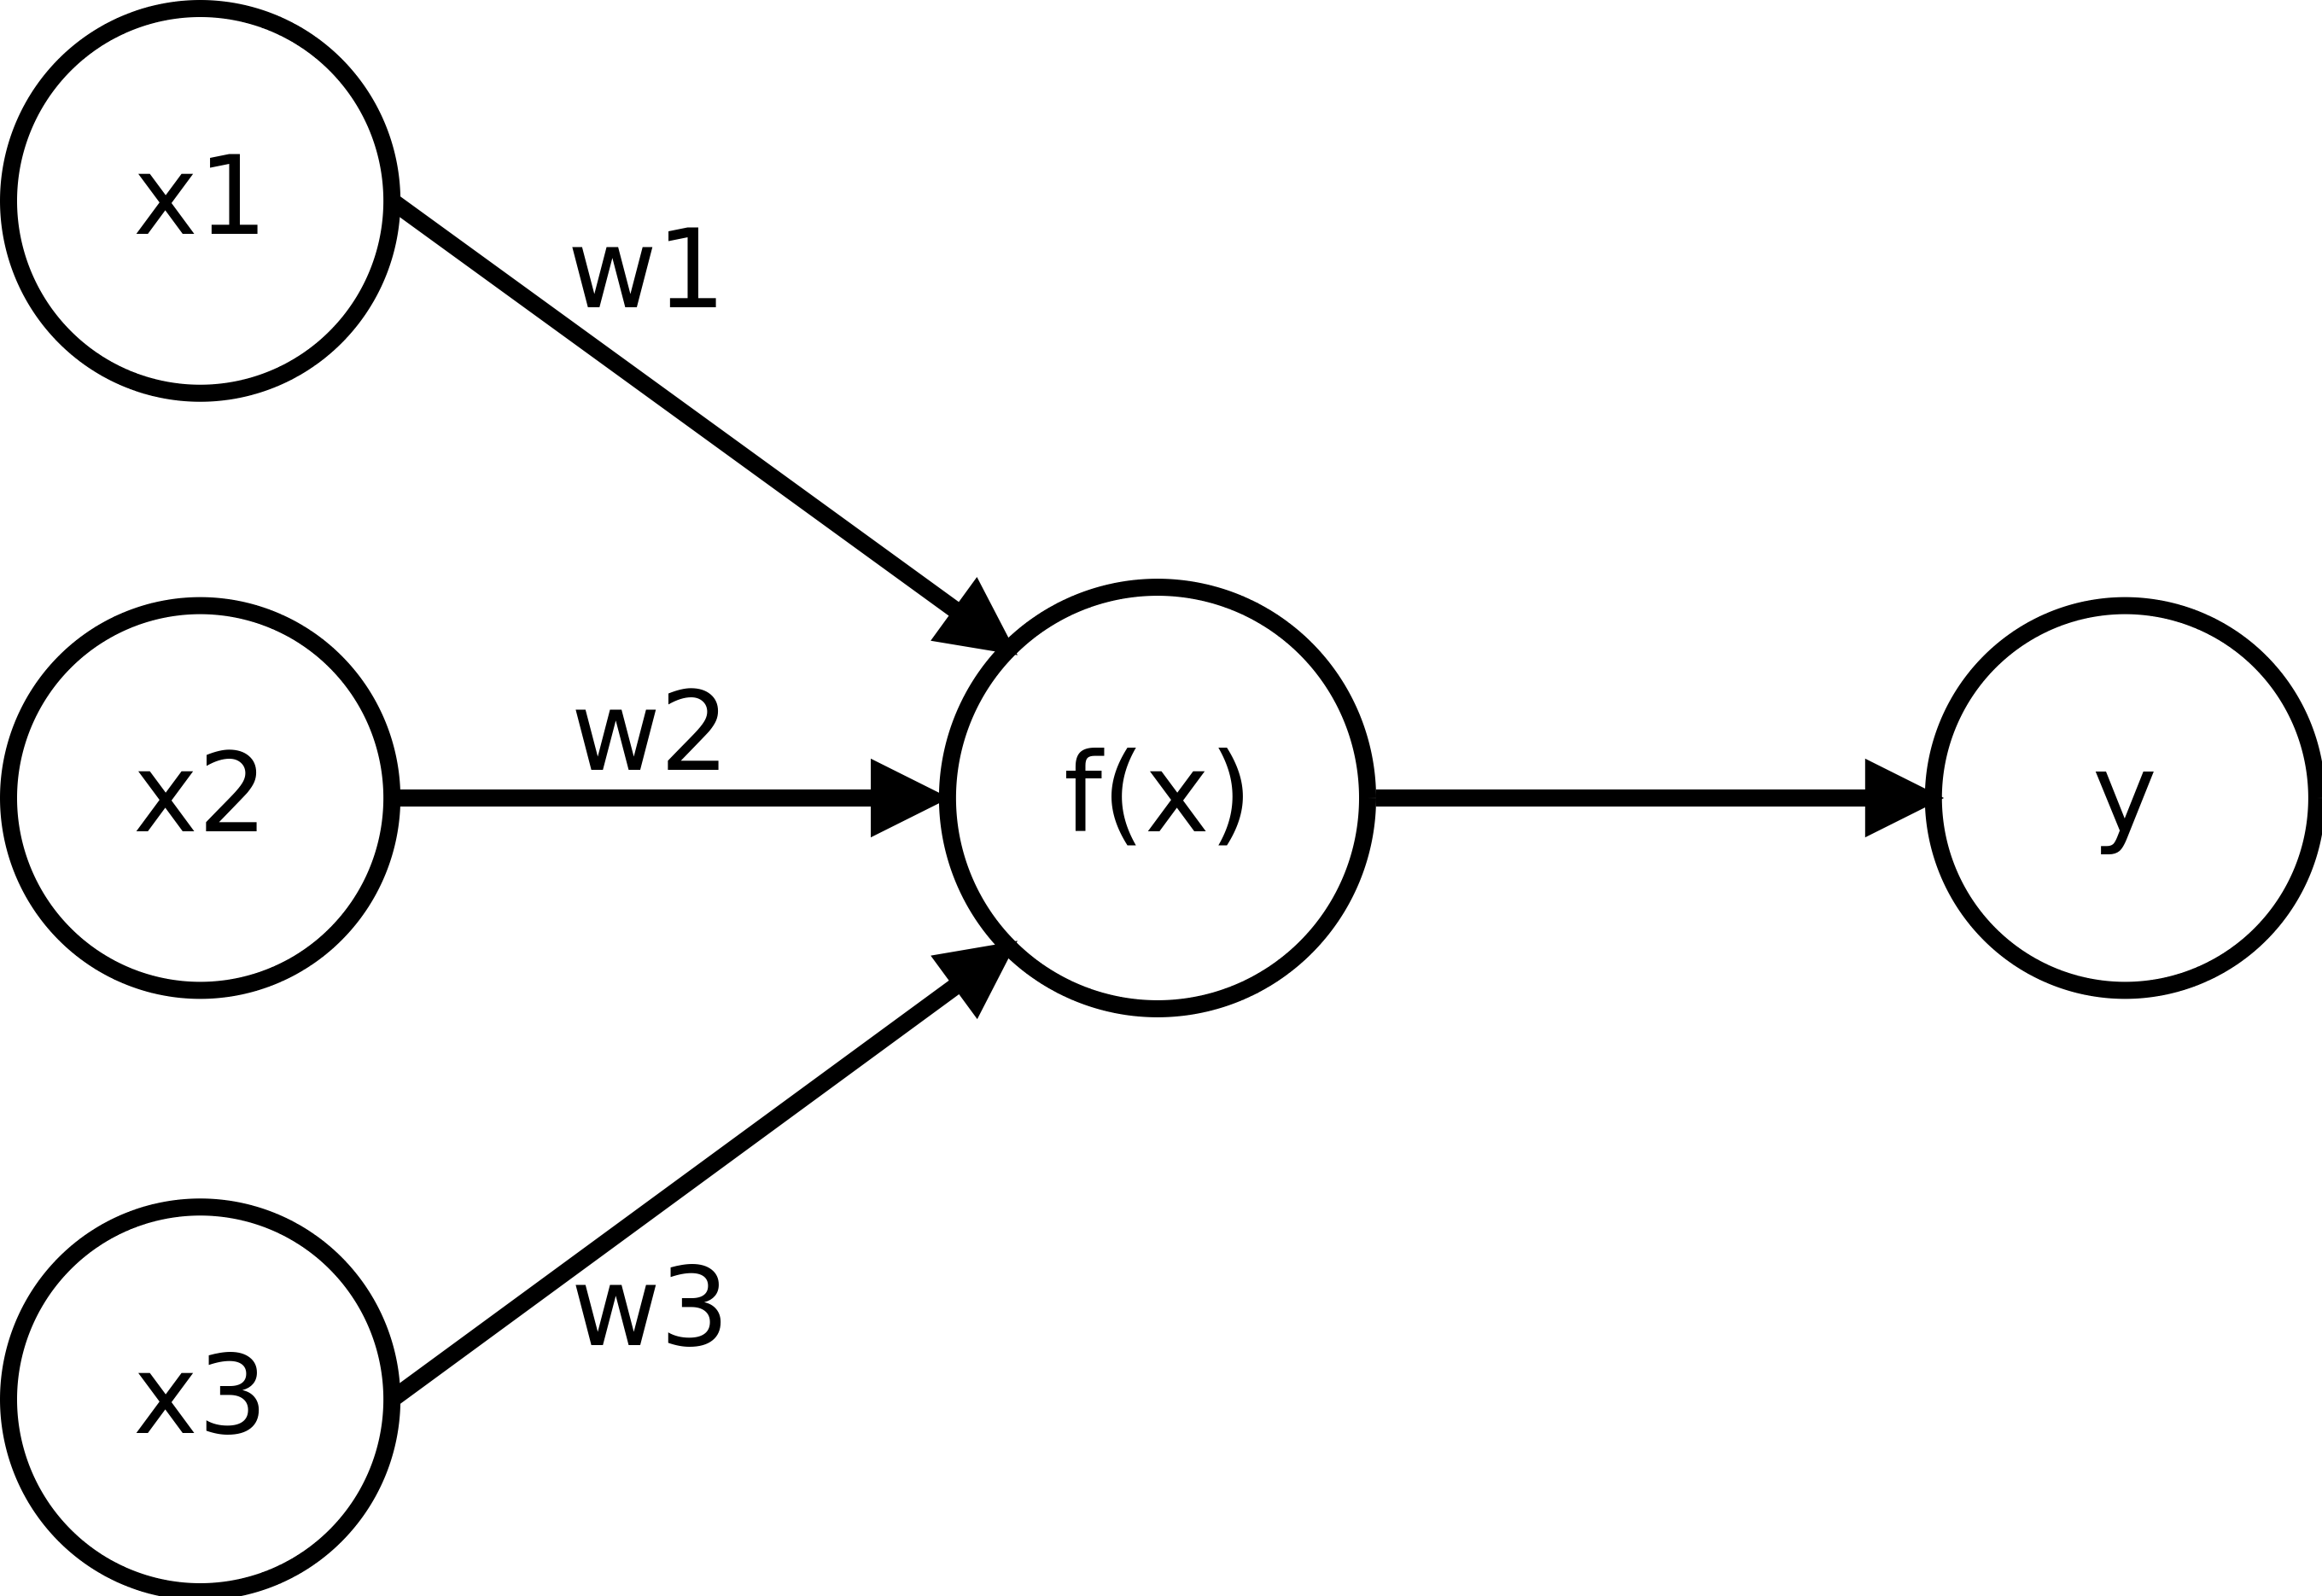
\includegraphics[width=5.5cm,height=3cm]{./secoes/conceitosFundamentais/pics/img/RedeNeural.png}
	\label{FIGURA_REDE_NEURAL_NEURONIO}
  \source{Adapatado de \citeonline{MachineLearningwithR2013}.}
\end{figure}
A Figura \ref{FIGURA_REDE_NEURAL_NEURONIO} apresenta um neurônio onde o vetor \(\mathbf{w}\), são os pesos sinápticos, o vetor \(\mathbf{x}\) são os \(n\) sinais de entrada, \(f(x)\) é a função de ativação e \(y\), é o sinal de saída que pode ser calculado por
\begin{align}
y(x) = f \left( \sum\limits_{i=1}^{n} w_{i}x_{i} \right)
\end{align}

Uma rede neural é um conjunto de neurônios conectados em uma determinada \emph{arquitetura}. A qual consiste no número de neurônios por camada, o tipo de conexão entre estes, o fluxo de informação entre neurônios, a função de ativação e o algoritmo de treinamento utilizado. No restante dessa seção serão detalhados os items da arquitetura citados.

Analisando a rede neural da Figura \ref{FIGURA_REDE_NEURAL_TOPOLOGIA} pode-se constatar que suas camadas são formadas por: i) três neurônios de entrada (representados pela letra \emph{x}), que recebem os dados diretamente da fonte; ii) dois neurônios ocultos (representados por \emph{h})), que recebem dados processados por neurônios e enviam estes dados para outros neurônios; e iii) um neurônio de saída (representado por \emph{y}) que apresenta a saída da rede.
\begin{figure}[H]
	\centering
 	  \caption{Topologia de rede neural.}
		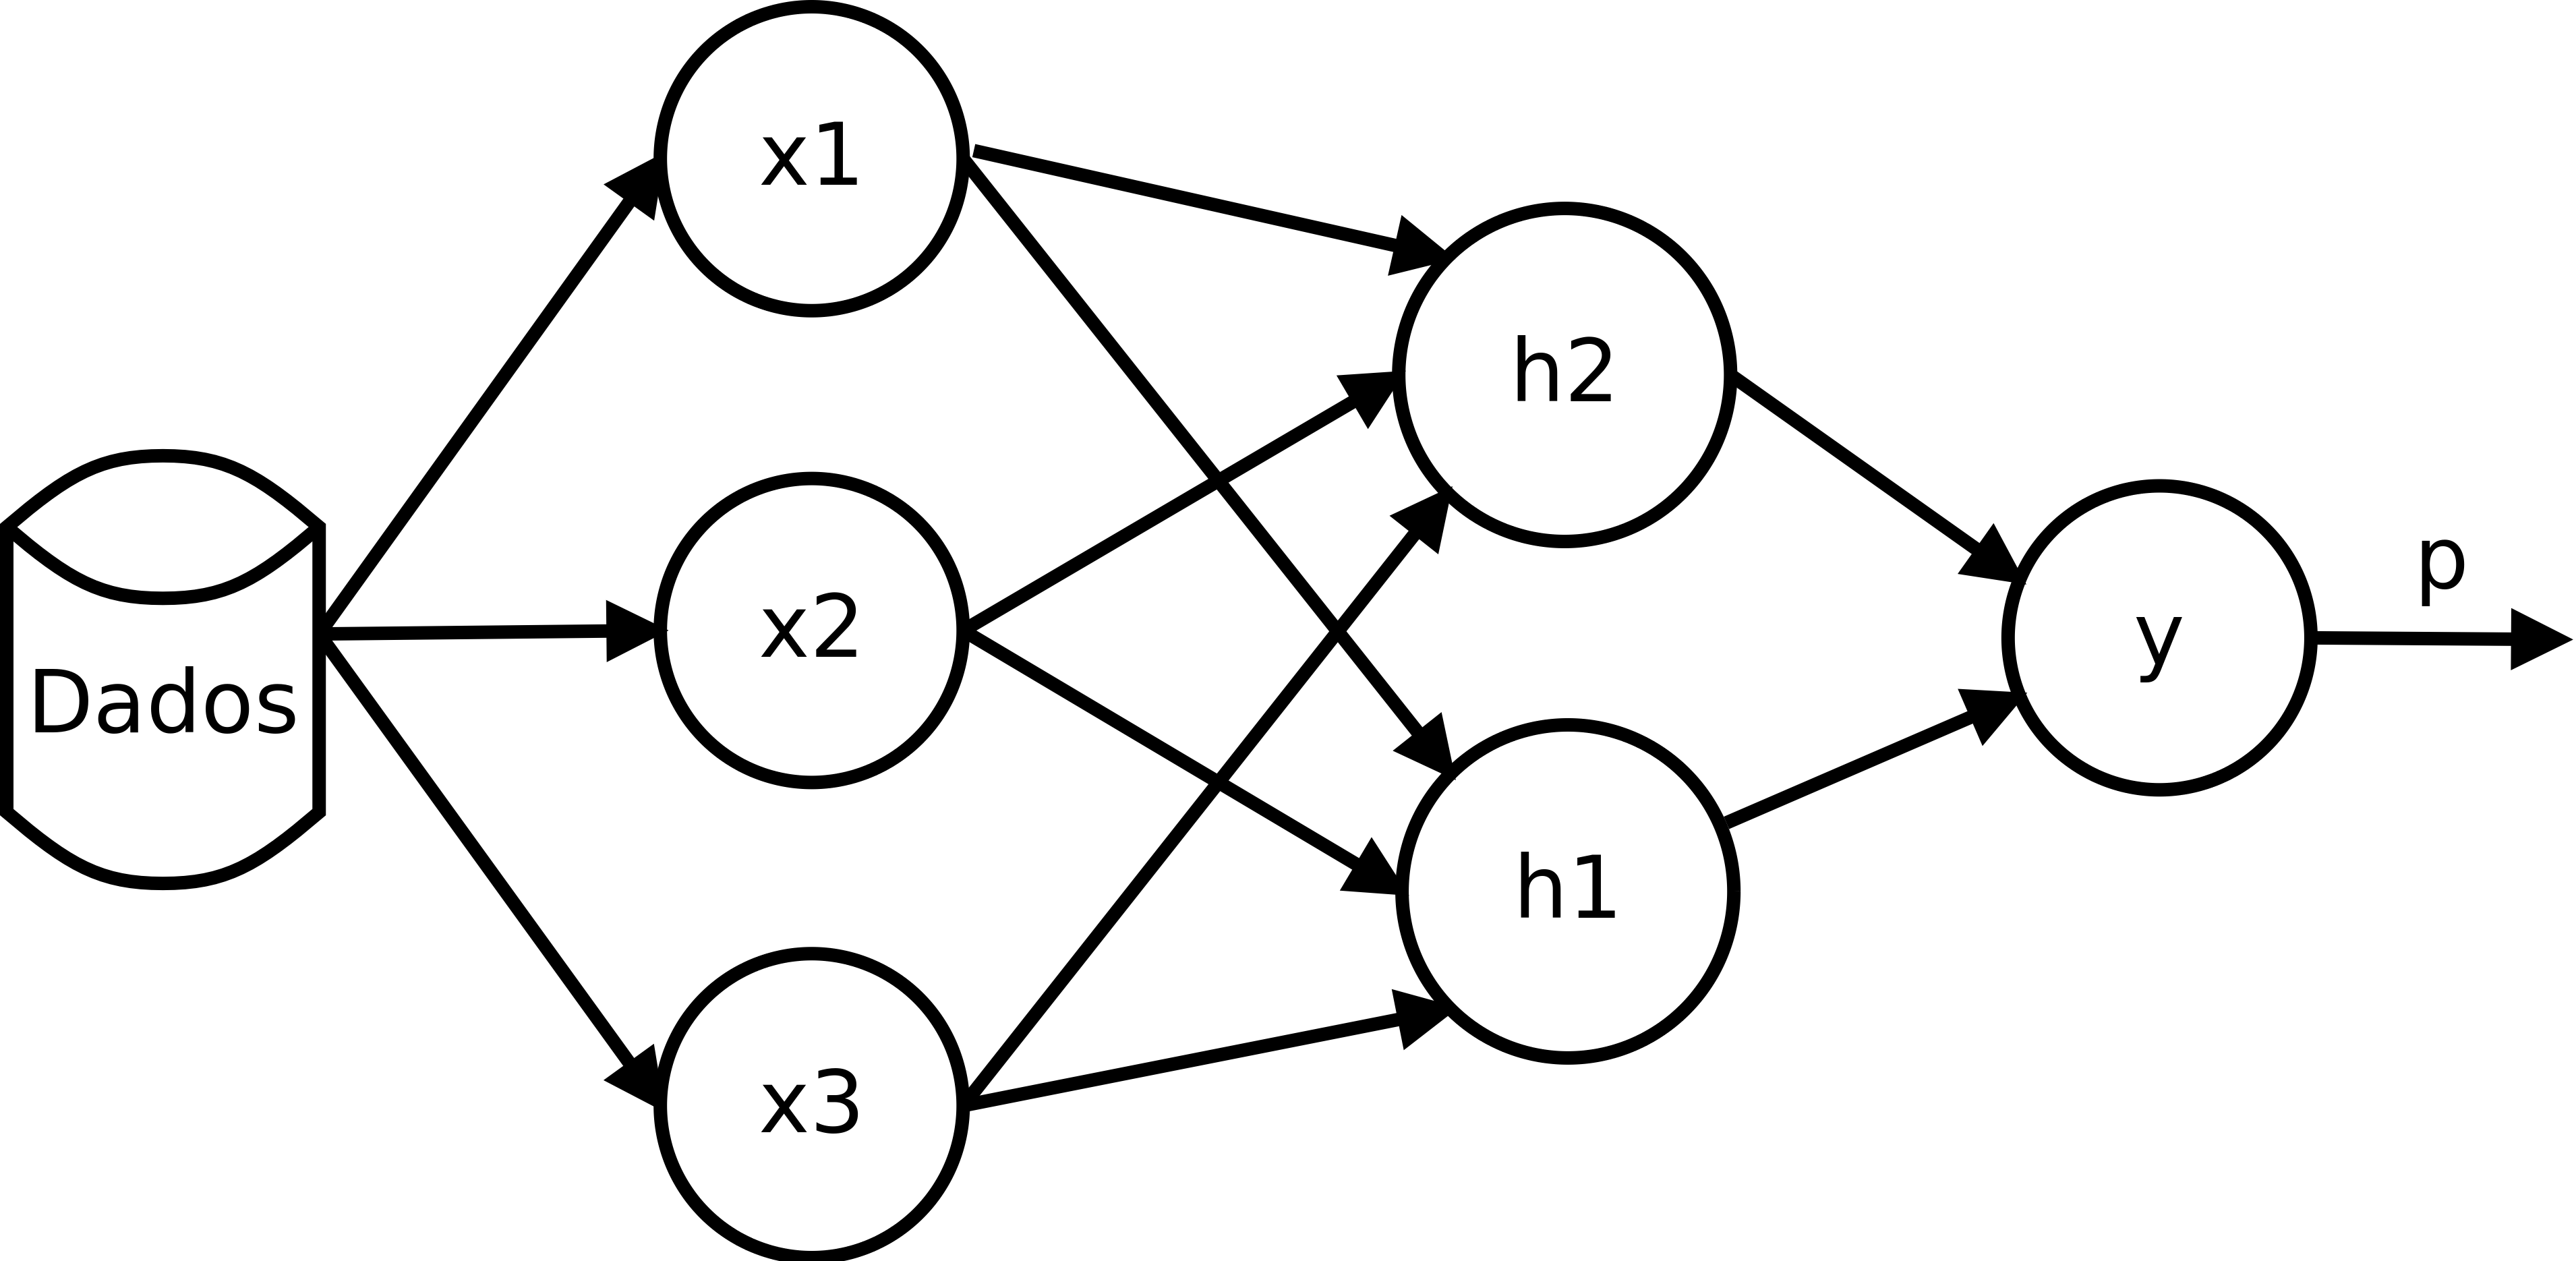
\includegraphics[width=8cm,height=5cm]{./secoes/conceitosFundamentais/pics/img/RedeNeuralTopologia.png}
	\label{FIGURA_REDE_NEURAL_TOPOLOGIA}
  \source{Adapatado de \citeonline{MachineLearningwithR2013}.}
\end{figure}
O tipo de conexão entre neurônios na Figura \ref{FIGURA_REDE_NEURAL_TOPOLOGIA} é denominado \emph{totalmente conectada}, onde todos os neurônios de uma camada estão conectados com todos os neurônios da camada seguinte. O fluxo de informação é denominado \emph{feedforward} pois os dados trafegam da direita para a esquerda sem retroalimentação, em outras palavras, no sentido das setas pretas.

A função de ativação \(f(x)\), exibida na Figura \ref{FIGURA_REDE_NEURAL_NEURONIO}, determina qual tipo de sinal será enviado para o neurônio seguinte. \citeonline{MachineLearningwithR2013} cita as seguintes funções de ativação, a função \emph{degrau} definida por
\begin{align}
f(x) = \begin{cases}
		0 \mbox{ se } x < 0 	 \\
		1 \mbox{ se } x \geq 0	 \label{EQU_FUNCAO_DEGRAU}				
	   \end{cases}
\end{align}
e a função \emph{sigmóide} definida por
\begin{align}
f(x) = \frac{1}{1 + e^{-x}} 	\label{EQU_FUNCAO_SIGMOIDE}
\end{align}

A escolha da função de ativação deve considerar possíveis restrições do algoritmo de treinamento, um exemplo de restrição do algoritmo \emph{backpropagation} é que a função deve ser diferenciável em todos os pontos. Apenas a função \emph{sigmóide} \eqref{EQU_FUNCAO_SIGMOIDE} apresenta esta propriedade.

O algoritmo de treinamento usado neste projeto, \emph{backpropagation}, possuí duas abordagens para treinar os dados: i) \emph{online}; e ii) \emph{batch}, neste projeto é usada a primeira forma. A qual atualiza os pesos sinápticos instância por instância iterativamente após serem apresentadas a rede neural \cite{Haykin2007}. Para explicar o funcionamento deste algoritmo é necessário compreender como calcular o erro de um neurônio \(j\) na iteração \(n\), como o da Figura \ref{FIGURA_REDE_NEURAL_NEURONIO_BACKPROPAGATION} que é calculado por
\begin{align}
e_{j}(n) = d_{j}(n) - y_{j}(n)	\label{EQU_REDE_NEURAL_ERRO_NEURONIO_J}
\end{align}
onde \(d_{j}(n)\) é o valor de saída esperado e \(y_{j}(n)\) é o valor de saída obtido. Além deste erro, é necessário calcular o valor de erro total da camada de saída que é calculado por
\begin{align}
\xi(n) = \frac{1}{2} \sum\limits_{j \in C} (e_{j})^{2}(n)	\label{EQU_REDE_NEURAL_ERRO_TODOS_OS_NEURONIOS_SAIDA}
\end{align}
onde \(C\) é o conjunto de neurônios na camada de saída da rede. O objetivo do treinamento é atualizar o vetor \(\mathbf{w}\) para minimizar \(\xi(n)\). Essa minimização é realizada pela técnica \emph{descida de gradiente} a qual começa calculando o vetor de gradiente de cada neurônio. Em seguida calcula o erro de cada neurônio para as duas possíveis situações: i) para os neurônios de saída (caso simples); e ii) para os neurônios de ocultos (caso complexo). Por fim, usa a regra delta para atualizar o valor \(\mathbf{w}\), esta regra tem como requisitos os cálculos: i) do vetor gradiente; e ii) o erro dos neurônios.
\begin{figure}[H]
	\centering
 	  \caption{Exemplo de neurônio de saída para cálculo do backpropagation.}
		\includegraphics[width=13cm,height=7cm]{./secoes/conceitosFundamentais/pics/img/NeuronioJ.png}
	\label{FIGURA_REDE_NEURAL_NEURONIO_BACKPROPAGATION}
  \source{\citeonline{Haykin2007}}
\end{figure}
A Figura \ref{FIGURA_REDE_NEURAL_NEURONIO_BACKPROPAGATION} exibe um neurônio \(j\) sendo alimentado por uma camada de neurônios à esquerda, denominada \(y_{i}\) onde \(i = 1, 2, 3 \ldots m\). Este neurônio tem o valor de entrada da função de ativação \(v_{j}(n)\), que é uma soma ponderada entre as entradas e seus pesos, calculada por
\begin{align}
v_{j}(n) = \sum\limits_{i = 0}^{m} w_{ji}(n)y_{i}(n)\label{EQU_REDE_NEURAL_SOMA_ATIVACAO_NEURONIO}
\end{align}
onde \(m\) é o número total de neurônios de entrada. O resultado da equação \eqref{EQU_REDE_NEURAL_SOMA_ATIVACAO_NEURONIO} é o parâmetro de entrada para a função de ativação, dessa forma é possível escrever
\begin{align}
y_{j}(n) = \varphi_{j}(v_{j}(n)) \label{EQU_REDE_NEURAL_SAIDA_NEURONIO}
\end{align}

A correção \(\Delta w_{ij}(n)\) aplicada nos pesos sinápticos \(w_{ij}(n)\) é proporcional a derivada parcial do erro total em relação aos pesos sinápticos \(\frac{\partial \xi(n)}{\partial w_{ji}(n)}\) e pode ser escrita, de acordo com a regra da cadeia, como
\begin{align}
\frac{\partial \xi(n)}{\partial w_{ji}(n)} =
\frac{\partial \xi(n)}{\partial e_{j}(n)} 		\,
\frac{\partial e_{j}(n)}{\partial y_{j}(n)} 	\,
\frac{\partial y_{j}(n)}{\partial v_{j}(n)} 	\,
\frac{\partial v_{j}(n)}{\partial w_{ji}(n)} \label{EQU_REDE_NEURAL_GRADIENTE}
\end{align}
onde a derivada parcial \(\frac{\partial \xi(n)}{\partial w_{ji}(n)}\) representa um fator de sensitividade que determina em qual direção no espaço de pesos devemos pesquisar pelas atualizações de \(w_{ji}(n)\). Cada uma das quatro derivadas parcias do lado direito da equação \eqref{EQU_REDE_NEURAL_GRADIENTE} será solucionada para encontrar o gradiente. Diferenciando os dois lados da equação \eqref{EQU_REDE_NEURAL_ERRO_TODOS_OS_NEURONIOS_SAIDA} em relação à \(e_{j}(n)\) é possível reescrevê-la como
\begin{align}
\frac{\partial \xi(n)}{\partial e_{j}(n)} = e_{j}(n) \label{EQU_REDE_NEURAL_DERIVADA_ERRO_TOTAL_SOBRE_ERRO}
\end{align}
diferenciando os dois lados da equação \eqref{EQU_REDE_NEURAL_ERRO_NEURONIO_J} em relação à \(y_{j}(n)\) é possível reescreve-la como
\begin{align}
\frac{\partial e_{j}(n)}{\partial y_{j}(n)} = -1 \label{EQU_REDE_NEURAL_DERIVADA_ERRO_NEURONIO_SOBRE_SINAL_SAIDA_NEURONIO}
\end{align}
diferenciando a equação \eqref{EQU_REDE_NEURAL_SAIDA_NEURONIO} em relação à \(v_{j}(n)\) é possível reescreve-la como
\begin{align}
\frac{\partial y_{j}(n)}{\partial v_{j}(n)} = \varphi^{'}(v_{j}(n)) \label{EQU_REDE_NEURAL_DERIVADA_SAIDA_NEURONIO_SOBRE_SOMA_ATIVACAO_NEURONIO}
\end{align}
diferenciando a equação \eqref{EQU_REDE_NEURAL_SOMA_ATIVACAO_NEURONIO} em relação à \(w_{ji}(n)\) é possível reescreve-la como
\begin{align}
\frac{\partial v_{j}(n)}{\partial w_{j}(n)} = y_{i}(n) \label{EQU_REDE_NEURAL_DERIVADA_SOMA_ATIVACAO_NEURONIO_SOBRE_PESOS}
\end{align}
substituindo as equações \eqref{EQU_REDE_NEURAL_DERIVADA_ERRO_TOTAL_SOBRE_ERRO}, \eqref{EQU_REDE_NEURAL_DERIVADA_ERRO_NEURONIO_SOBRE_SINAL_SAIDA_NEURONIO}, \eqref{EQU_REDE_NEURAL_DERIVADA_SAIDA_NEURONIO_SOBRE_SOMA_ATIVACAO_NEURONIO}, \eqref{EQU_REDE_NEURAL_DERIVADA_SOMA_ATIVACAO_NEURONIO_SOBRE_PESOS} na equação \eqref{EQU_REDE_NEURAL_GRADIENTE} pode-se reescrever o erro em função dos pesos da rede como
\begin{align}
\frac{\partial \xi(n)}{\partial w_{ji}(n)} =
-e_{j}(n)\varphi^{'}(v_{j}(n))y_{i}(n)
\label{EQU_REDE_NEURAL_GRADIENTE_VALORES_SUBSTITUIDOS}
\end{align}
a correção \(\Delta w_{ji}(n)\) que será aplicada nos pesos \(w_{ji}(n)\) é definida pela regra delta como
\begin{align}
\Delta w_{ji}(n) = - \eta \frac{\partial \xi(n)}{\partial w_{ji}(n)}
\label{EQU_REDE_NEURAL_ATUALIZACAO_PESOS}
\end{align}
onde \(\eta\) é a taxa de aprendizado. Substituindo a equação \eqref{EQU_REDE_NEURAL_GRADIENTE_VALORES_SUBSTITUIDOS} na equação \eqref{EQU_REDE_NEURAL_ATUALIZACAO_PESOS} define-se a regra delta como
\begin{align}
\Delta w_{ji}(n) = - \eta \delta_{j}(n)y_{i}(n)
\label{EQU_REDE_NEURAL_ATUALIZACAO_PESOS_COM_GRADIENTE_LOCAL}
\end{align}
onde o gradiente local \(\delta_{j}(n)\) é definido por
\begin{align}
\nonumber \delta_{j}(n) &= -\frac{\partial \xi(n)}{\partial v_{j}(n)} \\ 
 	      \delta_{j}(n) &= -\frac{\partial \xi(n)}{\partial e_{j}(n)} \, \frac{\partial e_{j}(n)}{\partial y_{j}(n)} \, \frac{\partial y_{j}(n)}{\partial v_{j}(n)}\label{EQU_REDE_NEURAL_GRADIENTE_LOCAL_ATUALIZACOES}\\
	      \delta_{j}(n) &= e_{j}(n)\varphi^{'}(v_{j}(n))
\label{EQU_REDE_NEURAL_GRADIENTE_LOCAL}
\end{align}

De acordo com a equação \eqref{EQU_REDE_NEURAL_GRADIENTE_LOCAL} o gradiente local \(\delta_{j}(n)\) para o neurônio de saída \(j\) é o produto do sinal de erro da saída \(e_{j}(n)\) para aquele neurônio e o derivativo \(\varphi^{'}(v_{j}(n))\) da função de ativação \cite{Haykin2007}.

A posição do neurônio na arquitetura da rede influência o calculo do gradiente local logo apresenta papel fundamental para o cálculo do erro. Se for um neurônio de saída pode-se utilizar a equação \eqref{EQU_REDE_NEURAL_ERRO_NEURONIO_J} para determinar \(e_{j}(n)\) que será utilizado para calcular o gradiente local com a equação \eqref{EQU_REDE_NEURAL_GRADIENTE_LOCAL}.
\begin{figure}[H]
	\centering
 	  \caption{Exemplo de neurônio oculto para cálculo do backpropagation.}
		\includegraphics[width=13cm,height=7cm]{./secoes/conceitosFundamentais/pics/img/NeuroniosJK.png}
	\label{FIGURA_REDE_NEURAL_NEURONIOS_BACKPROPAGATION}
  \source{\citeonline{Haykin2007}}
\end{figure}
Se o neurônio estiver localizado em uma camada oculta, não possuí erro associado diretamente, dessa forma é nescessário retropropagar o erro recursivamente pelos neurônios que estão conectados \cite{Haykin2007}. Um exemplo de neurônio oculto pode ser visto na arquitetura da Figura \ref{FIGURA_REDE_NEURAL_NEURONIOS_BACKPROPAGATION} onde o gradiente local do neurônio oculto \(j\), de acordo com a equação \eqref{EQU_REDE_NEURAL_GRADIENTE_LOCAL}, é dado por
\begin{align}
\delta_{j}(n) &= - \frac{\partial \xi(n)}{\partial y_{j}(n)} \, \frac{\partial y_{j}(n)}{\partial v_{j}(n)} \Leftrightarrow \label{EQU_REDE_NEURAL_GRADIENTE_LOCAL_CASO2}\\
\delta_{j}(n) &= - \frac{\partial \xi(n)}{\partial y_{j}(n)} \, \varphi^{'}(v_{j}(n))
\end{align}
o erro do neurônio \(j\), exibido pela Figura \ref{FIGURA_REDE_NEURAL_NEURONIOS_BACKPROPAGATION}, é dado por
\begin{align}
\xi(n) = \frac{1}{2} \sum\limits_{k \in C}(e_{k})^{2}(n) \label{EQU_REDE_NEURAL_ERRO_NEURONIO_OCULTO}
\end{align}
onde \(k\) é um neurônio de saída, diferenciando a equação \eqref{EQU_REDE_NEURAL_ERRO_NEURONIO_OCULTO} em relação à \(y_{j}(n)\) ten-se que
\begin{align}
\frac{\partial \xi(n)}{\partial y_{j}(n)} = \sum\limits_{k} \frac{\partial e_{k}(n)}{\partial y_{j}(n)}  \label{EQU_REDE_NEURAL_ERRO_NEURONIO_OCULTO_DERIVADA_SAIDA}
\end{align}
usando a regra da cadeia na equação \eqref{EQU_REDE_NEURAL_ERRO_NEURONIO_OCULTO_DERIVADA_SAIDA} pode-se escrevê-la como
\begin{align}
\frac{\partial \xi(n)}{\partial y_{j}(n)} = \sum\limits_{k} \frac{\partial e_{k}(n)}{\partial v_{k}(n)} \frac{\partial v_{k}(n)}{\partial y_{j}(n)} \label{EQU_REDE_NEURAL_ERRO_NEURONIO_OCULTO_DERIVADA_SAIDA_REGRA_CADEIA}
\end{align}
da Figura \ref{FIGURA_REDE_NEURAL_NEURONIOS_BACKPROPAGATION} percebe-se que o erro é dado por
\begin{align}
e_{k}(n) &= d_{k}(n) - y_{k}(n) \Leftrightarrow \\
e_{k}(n) &= d_{k}(n) - \varphi^{'}(v_{k}(n))
\end{align}
então é possível reescrever o derivativo da equação \eqref{EQU_REDE_NEURAL_ERRO_NEURONIO_OCULTO_DERIVADA_SAIDA_REGRA_CADEIA} como
\begin{align}
\frac{\partial e_{k}(n)}{\partial v_{k}(n)} &= -\varphi^{'}(v_{k}(n))	\label{EQU_REDE_NEURAL_DERIVATIVO_ERRO_SOBRE_SOMATORIO}	   
\end{align}
a soma ponderada do neurônio \(k\), proposto na Figura \ref{FIGURA_REDE_NEURAL_NEURONIOS_BACKPROPAGATION}, é dada por
\begin{align}
v_{k}(n) = \sum\limits_{j = 0}^{m} w_{kj}(n)y_{j}(n)  \label{EQU_REDE_NEURAL_SOMA_PESO_ENTRADA}
\end{align}
onde \(m\) é o número total de entradas (excluíndo bias) aplicados no neurônio \(k\), o peso sináptico \(w_{k0}\) é igual ao bias \(b_{k}(n)\) aplicado no neurônio \(k\). Diferenciando a equação \eqref{EQU_REDE_NEURAL_SOMA_PESO_ENTRADA} em relação a \(y_{j}(n)\) é obtido
\begin{align}
\frac{\partial v_{k}(n)}{\partial y_{j}(n)} = w_{kj}(n) \label{EQU_REDE_NEURAL_DERIVATIVO_SOMA_SOBRE_ERRO}
\end{align}
Utilizando as equações \eqref{EQU_REDE_NEURAL_DERIVATIVO_ERRO_SOBRE_SOMATORIO}, \eqref{EQU_REDE_NEURAL_SOMA_PESO_ENTRADA} e \eqref{EQU_REDE_NEURAL_DERIVATIVO_SOMA_SOBRE_ERRO} na equação \eqref{EQU_REDE_NEURAL_ERRO_NEURONIO_OCULTO_DERIVADA_SAIDA_REGRA_CADEIA} é obtido o derivativo desejado
\begin{align}
\frac{\partial \xi(n)}{\partial y_{j}(n)} &= \sum\limits_{k} e_{k}(n)\varphi{'}(v_{k}(n))w_{kj}(n) \\
\frac{\partial \xi(n)}{\partial y_{j}(n)} &= -\sum\limits_{k}\delta_{k}(n)w_{kj}(n) \label{EQU_REDE_NEURAL_ERRO_NEURONIO_SOBRE_SAIDA}
\end{align}
na segunda linha é utilizada a definição de gradiente local da equação \eqref{EQU_REDE_NEURAL_GRADIENTE_LOCAL_ATUALIZACOES} trocando o neurônio \(j\) por \(k\). Usando a equação \eqref{EQU_REDE_NEURAL_ERRO_NEURONIO_SOBRE_SAIDA} na equação \eqref{EQU_REDE_NEURAL_GRADIENTE_LOCAL_CASO2} obtem-se a fórmula do gradiente local como
\begin{align}
\delta_{j}(n) = \varphi^{'}(v_{j}(n)) \sum\limits_{k}\delta_{k}(n)w_{kj}(n)
\end{align}

O gradiente local \(\delta_{j}(n)\) exige o cálculo do erro de todos os neurônios da camada seguinte e os pesos sinápticos dessas conexões, dessa forma pode-se escrever a regra delta como
\begin{align}
\Delta w_{ji}(n) = \eta \delta_{j}(n)y_{j}(n)
\end{align}
que será usada para atualizar os pesos do vetor \(\mathbf{w}\) no decorrer do treinamento. A técnica de rede neural será usada como classificador e regressor nesse projeto. No primeiro caso são usadas as saídas da rede neural para atribuir classes as instâncias. No segundo caso são usados os pesos da rede neural treinada para predizer valores numéricos.

\subsection{SVM Binário}
Suport Vector Machines (SVM) é uma técnica que pode ser usada para classificar dados usando um hiperplano separador. O objetivo do SVM é escolher a posição do hiperplano tal que permita formar partições homogêneas de dados em ambos os lados da superfície de decisão. Considerando dados futuros a melhor escolha é aquela que maximize a margem entre os dados e o hiperplano separador, nesse caso, denominado \emph{hiperplano ótimo} \cite{MachineLearningwithR2013}. 

No decorrer dessa seção será detalhada a técnica de SVM inciando pelo caso de dados linearmente separáveis, seguida pelo uso das margens f\mbox{}lexíveis e finalizando com a generalização com uso do \emph{kernel trick}. As explicações desta seção são baseadas nas obras de \citeonline{Haykin2007}, \citeonline{LIMA2004}, \citeonline{Fletcher1987}, \citeonline{Stewart2013}, \citeonline{Burges1998}, \cite{Cristianini1999} e \citeonline{Chang2011}.

\noindent
Dado um conjunto de dados linearmente separáveis como
\begin{align}
(\{x_{1}, d_{1}\}), (\{x_{2}, d_{2}\}), \ldots (\{x_{N}, d_{N}\}) \text{ com } x \in R^{n} \text{ e } d_{i} \in \{+1, -1\}
\end{align}
onde o vetor \(\mathbf{x}\) representa os dados e o vetor \(\mathbf{d}\) representa as classes. Um hiperplano separador para estes dados é definido pela seguinte equação
\begin{align}
\mathbf{w^{T}}\mathbf{x} + b = 0 		\label{EQU_SVM_HIPERPLANO_DECISAO}
\end{align}
onde \(\mathbf{x}\) é o vetor de entradas, \(\mathbf{w^{T}} \) é um vetor de pesos transposto e \(b\) é um bias. Este hiperplano, para dados linearmente separáveis, acarreta nas seguintes restrições
\begin{align}
\mathbf{w}^{T}\mathbf{x} + b &\geq 0  	\qquad \textrm{ para } d_{i} = +1 \label{restricaoSVM01} \\
\mathbf{w}^{T}\mathbf{x} + b &< 0		\qquad \textrm{ para } d_{i} = -1 \label{restricaoSVM02}
\end{align}
dados um \(\mathbf{w}\) e um \(b\) o espaço que separa o hiperplano \eqref{EQU_SVM_HIPERPLANO_DECISAO} e os dados mais próximos é denominado margem de separação (\(\rho\)), a qual pode ser vista na Figura \ref{FIGURA_SVM_Vetores_Suporte}, o objetivo do SVM é maximizar esta margem. O hiperplano com margem máxima, conhecido por \emph{hiperplano ótimo} e contém os valores otimizados \(\mathbf{w_{0}}\) e \(b_{0}\), tem sua equação definida como
\begin{align}
\mathbf{w^{T}_{0}}\mathbf{x} + b_{0} = 0 								\label{EQU_SVM_HIPERPLANO_OTIMO}
\end{align}
o par de valores ótimos, \(\mathbf{w_{0}}\) e \(b_{0}\), devem satisfazer as seguintes restrições
\begin{align}
\mathbf{w}^{T}\mathbf{x} + b &\geq +1  	\qquad \textrm{ para } d_{i} = +1 \label{restricaoSVM010} \\
\mathbf{w}^{T}\mathbf{x} + b &< -1		\qquad \textrm{ para } d_{i} = -1 \label{restricaoSVM020}
\end{align}
para garantir que a solução seja única mesmo reescalando valores de \(\mathbf{w_{0}}\) e \(b_{0}\) pois a equação \eqref{EQU_SVM_HIPERPLANO_OTIMO} permanecerá inalterada \cite{LIMA2004}. Os pontos que satisfazem o sinal de igualdadedas condições \eqref{restricaoSVM010} e \eqref{restricaoSVM020} (que são os pontos mais próximos do hiperplano ótimo) são conhecidos por vetores de suporte, que são os pontos em azul na Figura \ref{FIGURA_SVM_Vetores_Suporte}. Com essas novas restrições é possível definir a função discriminante como
\begin{align}
g(x) = \mathbf{w^{T}_{0}}\mathbf{x} + b_{0} 							\label{EQU_SVM_FUNCAO_DISCRIMINANTE}
\end{align}
utilizando a função discriminante é possível definir a margem máxima como uma distância entre: i) hiperplano; e ii) ponto. Pois para um dado vetor de suporte \(\mathbf{x^{s}}\) para o qual \(d^{s} = +1\) ten-se que
\begin{align}
g(\mathbf{x^{s}}) = \mathbf{w^{T}_{0}}\mathbf{x} + b_{0} = \pm 1 \qquad \textrm{ para } d_{i} = \pm 1
\end{align}
dessa forma é possível escrever a distância entre os vetores de suporte e o hiperplano como
\begin{align}
r = \frac{g(\mathbf{x^{s}})}{||\mathbf{w_{0}}||} = 	\begin{cases} \label{equ_distancia_margem}
														\frac{1}{||\mathbf{w_{0}}||}  \textrm{ para } d^{s} = +1 \\
														\frac{-1}{||\mathbf{w_{0}}||} \textrm{ para } d^{s} = -1
													\end{cases}
\end{align}
usando a equação \eqref{equ_distancia_margem} é possível definir a margem ótima como a distância entre os vetores de suporte da classe \(1\) ao hiperplano ótimo acrescido da distância entre os vetores de suporte da classe \(2\) ao hiperplano ótimo obtendo
\begin{align}
\rho = 2r = \frac{2}{||\mathbf{w_{0}}||} \label{EQU_SVM_MARGEM_MINIMIZAR}
\end{align}
Portanto para encontrar a margem máxima, \(\rho\) na Figura \ref{FIGURA_SVM_Vetores_Suporte}, é necessário maximizar a norma Euclidiana do vetor de pesos definido pela equação \eqref{EQU_SVM_MARGEM_MINIMIZAR} ou de forma equivalente minimizar \(w\)
\begin{align}  
\Phi(w) = \frac{1}{2}\mathbf{w^{T}}\mathbf{w} \label{EQU_SVM_MARGEM_EQUIVALENTE_MAXIMIZAR}
\end{align}
que é um problema de otimização quadrática convexa e o fator \(\frac{1}{2}\) foi acrescentado para facilitar as derivações. Este tipo de problema pode ser solucionado em três etapas. A primeira é construir o lagrangiano, a segunda é derivar as condições de otimização e a terceira é solucionar o problema no espaço dual dos multiplicadores de Lagrange \cite{Haykin2007}.
\begin{figure}[H]
  \centering
  \caption{Vetores de suporte e margem do SVM.}
  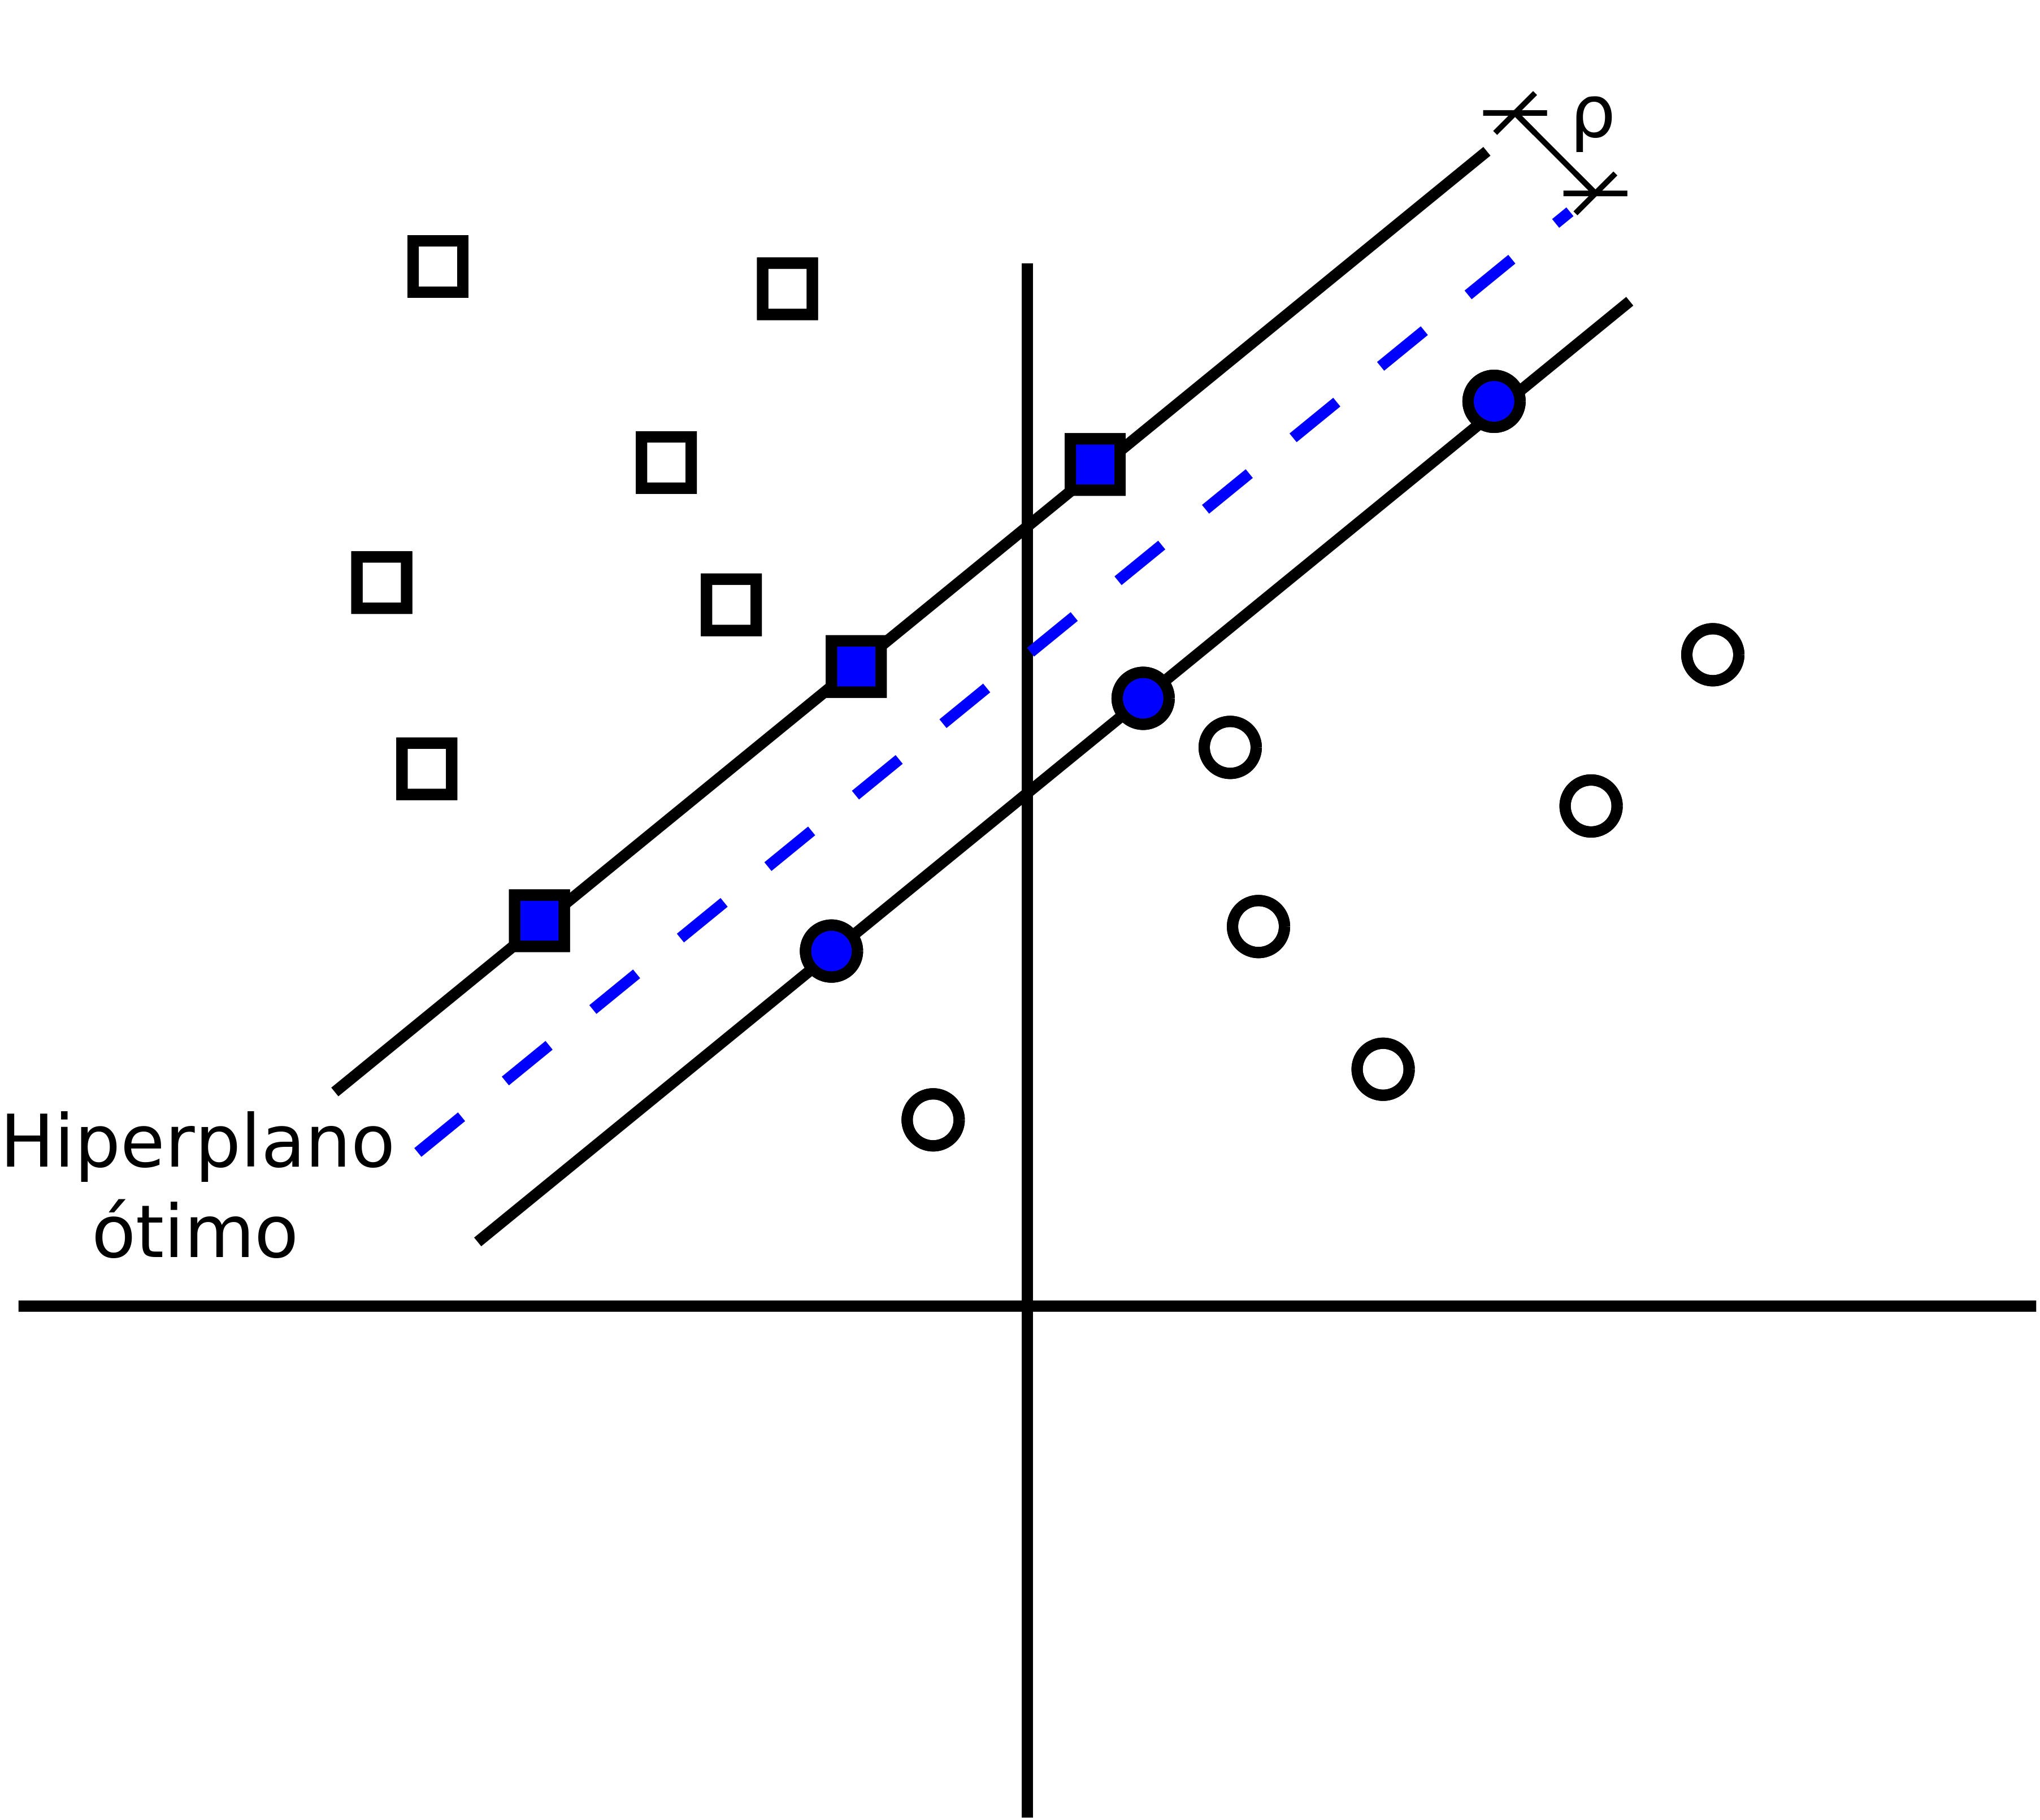
\includegraphics[width=8cm,height=6cm]{./secoes/conceitosFundamentais/pics/img/VetoresDeSuporteSVM.png}
  \label{FIGURA_SVM_Vetores_Suporte}
  \source{Adaptado de \citeonline{Haykin2007}.}
\end{figure}
\noindent
Para solucionar o problema de otimização quadrática definido pela equação \eqref{EQU_SVM_MARGEM_EQUIVALENTE_MAXIMIZAR} será utilizada a técnica de multiplicadores de Lagrange \cite{Stewart2013}. Para tal as restrições \eqref{restricaoSVM010} e \eqref{restricaoSVM020} foram combinadas em apenas uma restrição equivalente
\begin{align}
d_{i}(\mathbf{w^{T}}\mathbf{x} + b )  \geq 1  \qquad \textrm{ para } i = 1, 2, 3, \ldots, N \label{EQU_SVM_RESTRICAO_CONJUNTA}
\end{align}
o que permite escrever o seguinte Lagrangiano
\begin{align}
J(\mathbf{w}, b, \alpha) = \frac{1}{2}\mathbf{w^{T}}\mathbf{w} - \sum\limits_{i=1}^{N} \alpha_{i}[d_{i}(\mathbf{w^{T}}\mathbf{x} + b) - 1] \label{EQU_SVM_LAGRANGIANO_PRIMAL}
\end{align}
onde o primeiro termo é a função a ser minimizada e o segundo é a restrição reforçada pelos multiplicadores de Lagrange \(\mathbf{\alpha}\). A solução da equação \eqref{EQU_SVM_LAGRANGIANO_PRIMAL} é dada pelo ponto de sela do Lagrangiano que deve ser minimizado em relação a \(\mathbf{w}\) e \(b\), isto requer duas condições
\begin{align}
 \frac{\partial J(\mathbf{w}, b, \alpha)}{\partial \mathbf{w}} = 0	\label{EQU_SVM_PONTO_SELA_W}\\
 \frac{\partial J(\mathbf{w}, b, \alpha)}{\partial b} = 0  	\label{EQU_SVM_PONTO_SELA_B}
\end{align}
aplicando a condição \eqref{EQU_SVM_PONTO_SELA_W} na equação \eqref{EQU_SVM_LAGRANGIANO_PRIMAL} obten-se 
\begin{align}
\mathbf{w} = \sum\limits_{i=1}^{N} \alpha_{i}d_{i}\mathbf{x_{i}}  \label{EQU_SVM_PONTO_SELA_W_RESTRICAO_OBTIDA}
\end{align}
aplicando a condição \eqref{EQU_SVM_PONTO_SELA_B} na equação \eqref{EQU_SVM_LAGRANGIANO_PRIMAL} obten-se 
\begin{align}
\sum\limits_{i=1}^{N} \alpha_{i}d_{i} = 0 \label{EQU_SVM_PONTO_SELA_B_RESTRICAO_OBTIDA}
\end{align}
a solução do vetor \(\mathbf{w}\) é dada pelo conjunto de treinamento e é única, porém essa afirmação é falsa para os multiplicadores de Lagrange \(\alpha_{i}\). Para evitar isso é possível modelar a forma dual do problema que apresenta como vantagem a solução ser dada pelos próprios mulplicadores de Lagrange.

Segundo \citeonline{Fletcher1987} o problema dual pode ser formulado com duas premissas. A primeira, é que se o problema primal tem uma solução ótima o dual também possuí com os mesmos valores de ótimo e se \(\mathbf{w_{0}}\) é a solução ótima para o problema primal, \(\alpha_{0}\) é a solução ótima para o problema dual é suficiente e necessário que \(\mathbf{w_{0}}\) seja factível para o problema primal e
\begin{align}
J(\mathbf{w_{0}}, b_{0}, \alpha_{0}) = \min_{\mathbf{w}} J(\mathbf{w}, b, \alpha)
\end{align}
Dessa forma é possível formular o problema dual expandindo a equação \eqref{EQU_SVM_LAGRANGIANO_PRIMAL} para
\begin{align}
J(\mathbf{w}, b, \alpha) = \frac{1}{2}\mathbf{w^{T}}\mathbf{w} + \sum\limits_{i=1}^{N} \alpha_{i}d_{i}\mathbf{w^{T}}\mathbf{x_{i}} - b\sum\limits_{i=1}^{N} \alpha_{i}d_{i} + \sum\limits_{i=1}^{N} \alpha_{i} \label{EQU_SVM_LAGRANGIANO_PRIMAL_EXPANDIDO}
\end{align}
o terceiro termo da equação \eqref{EQU_SVM_LAGRANGIANO_PRIMAL_EXPANDIDO} é zero segundo a restrição \eqref{EQU_SVM_PONTO_SELA_B_RESTRICAO_OBTIDA} podendo ser removido, pela restrição \eqref{EQU_SVM_PONTO_SELA_W_RESTRICAO_OBTIDA} é possível escrever
\begin{align}
\mathbf{w^{T}} &= \sum\limits_{i=1}^{N} \alpha_{i}d_{i}\mathbf{w^{T}}\mathbf{x_{i}} \\
\mathbf{w^{T}}\mathbf{w} &= \sum\limits_{i=1}^{N} \sum\limits_{j=1}^{N} \alpha_{i}\alpha_{j}d_{i}d_{j}\mathbf{x_{i}^{T}}\mathbf{x_{j}} \label{EQU_SVM_LAGRANGIANO_TROCA1}
\end{align}
agora é possível reformular a função \(J(\mathbf{w}, b, \alpha) = Q(\alpha)\) e usando o valor de \eqref{EQU_SVM_LAGRANGIANO_TROCA1} é possível escrever o problema dual como
\begin{align}
Q(\alpha) = \sum\limits_{i=1}^{N} \alpha_{i} - \frac{1}{2} \sum\limits_{i=1}^{N} \sum\limits_{j=1}^{N} \alpha_{i}\alpha_{j}d_{i}d_{j}\mathbf{x_{i}^{T}}\mathbf{x_{j}} \label{EQU_SVM_LAGRANGIANO_DUAL}
\end{align}
dessa forma é possível reformular o problema de otimização quadrática para maximizar a função objetivo como
\begin{align}
Q(\alpha) = \sum\limits_{i=1}^{N} \alpha_{i} - \frac{1}{2} \sum\limits_{i=1}^{N} \sum\limits_{j=1}^{N} \alpha_{i}\alpha_{j}d_{i}d_{j}\mathbf{x_{i}^{T}}\mathbf{x_{j}} \label{EQU_SVM_OBJETIVO_DUAL}
\end{align}
com as restrições
\begin{align}
\sum\limits_{i=1}^{N} \alpha_{i}d_{i} &= 0 \\
\alpha_{i} &\geq 0	\qquad \textrm{ para } i = 1,2,3,\ldots, N
\end{align}
a nova função objetivo tem como vantagem depender exclusivamente dos dados de treinamento em forma de produto vetorial. Os valores ótimos de \(\alpha\) denominados \(\alpha_{0}\) são aqueles iguais a zero para os vetores de suporte e os diferentes de zero para os outros dados de treinamento. Determinar o vetor de peso ótimo (\(\mathbf{w_{0}}\)) pode ser feito usando a equação \eqref{EQU_SVM_PONTO_SELA_W_RESTRICAO_OBTIDA} tal que
\begin{align}
\mathbf{w_{0}} = \sum\limits_{i=1}^{N_{S}} \alpha_{0,i}d_{i}\mathbf{x_{i}} \label{EQU_SVM_W_OTIMO}
\end{align}
onde \(N_{S}\) são os vetores de suporte onde os valores de \(\alpha\) são diferentes de zero. Para o cálculo do bias ótimo (\(b_{0}\)) pode-se utilizar \(\mathbf{w_{0}}\) e 
\begin{align}
g(\mathbf{x^{s}}) = \mathbf{w_{0}^{T}}\mathbf{x^{s}} + b_{0} = \pm 1
\end{align}
pode-se escrever
\begin{align}
b_{0} &= 1 - \mathbf{w_{0}^{T}}\mathbf{x^{s}} \Leftrightarrow \\
b_{0} &= 1 - \sum\limits_{i=1}^{N_{S}} \alpha_{0,i}d_{i}\mathbf{x_{i}^{T}}\mathbf{x^{s}}
\end{align}
onde \(\mathbf{x^{s}}\) é um vetor de suporte cujo multiplicador de Lagrange é diferente de zero. 

%Nao separavel
O caso onde os dados \textbf{não são linearmente separáveis} pode ser visualizado na Figura \ref{FIGURA_SVM_Caso_Nao_Separavel} em dois casos possíveis. A parte \textbf{a} exibe o caso onde o dado foi classificado corretamente, do lado correto do hiperplano ótimo, porém após os vetores de suporte. Enquanto que a parte \textbf{b} exibe um erro de classificação pois o dado da classe \emph{círculo}, em vermelho, está localizada após o hiperplano ótimo. Nessas situações uma possível solução é tentar minimizar o erro de classificação usando variáveis de \emph{folga} (\(\xi_{i}\)), para tal a equação \eqref{EQU_SVM_RESTRICAO_CONJUNTA} é atualizada para 
\begin{align}
d_{i}(\mathbf{w^{T}}\mathbf{x} + b )  \geq 1 - \xi_{i} \qquad \textrm{ para } i = 1, 2, 3, \ldots, N
\end{align}
as variáveis \(\xi_{i}\) metrificam o desvio de um ponto ao hiperplano ótimo. Dessa forma para valores \(0 < \xi_{i} \leq 1\) significa que o dado se encontra no lado correto da superfície de decisão, para valores \(\xi_{i} > 1\) o dado está do lado errado da superfície de decisão. Portanto o objetivo, dessa formulação de SVM (que considerando dados não separáveis), é minimizar a função
\begin{align}
\Phi(\xi) &= \sum\limits_{i=1}^{N}I(\xi -1) \label{EQU_MINIMIZAR_MARGEM_SUAVE}\\
I(\xi) 	  &= \begin{cases}
				0 \textrm{ se } \xi \leq 0 \\
				1 \textrm{ se } \xi > 0 
			 \end{cases} 
\end{align}
minimizar a equação \eqref{EQU_MINIMIZAR_MARGEM_SUAVE} é um problema NP completo, para tornar este problema tratável será usada a seguinte aproximação da equação \eqref{EQU_MINIMIZAR_MARGEM_SUAVE}
\begin{align}
\Phi(\xi) &= \sum\limits_{i=1}^{N} \xi \label{EQU_MINIMIZAR_MARGEM_SUAVE_APROX}
\end{align}
dessa forma é possível reescrever a equação \eqref{EQU_MINIMIZAR_MARGEM_SUAVE_APROX} em função do vetor de pesos \(\mathbf{w}\) como
\begin{align}
\Phi(\mathbf{w}, \xi) &= \frac{1}{2}\mathbf{w^{T}}\mathbf{w} + C\sum\limits_{i=1}^{N} \xi \label{EQU_MINIMIZAR_MARGEM_SUAVE_APROX_SVM}
\end{align}

Onde primeiro termo (em relação ao sinal de igualdade) é relacionado ao problema de minimizar a norma euclidiana do vetor de pesos, existente pela definição do SVM. O segundo termo controla o problema de dados não separáveis, o qual funciona como um teto do número de erros aceitos no processo de treinamento. Quanto maior o valor da variável \(C\) maior o número de pontos fora da curva no conjunto de dados, quanto menor seu valor espera-se um conjunto de dados com menos \emph{outliers}.
\begin{figure}[H]
  \centering
  \caption{SVM com dados não linearmente separáveis.}
  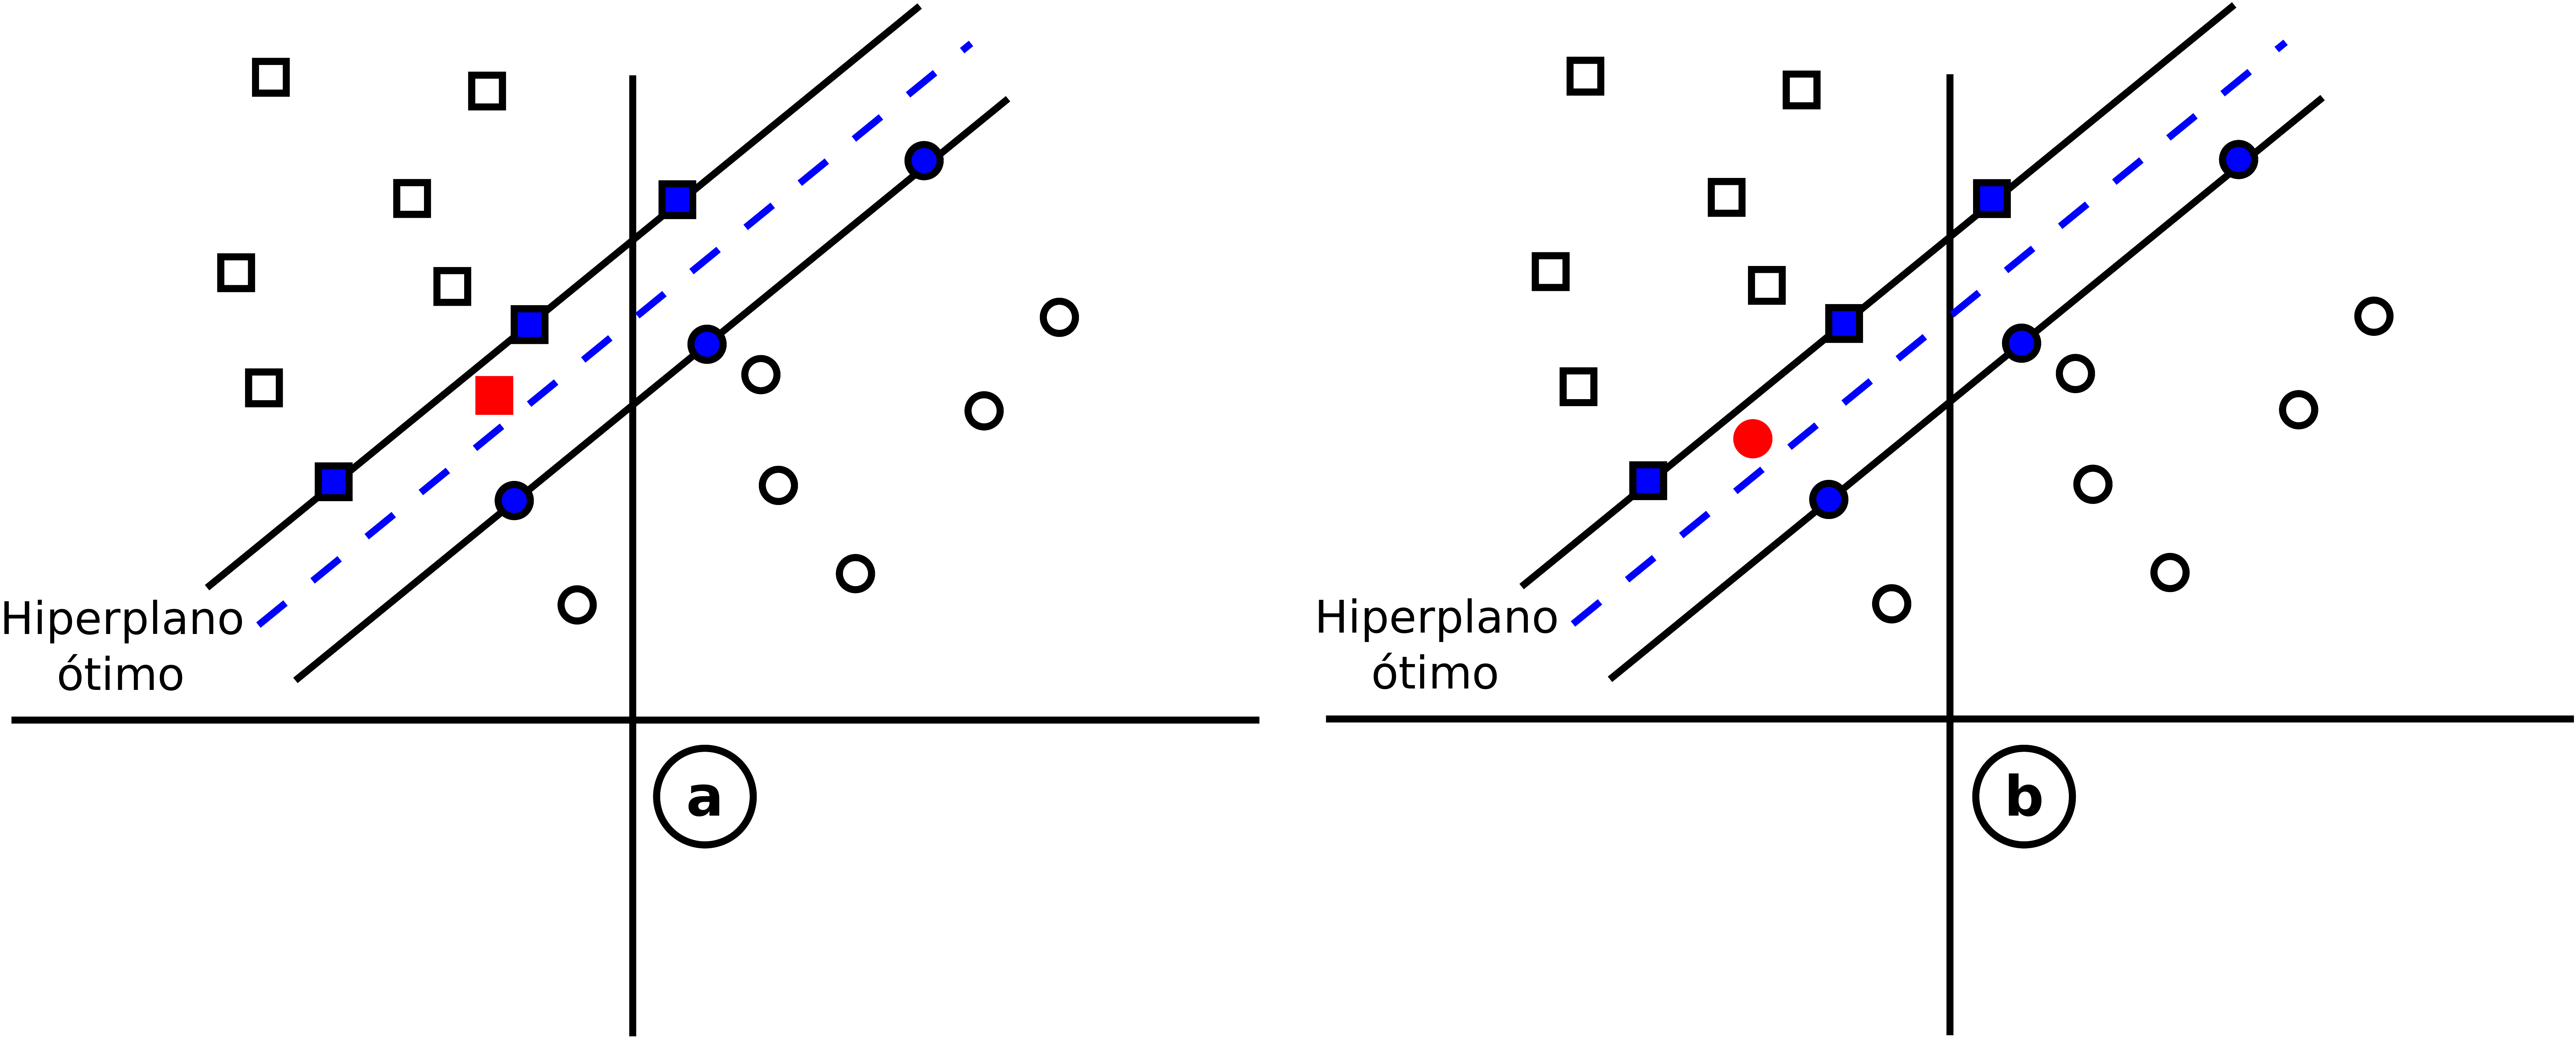
\includegraphics[width=14cm,height=7cm]{./secoes/conceitosFundamentais/pics/img/VetoresDeSuporteSVM_casoNaoSeparavel.png}
  \label{FIGURA_SVM_Caso_Nao_Separavel}
  \source{Adapatado de \citeonline{Haykin2007}.}
\end{figure}
Dessa forma, o problema pode ser visto como um caso especial do caso linearmente separável. Permitindo reformular o primal anterior ( ver equação \eqref{EQU_SVM_LAGRANGIANO_PRIMAL}) como
\begin{align}
J(\mathbf{w}, b, \alpha) = \frac{1}{2}\mathbf{w^{T}}\mathbf{w} + C\sum\limits_{i=1}^{N}\xi_{i} + \sum\limits_{i=1}^{N} \alpha_{i}[d_{i}(\mathbf{w^{T}}\mathbf{x} + b) - 1] - \sum\limits_{i=1}^{N}\beta \xi_{i}  \label{EQU_SVM_LAGRANGIANO_PRIMAL_NAO_SEPARAVEL}
\end{align}
cujo ponto de mínimo é dado pelas condições
\begin{align}
 \frac{\partial J(\mathbf{w}, b, \alpha)}{\partial \mathbf{w}} = 0	\label{EQU_SVM_PONTO_SELA_W_NAO_SEPARAVEL}\\
 \frac{\partial J(\mathbf{w}, b, \alpha)}{\partial b} = 0  			\label{EQU_SVM_PONTO_SELA_B_NAO_SEPARAVEL}\\
 \frac{\partial J(\mathbf{w}, b, \alpha)}{\partial \xi} = 0  		\label{EQU_SVM_PONTO_SELA_xi_NAO_SEPARAVEL}
\end{align}
aplicando a condição \eqref{EQU_SVM_PONTO_SELA_W_NAO_SEPARAVEL} na equação \eqref{EQU_SVM_LAGRANGIANO_PRIMAL_NAO_SEPARAVEL} obten-se 
\begin{align}
w = \sum\limits_{i=1}^{N} \alpha_{i}d_{i}x_{i}  \label{EQU_SVM_PONTO_SELA_W_RESTRICAO_OBTIDA_NAO_SEPARAVEL}
\end{align}
aplicando a condição \eqref{EQU_SVM_PONTO_SELA_B_NAO_SEPARAVEL} na equação \eqref{EQU_SVM_LAGRANGIANO_PRIMAL_NAO_SEPARAVEL} obten-se 
\begin{align}
\sum\limits_{i=1}^{N} \alpha_{i}d_{i} = 0 \label{EQU_SVM_PONTO_SELA_B_RESTRICAO_OBTIDA_NAO_SEPARAVEL}
\end{align}
aplicando a condição \eqref{EQU_SVM_PONTO_SELA_xi_NAO_SEPARAVEL} na equação \eqref{EQU_SVM_LAGRANGIANO_PRIMAL_NAO_SEPARAVEL} obten-se
\begin{align}
\alpha_{i}+\beta_{i} = C \label{EQU_SVM_PONTO_SELA_xi_RESTRICAO_OBTIDA_NAO_SEPARAVEL}
\end{align}
segundo \citeonline{LIMA2004} as condições de KKT para o problema são
\begin{align}
\alpha_{i}[d_{i}(w^{T}x + b) - 1] = 0 \label{EQU_SVM_KKT1_NAO_SEPARAVEL}\\
\alpha_{i} \geq 0 \label{EQU_SVM_KKT2_NAO_SEPARAVEL}\\
\beta_{i} \geq 0 \label{EQU_SVM_KKT3_NAO_SEPARAVEL}\\
\beta_{i}\xi_{i} = 0 \label{EQU_SVM_KKT4_NAO_SEPARAVEL}
\end{align}
utilizando as condições \eqref{EQU_SVM_PONTO_SELA_W_RESTRICAO_OBTIDA_NAO_SEPARAVEL} até \eqref{EQU_SVM_KKT4_NAO_SEPARAVEL} é possível escrever o problema dual como
\begin{align}
Q(\alpha) = \sum\limits_{i=1}^{N} \alpha_{i} - \frac{1}{2} \sum\limits_{i=1}^{N} \sum\limits_{j=1}^{N} \alpha_{i}\alpha_{j}d_{i}d_{j}x_{i}^{T}x_{j} \label{EQU_SVM_OBJETIVO_NAO_SEPARAVEL_DUAL}
\end{align}
com as restrições
\begin{align}
\sum\limits_{i=1}^{N} \alpha_{i}d_{i} &= 0 \\
0 < \alpha_{i} &\leq C	\qquad \textrm{ para } i = 1, 2, 3, \ldots, N \label{EQU_RESTRICAO_MARGEM_SUAVE_EXTRA}
\end{align}
a qual é idêntica ao caso separável acrescida de uma condição limitante para o valor dos multiplicadores de Lagrange. O cálculo dos valores ótimos \(\mathbf{w_{0}}\) e \(b_{0}\) é feito de forma análoga ao caso linear acrescida da restrição \eqref{EQU_RESTRICAO_MARGEM_SUAVE_EXTRA}. Determinar o vetor de peso ótimo (\(\mathbf{w_{0}}\)) pode ser feito usando a equação \eqref{EQU_SVM_PONTO_SELA_W_RESTRICAO_OBTIDA_NAO_SEPARAVEL} tal que
\begin{align}
\mathbf{w_{0}} = \sum\limits_{i=1}^{N_{S}} \alpha_{0,i}d_{i}\mathbf{x_{i}} \label{EQU_SVM_W_OTIMO_MARGEM_SUAVE}
\end{align}
onde \(N_{S}\) são os vetores de suporte onde os valores de \(\alpha\) satisfazem \eqref{EQU_RESTRICAO_MARGEM_SUAVE_EXTRA}. Para o calculo do bias ótimo (\(b_{0}\)) pode-se utilizar \(\mathbf{w_{0}}\) e 
\begin{align}
g(\mathbf{x^{s}}) = \mathbf{w_{0}^{T}}\mathbf{x^{s}} + b_{0} = \pm 1
\end{align}
pode-se escrever
\begin{align}
b_{0} &= 1 - \mathbf{w_{0}^{T}}\mathbf{x^{s}} \Leftrightarrow \\
b_{0} &= 1 - \sum\limits_{i=1}^{N_{S}} \alpha_{0,i}d_{i}\mathbf{x_{i}^{T}}\mathbf{x^{s}} 
\end{align}
onde \(\mathbf{x^{s}}\) é um vetor de suporte cujo multiplicador de Lagrange é diferente de zero e os valores de \(\alpha\) satisfazem \eqref{EQU_RESTRICAO_MARGEM_SUAVE_EXTRA}.

%KERNEL TRICK
Quando uma fronteira de decisão linear não for adequado, como na Figura \ref{FIGURA_SVM_Caso_Nao_Separavel_KERNEL_TRICK}, é possível mapear os dados de entrada para um espaço de dimensão superior, solucionar o problema que potencialmente se torna linear e mapea-lo novamente para um espaço de dimensão original \cite{Haykin2007}.
\begin{figure}[H]
  \centering
  \caption{SVM com dados não linearmente separáveis.}
  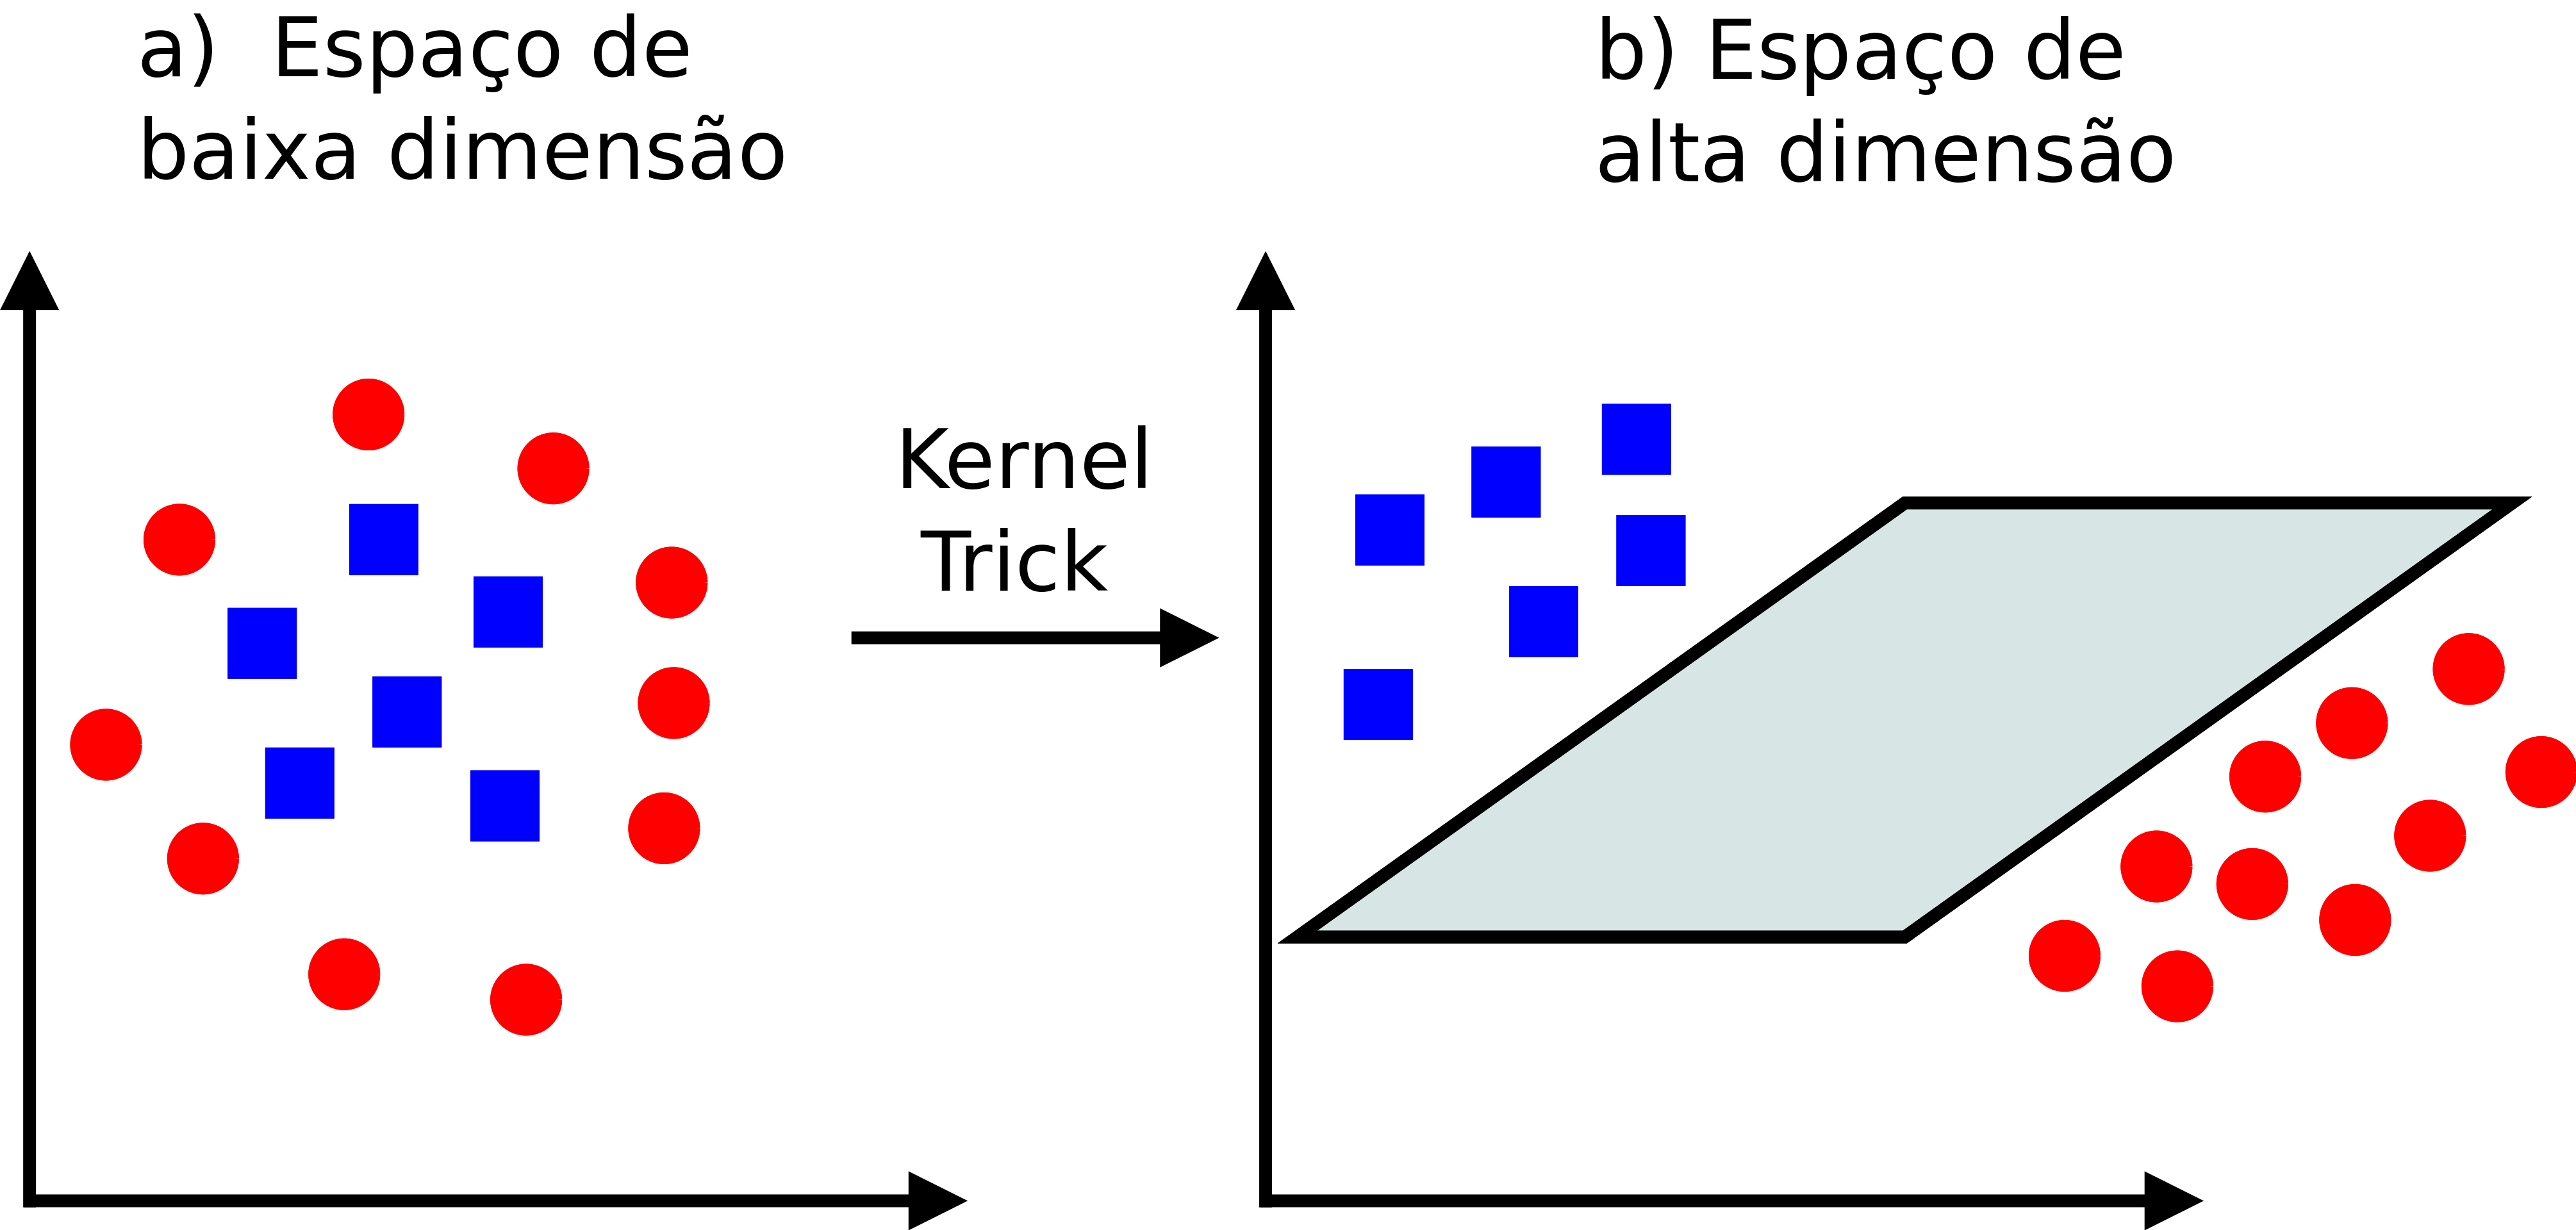
\includegraphics[width=11cm,height=5cm]{./secoes/conceitosFundamentais/pics/img/kernelTrick.png}
  \label{FIGURA_SVM_Caso_Nao_Separavel_KERNEL_TRICK}
  \source{Adaptado de \citeonline{MachineLearningwithR2013}.}
\end{figure}
Para compreender este mapeamento serão alteradas alguns detalhes das soluções já apresentadas para os casos anteriores. A equação \eqref{EQU_SVM_W_OTIMO} será reescrita como
\begin{align}
\sum\limits_{i=1}^{N_{S}} \alpha_{i}d_{i}\mathbf{\phi^{T}}(x_{i})\mathbf{\phi}(x) = 0
\end{align}
onde a função \(\mathbf{\phi^{T}}(x_{i})\mathbf{\phi}(x_{i})\) é um produto interno de valores que pode ser definido como
\begin{align}
k(x, x_{i}) = \mathbf{\phi^{T}}(x_{i})\mathbf{\phi}(x) \label{KERNEL_GENERICO}
\end{align}
onde a equação \eqref{KERNEL_GENERICO} é um Kernel, o qual é responsável por mapear os dados em alta dimensão \cite{Shawe2004}. Agora é possível reescrever o hiperplano ótimo como
\begin{align}
\sum\limits_{i=1}^{N_{S}} \alpha_{i}d_{i}k(\mathbf{x}, \mathbf{x_{i}}) = 0
\end{align}
com o uso da função de kernel \(k\) é desnecessário calcular o vetor de pesos ótimo \(\mathbf{w_{0}}\), este fato é conhecido por kernel trick. Por fim, com o uso do kernel trick é possível reescrever o problema de otimização dual como
\begin{align}
Q(\alpha) = \sum\limits_{i=1}^{N} \alpha_{i} - \frac{1}{2} \sum\limits_{i=1}^{N} \sum\limits_{j=1}^{N} \alpha_{i}\alpha_{j}d_{i}d_{j} k(\mathbf{x_{i}}, \mathbf{x_{j}})
\end{align}
com as restrições
\begin{align}
\sum\limits_{i=1}^{N} \alpha_{i}d_{i} &= 0 \\
0 < \alpha_{i} &\leq C	\qquad \textrm{ para } i = 1, 2, 3, \ldots, N
\end{align}
que é idêntico ao caso não separável acrescido da função de kernel. Alguns tipos de função Kernel conhecidas \cite{Haykin2007} são
\begin{align}
\textrm{Polinomial } &= ((x_{i}^{T} \cdot x_{j})+1)^{p}								\\
\textrm{Gaussiano }  &= \exp(\frac{-||x_{i}^{T} \cdot x_{j}||^{2}}{2\sigma^{2}})	\\
\textrm{Sigmóide }   &= \tanh(\beta_{0} (x_{i}^{T} \cdot x_{j})) +  \beta_{1} 		\\
\textrm{Linear }   &= (xy)
\end{align}


\section{Recomendação por regressão}\label{SEC_RECOMENDACAO_REGRESSAO}
Segundo \citeonline{HanKamber2011} a diferença entre classificar e efetuar uma regressão é que a última tem por objetivo predizer valores contínuos ao invés de discretos.

\subsection{Regressão com SVM}
O SVM para regressão tem um objetivo oposto ao classificador, enquanto o último tenta maximizar a margem (separando ao máximo os dados) o primeiro tem por objetivo aproximar os dados ao maximo dessa margem com uma dada tolerância para erros XXXXXXXX. Dado este objetivo será utilizado um procedimento de minimização de erro assãbsoluto para determinar o SVM para regressões, será utilizada a seguinte função de perda (a ser minimizada)
\begin{align}
L_{\epsilon} = 	\begin{cases}
						|d - y| - \epsilon  \qquad	\textrm{ para } |d - y| \geq \epsilon \\
						0					\qquad	\textrm{caso contrário}
				\end{cases}
\end{align}
considerando a restrição de robustez podemos escrever o problema de otimização como
\begin{align}
\nonumber \textrm{minimizar}\\
\frac{1}{2}||w||^{2} + C \sum\limits_{i=1}^{N} \xi_{i} + \xi_{i}^{'}\\
\nonumber \textrm{para as restrições}\\
y_{i} - (w \cdot x) - b \leq \epsilon + \xi_{i}\\
(w \cdot x) + b - y_{i}  \leq \epsilon + \xi_{i}^{'}\\
\xi_{i}^{'}, \xi_{i} \geq 0 \qquad \textrm{ para } i =1, 2, 3 \ldots N
\end{align}
utilizando as restrições é possível construir o Lagrangiano Primal
\begin{align}
J(w,\xi_{i}^{'}, \xi_{i}, \alpha, \alpha^{'}, \gamma, \gamma^{'}) = \frac{1}{2}||w||^{2} + C \sum\limits_{i=1}^{N} \xi_{i} + \xi_{i}^{'} - \sum\limits_{i=1}^{N} \gamma\xi_{i} + \gamma^{'}\xi_{i}^{'} \\
-\sum\limits_{i=1}^{N}\alpha_{i}((w \cdot x) + b - y_{i}+ \epsilon + \xi_{i}) \\
- \sum\limits_{i=1}^{N}\alpha_{i}^{'}(y_{i} - (w \cdot x) - b +\epsilon + \xi_{i}) \label{EQU_SVM_REGRESSAO_LAGRANGIANO_PRIMAL}
\end{align}
agora é necessário minimizar o Lagrangiano \eqref{EQU_SVM_REGRESSAO_LAGRANGIANO_PRIMAL} para isso devemos tomar as derivadas parciais em relação a \(w\), \(b\), \(\xi_{i}\) e \(\xi_{i}^{'}\) igualando-os a zero obtendo
\begin{align}
\hat{w} = \sum\limits_{i=1}^{N} (\alpha - \alpha^{'})x \label{EQU_SVM_REGRESSAO_PESO_W} \\
\sum\limits_{i=1}^{N} (\alpha - \alpha^{'}) = 0\\
\alpha + \gamma = C\\
\alpha^{'} + \gamma^{'} = C
\end{align}
o parâmetro desejado \(\hat{w}\) foi obtido pela equação \eqref{EQU_SVM_REGRESSAO_PESO_W} em função dos multplicadores de Lagrange \(\alpha^{'}, \alpha\). O valor de \(\hat{b}\) pode ser obtido pelas condições de KKT que aplicadas nas restrições do problema ficam como
\begin{align}
\alpha(\epsilon + \xi_{i} + d_{i} + y_{i}) = 0 \label{EQU_SVM_REGRESSAO_KKT1}\\
\alpha^{'}(\epsilon + \xi_{i}^{'} + d_{i} + y_{i}) = 0 \label{EQU_SVM_REGRESSAO_KKT2}\\
(C-\alpha)\xi_{i} = 0 \label{EQU_SVM_REGRESSAO_KKT3}\\
(C-\alpha^{'})\xi_{i}^{'} = 0 \label{EQU_SVM_REGRESSAO_KKT4}
\end{align}
analisando as equações \eqref{EQU_SVM_REGRESSAO_KKT1}, \eqref{EQU_SVM_REGRESSAO_KKT2}, \eqref{EQU_SVM_REGRESSAO_KKT3} e \eqref{EQU_SVM_REGRESSAO_KKT4} pode-se concluir que instâncias onde \(C=\alpha\) ou \(C=\alpha^{'}\) residem fora das variáveis de folga \(\xi_{i}\) e \(\xi_{i}^{'}\). Multiplicando \eqref{EQU_SVM_REGRESSAO_KKT1} por \(\alpha\) e \eqref{EQU_SVM_REGRESSAO_KKT2} por \(\alpha^{'}\) pode-se escrever
\begin{align}
\alpha\alpha^{'}(2\epsilon + \xi_{i} + \xi_{i}^{'})=0
\end{align}
sempre que \(\epsilon > 0, \xi_{i} > 0 e \xi_{i}^{'} > 0\) implica que \(\alpha\alpha^{'} = 0\). Pelas equações \eqref{EQU_SVM_REGRESSAO_KKT3} e \eqref{EQU_SVM_REGRESSAO_KKT4} pode-se escrever
\begin{align}
\xi_{i}  = 0		\qquad \textrm{ para } 0 < \alpha < C		\label{EQU_SVM_REGRESSAO_CONDICAO1}\\
\xi_{i}^{'} = 0		\qquad \textrm{ para }  0 < \alpha^{i} < C	\label{EQU_SVM_REGRESSAO_CONDICAO2}
\end{align}
as equações \eqref{EQU_SVM_REGRESSAO_CONDICAO1} e \eqref{EQU_SVM_REGRESSAO_CONDICAO2} implicam que  
\begin{align}
\epsilon  + d_{i} + y_{i} 	\qquad \textrm{ para } 0 < \alpha < C				\label{EQU_SVM_REGRESSAO_CONDICAO3}\\
\epsilon  + d_{i} + y_{i}	\qquad \textrm{ para }  0 < \alpha^{i} < C				\label{EQU_SVM_REGRESSAO_CONDICAO4}
\end{align}
com as equações \eqref{EQU_SVM_REGRESSAO_CONDICAO3} e \eqref{EQU_SVM_REGRESSAO_CONDICAO4} é possível calcular o \(\hat{b}\) sabendo que o estimador ótimo é dado por
\begin{align}
y = \hat{w}^{T}x + b \\
\nonumber\textrm{substituindo pela instância i} \\
y = \hat{w}^{T}x_{i} + b \label{EQU_SVM_REGRESSAO_CONDICAO5}
\end{align}
substituindo a equação \eqref{EQU_SVM_REGRESSAO_CONDICAO5} nas equações \eqref{EQU_SVM_REGRESSAO_CONDICAO3} e \eqref{EQU_SVM_REGRESSAO_CONDICAO4} ten-se que
\begin{align}
\hat{b} = d_{i} -\hat{w}^{T}x -\epsilon	\qquad \textrm{ para } 0 < \alpha < C		\label{EQU_SVM_REGRESSAO_CONDICAO6}\\
\hat{b} = d_{i} -\hat{w}^{T}x +\epsilon	\qquad \textrm{ para }  0 < \alpha^{i} < C	\label{EQU_SVM_REGRESSAO_CONDICAO7}
\end{align}
Com o valor de \(\hat{w}\) obtido da equação \eqref{EQU_SVM_REGRESSAO_PESO_W} e dados \(\epsilon\) e \(d_{i}\) é possível computar \(\hat{b}\).

\subsection{MARS}
O algoritmo \emph{Multivariate Adaptive Regression Splines}(MARS) segundo \citeonline{StatisticalLearning2001} é uma generalização da regressão linear por função degrau. Para tal usa-se segmentos lineares de funções com a seguinte estrutura:
\begin{align}
(x-t)_{+} &= \begin{cases}
x-t, \mbox{se } x>t \\
0,   \mbox{cc}
\end{cases}
\\
(t-x)_{+} &= \begin{cases}
t-x, \mbox{se } x<t \\
0, cc
\end{cases} 
\end{align}
como na Figura \ref{FIGURA_MARS_FUNCAO_ESPELHO} onde são visualisadas as funções espelho \((x-0.5)_{+}\) e \((0.5-x)_{+}\) cada uma é linear em um segmento e possuí um nó no valor de \(x\). Os segmentos de funções lineares (\emph{basis functions}) seguem a estrutura:
\begin{align}
C &= \{(X_{j}-t)_{+}(t-X_{j})_{+}\} \\
\nonumber t &\in {x_{1j}, x_{2j}, \ldots x_{Nj}}\\
\nonumber j &= 1, 2, \ldots p.
\end{align}
A ideia é formar pares de funções espelhos para cada variável independente \(X_{j}\) com um nó para cada valor de \(x_{i,j}\) daquela variável.
\begin{figure}[H]
	\centering
 	  \caption{Funções espelho usadas pelo MARS}
		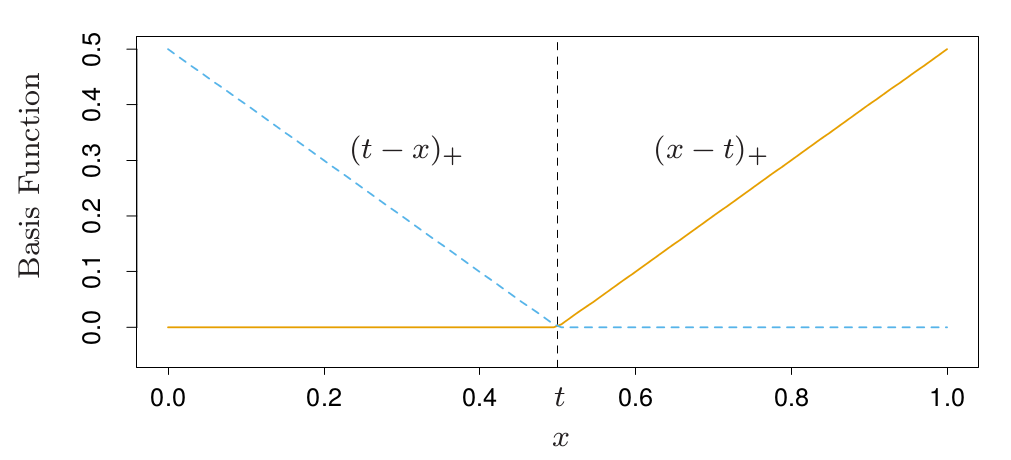
\includegraphics[width=11cm,height=6cm]{./secoes/conceitosFundamentais/pics/img/MARS_FUNCAO_ESPELHO.png}
	\label{FIGURA_MARS_FUNCAO_ESPELHO}
  \source{\citeonline{StatisticalLearning2001}}
\end{figure}
O modelo de regressão MARS tem o seguinte formato:
\begin{align}
f(X) = \beta_{0} + \sum\limits_{m=1}^{M}\beta_{m}h_{m}(X)
\end{align}
onde \(h_{m}(X)\) é uma função em \(C\) ou o produto de duas ou mais funções, os coeficientes \(\beta_{m}\) são estimados pela minimização da soma do resíduo quadrado

O algoritmo começa com uma função \(h_{0} = 1\), as funções do conjunto \(C\) são possíveis candidatas a serem adicionadas no conjunto de candidatos para \(h_{m}\) denominado \(M\) o seguinte produto:
\begin{align}
\beta_{M+1}h_{l}(X) \cdot (X_{j}-t)_{+} + \beta_{M+2}h_{l}(X) \cdot (t-X_{j})_{+} \\
\nonumber h_{l} \in M
\end{align}
tal que produza o menor incremento no erro de treinamento, os coeficientes \(\beta\) são estimados por minimos quadrados, esse processo continua até que \(M\) contenha um número de termos estabelecido. O modelo resultante tende a causar \emph{overfitting} nos dados, o algoritmo MARS soluciona este problema com uma estratégia de poda que inicia ao término  do processo anterior. A poda remove termo a termo tal que diminua ao máximo o erro residual quadrado para cada número de termos no modelo \(\lambda\). Este valor pode ser estimado por meio de minimização do GCV:
\begin{align}
GCV(\lambda) = \frac{\sum\limits_{i=1}^{N}(y_{i} - f_{\lambda}(x_{i}))^{2}}{(1-\frac{M(\lambda)}{N})^{2}}
\end{align}
onde \(f_{\lambda}\) é o valor estimado para \(\lambda\) termos, \(y_{i}\) é o valor ideal, \(N\) é o número de modelos a serem validados, \(M(\lambda)\) é o número de termos utilizados no modelo. Nesse ponto o modelo está treinado e pronto para uso como regressor.

\subsection{Regressão Logística}
A regressão logística usa um modelo estatístico para prever o comportamento de uma variável em função de outras. Para tal é utilizada uma generalização de modelos da família exponencial denominada \emph{modelos generalizados lineares}:
\begin{align}
y = X \beta + e
\end{align}
onde \(e\) é um vetor de erros. Essa generalização assume que a variável dependente (\(y\)) pode ter qualquer distribuição da família exponencial, existe uma função \emph{link} que:
\begin{align}
g(\mu) = \eta = \mathbf{X}\beta
\end{align}
relaciona a média da distribuição de probabilidade (\(\mu\)) as variáveis independentes (\(\mathbf{X}\)) e \(\beta\) é um vetor de parâmetros que devem ser estimados.
A família exponencial segue a fórmula genérica:
\begin{align}
f(y, \theta, \phi) = \exp \left( \frac{( y(\theta) - b(\theta) )} {a(\phi)} + c(y, \phi)\right) \label{EQU_FAMILIA_EXPONENCIAL}
\end{align}
onde \(a, b \) e \( c\) são funções, \(\phi\) é uma constante, \(\theta\) são os parâmetros da distribuição. A equação \ref{EQU_FAMILIA_EXPONENCIAL} satisfaz as distribuições: Poison, Normal, Bernoulli, Binomial. No caso da regressão logística temos:
\begin{align}
f(y, p) &=  \binom{n}{y} p^{y}(1 - p)^{n - y} \\
		&= \exp \left[ y\log \left( \frac{p}{1 - p} \right) + n\log(1-p) + \log \binom{n}{y} \right] \label{EQU_FAMILIA_EXPONENCIAL_BINOMIAL}
\end{align}
tomando \(\theta = \log \left( \frac{p}{1 - p} \right)\) e \( p = \frac{\exp(\theta)}{1+\exp(\theta)} \) e substituindo na equação \eqref{EQU_FAMILIA_EXPONENCIAL_BINOMIAL} obtemos:
\begin{align}
f(y, p) &= \exp \left[ y\theta + n\log(\frac{1}{1+\exp(\theta)}) + \log \binom{n}{y} \right]	\label{EQU_FAMILIA_EXPONENCIAL_BINOMIAL_PARAMETROS_SUBSTITUIDOS}
\end{align}
A equação \eqref{EQU_FAMILIA_EXPONENCIAL_BINOMIAL_PARAMETROS_SUBSTITUIDOS} pertence a família exponencial (ver equação \eqref{EQU_FAMILIA_EXPONENCIAL}) tomando \(\theta = \log \left( \frac{p}{1 - p} \right)\), \(b(\theta) = n\log[1+\exp(\theta)]\), \(c(y, \phi) = \log \binom{n}{y}\) e \(a(\phi) = 1\).
A estimação de parâmetros do modelo é feito por meio da maximização da máxima verossimilhança, uma possível abordagem é usar o algoritmo de \emph{Newton-Raphson}
para tal.

Um \emph{modelo generalizado linear} tem três componentes: i) a distribuição da variável dependente(neste caso binomial); ii) o preditor linear \(\alpha + \beta X = \frac{p}{1 - p} \); e iii) a função \emph{link} que relaciona a média da distribuição com o preditor linear, no nosso caso é \(g(\mu) = \log(\frac{p}{1-p})\)
